% =====================================================================================
% Complete Research and Implementation Report
%
% Build:  pdflatex report.tex   (three passes, for the ToC, LoF and LoT)
% Figures are pulled from ../docs/images and ../experiments/results via \graphicspath,
% so the report always shows the same files the manuscript embeds.
%
% Anything in report/generated/ is written by tools/build_report_data.py directly from
% the repository. Do not edit those files by hand; they exist so that counts, file lists
% and versions in this report cannot drift from the artefacts they describe.
% =====================================================================================
\documentclass[11pt,a4paper,oneside]{report}

\usepackage[T1]{fontenc}
\usepackage[utf8]{inputenc}
\usepackage{lmodern}
\usepackage[a4paper,left=1.3in,right=1in,top=1.1in,bottom=1.1in]{geometry}
\usepackage{graphicx}
\usepackage{booktabs}
\usepackage{longtable}
\usepackage{amsmath,amssymb}
\usepackage{listings}
\usepackage{xcolor}
\usepackage{fancyhdr}
\usepackage{titlesec}
\usepackage{caption}
\usepackage{enumitem}
\usepackage[hidelinks]{hyperref}
\usepackage{microtype}
% Lets an underscore appear literally in \code{...} and in prose, instead of needing \_
% at every call site. The [strings] option keeps it safe inside \label and \ref.
\usepackage[strings]{underscore}

\graphicspath{{../docs/images/}{../experiments/results/}{generated/}}
\newcommand{\repohead}{5fbe123}
\newcommand{\repohashfull}{5fbe1235a6633c6cef58a8e5e4c2a2c77c6b2ce4}
\newcommand{\srcfiles}{64}
\newcommand{\srccode}{7293}


\hypersetup{
  pdftitle={Unverified Assumptions in Embedded Safety Firmware: Research and Implementation Report},
  pdfauthor={MD Humayun},
  pdfsubject={M.Tech research and implementation report, SVNIT Surat},
}

% ---- page style
\pagestyle{fancy}
\fancyhf{}
\fancyhead[L]{\small\nouppercase{\leftmark}}
\fancyhead[R]{\small\thepage}
\renewcommand{\headrulewidth}{0.4pt}
\fancypagestyle{plain}{\fancyhf{}\fancyhead[R]{\small\thepage}%
  \renewcommand{\headrulewidth}{0pt}}

% ---- headings
\titleformat{\chapter}[display]
  {\normalfont\Large\bfseries}{\chaptertitlename\ \thechapter}{10pt}{\LARGE}
\titlespacing*{\chapter}{0pt}{-20pt}{24pt}

% ---- captions
\captionsetup{font=small,labelfont=bf,width=0.92\textwidth}

% ---- code listings
\definecolor{lsbg}{gray}{0.97}
\definecolor{lskw}{RGB}{20,70,140}
\definecolor{lscm}{RGB}{90,110,90}
\definecolor{lsst}{RGB}{150,60,40}
\lstset{
  basicstyle=\ttfamily\scriptsize,
  keywordstyle=\color{lskw}\bfseries,
  commentstyle=\color{lscm}\itshape,
  stringstyle=\color{lsst},
  backgroundcolor=\color{lsbg},
  frame=single,
  rulecolor=\color{gray!40},
  numbers=left,
  numberstyle=\tiny\color{gray},
  numbersep=7pt,
  breaklines=true,
  breakatwhitespace=false,
  columns=fullflexible,
  keepspaces=true,
  showstringspaces=false,
  tabsize=2,
  captionpos=b,
  xleftmargin=16pt,
  framexleftmargin=16pt,
}
\lstdefinestyle{cpp}{language=C++,morekeywords={constexpr,static_assert,uint8_t,uint32_t,
  size_t,nullptr,override,TaskHandle_t,QueueHandle_t,SemaphoreHandle_t,BaseType_t,TickType_t}}
\lstdefinestyle{py}{language=Python}
\lstdefinestyle{tla}{morekeywords={MODULE,EXTENDS,CONSTANT,CONSTANTS,VARIABLES,ASSUME,
  THEOREM,Init,Next,Spec,UNCHANGED,ENABLED,TRUE,FALSE,IF,THEN,ELSE,LET,IN},
  morecomment=[l]{\\*},sensitive=true}
\lstdefinestyle{sh}{language=bash}

\newcommand{\code}[1]{\texttt{\small #1}}

\begin{document}

% =====================================================================================
% PRELIMINARY PAGES
% =====================================================================================
\pagenumbering{roman}
\begin{titlepage}
\centering
\thispagestyle{empty}

{\large SARDAR VALLABHBHAI NATIONAL INSTITUTE OF TECHNOLOGY, SURAT}\\[2pt]
{\normalsize Department of Computer Science and Engineering}\\[36pt]

\rule{\textwidth}{0.8pt}\\[14pt]
{\LARGE\bfseries Unverified Assumptions in Embedded\\[4pt] Safety Firmware}\\[10pt]
{\large Configuration, Specification and Response-Time Defects\\ in an MQTT Alarm System}\\[12pt]
\rule{\textwidth}{0.8pt}\\[26pt]

{\normalsize\itshape Research and Implementation Report}\\[30pt]

\begin{tabular}{@{}r@{\hskip 1.2em}l@{}}
\textbf{Submitted by}   & MD Humayun \\
\textbf{Admission No.}  & P25IS016 \\
\textbf{Programme}      & M.Tech, Computer Science and Engineering \\
                        & Specialisation: Information Security and Privacy \\
\textbf{Semester}       & M.Tech II, Semester III \\
\textbf{Academic year}  & 2026--2027 \\[14pt]
\textbf{Supervisor}     & Dr.\ M.\ A.\ Zaveri \\
                        & Department of Computer Science and Engineering \\
                        & SVNIT Surat \\
\end{tabular}

\vfill

\begin{tabular}{@{}r@{\hskip 1.2em}l@{}}
\textbf{Repository}  & \texttt{github.com/mdhumayun7/Smart-Home-Automation} \\
\textbf{Commit}      & \texttt{\repohashfull} \\
\textbf{Report date} & 7 November 2026 \\
\end{tabular}

\vspace{18pt}
{\small\itshape This report accompanies a research manuscript prepared for journal
submission. The manuscript and this report are separate documents with different purposes;
Section~\ref{sec:intro-scope} explains the relationship.}
\end{titlepage}

\chapter*{Declaration}
\addcontentsline{toc}{chapter}{Declaration}
\markboth{Declaration}{}

\noindent I declare that the work presented in this report is my own, carried out under the
supervision of Dr.\ M.\ A.\ Zaveri in the Department of Computer Science and Engineering at
Sardar Vallabhbhai National Institute of Technology, Surat.

\vspace{8pt}
\noindent Specifically:

\begin{itemize}[leftmargin=1.4em,itemsep=3pt]
  \item The firmware, formal specifications, experimental harnesses, analysis scripts and
        figure generators described here were written by me and are committed to the
        repository named on the title page.
  \item Every experimental result reported is produced by those committed scripts and
        regenerates from the seeds recorded with it. Where a figure or table reports a number,
        that number is recomputed from the raw per-trial records by
        \code{experiments/validate\_figures.py}.
  \item Work by others is cited where it is used. The only numerical results in this report
        that are not my own are the cycle-loss measurements of Behnke et al., which are
        attributed to them wherever they appear.
  \item \textbf{No physical hardware measurement is reported.} Chapter~\ref{ch:limitations}
        states what has and has not been measured, and the hardware conditions described in
        Appendix~\ref{app:hardware} have not been executed.
  \item An AI assistant was used for drafting, documentation, code review and literature
        discovery. All research claims, experimental designs, results and conclusions are my
        own; I reviewed and verified the content and take full responsibility for it. The
        accompanying manuscript carries the corresponding declaration in the form the
        publisher requires.
\end{itemize}

\vspace{36pt}
\noindent\begin{tabular}{@{}p{0.45\textwidth}p{0.45\textwidth}@{}}
\rule{0.9\linewidth}{0.4pt} & \rule{0.9\linewidth}{0.4pt} \\
MD Humayun \quad (P25IS016) & Date \\
\end{tabular}

\vspace{20pt}
\noindent\textit{\small This page is a draft prepared for the author's signature. It is
unsigned and carries no approval.}

\chapter*{Certificate}
\addcontentsline{toc}{chapter}{Certificate}
\markboth{Certificate}{}

\vspace{10pt}
\noindent This is to certify that the work contained in this report, entitled
\emph{Unverified Assumptions in Embedded Safety Firmware: Configuration, Specification and
Response-Time Defects in an MQTT Alarm System}, submitted by \textbf{MD Humayun}
(Admission No.\ P25IS016) to the Department of Computer Science and Engineering, Sardar
Vallabhbhai National Institute of Technology, Surat, was carried out under my supervision.

\vspace{50pt}
\noindent\begin{tabular}{@{}p{0.45\textwidth}p{0.45\textwidth}@{}}
\rule{0.9\linewidth}{0.4pt} & \rule{0.9\linewidth}{0.4pt} \\
Dr.\ M.\ A.\ Zaveri & Head of Department \\
Supervisor & Computer Science and Engineering \\
Computer Science and Engineering & SVNIT Surat \\
SVNIT Surat & \\
\end{tabular}

\vspace{40pt}
\begin{center}
\fbox{\begin{minipage}{0.86\textwidth}
\small\textbf{Template only.} This page is an unsigned template reproducing the form the
department normally requires. No signature, endorsement, approval or examiner comment has
been obtained or reproduced, and none should be inferred from its presence here. It is
included so the report can be completed through the department's own process.
\end{minipage}}
\end{center}

\chapter*{Acknowledgement}
\addcontentsline{toc}{chapter}{Acknowledgement}
\markboth{Acknowledgement}{}

\noindent I am grateful to my supervisor, Dr.\ M.\ A.\ Zaveri, for guidance throughout this
work, and in particular for the insistence on separating what has been measured from what has
been argued. Several of the corrections recorded in this report---the vacuous invariant in
Chapter~\ref{ch:formal} above all---came from taking that distinction seriously rather than
from any new technique.

\vspace{6pt}
\noindent I thank the Department of Computer Science and Engineering at SVNIT Surat for the
facilities and the time that made this work possible.

\vspace{6pt}
\noindent The work builds directly on the measurements of Behnke et al., whose study of
real-time degradation on the ESP32 under network load defined the question this project set
out to answer. Their honesty about the limits of their own mitigations is what made the gap
visible.

\vspace{18pt}
\noindent\begin{tabular}{@{}l@{}}
MD Humayun \\
November 2026 \\
\end{tabular}

\vspace{20pt}
\noindent\textit{\small Draft. Names of anyone else who should be thanked are to be added by
the author before submission.}

\chapter*{Abstract}
\addcontentsline{toc}{chapter}{Abstract}
\markboth{Abstract}{}

\noindent Domestic intrusion alarms are now built almost entirely on single-chip Wi-Fi
systems-on-chip. On the ESP32, the radio driver, the TCP/IP stack, the MQTT client and the
alarm application share one die, one scheduler and one interrupt controller. Two pieces of
standard engineering advice are used to contain the resulting risk: pin the safety task to its
own core, and gate risky features behind build-time configuration. Both are assertions about
the system, and in practice neither is checked.

\vspace{6pt}
\noindent This work treats an ESP32 intrusion alarm as a case study and sets out to falsify
both assertions rather than to demonstrate them. Three defects were found, each residing in a
different kind of assumption, and each exposed by a method that costs considerably less than
the system it examines. A compile-time guard accepted the combination of TLS and a broker login
as evidence of a publisher's authority; under a single leaked credential the alarm fired in
only 16.7\% of 300 trials, against 100\% for the control. A response-time decomposition
exposed an unbounded command drain in the safety loop that 9,600 adversarial trials, 3,000,000
fuzzing iterations and exhaustive model checking had all passed over. The project's own
temporal-logic invariant forbidding unauthenticated remote disarm proved to be vacuous in the
specification that had been shipped and checked in continuous integration.

\vspace{6pt}
\noindent A twelve-configuration ablation over 3,600 trials shows that availability, integrity
and the safety function fail independently of one another: a token-bucket rate limiter costs
41\% of legitimate operator commands while contributing nothing to integrity. Broker access
control and application-layer message authentication were found to fail under different
compromises, a result reproduced against a live Mosquitto broker across eight scenarios. An
adversary in possession of a compromised controller host---holding both a credential the access
control list must permit and the command key---defeats the layered configuration and locks the
legitimate owner out of all 1,250 attempted commands.

\vspace{6pt}
\noindent An attempt to generalise the configuration finding across 135 commit-pinned
open-source embedded MQTT projects returned no hits for the guard pattern. That negative result
is reported as such, and no claim is made about the prevalence of the pattern in the wider
ecosystem.

\vspace{6pt}
\noindent The results establish \emph{logical} isolation only. Physical timing invariance is a
property of the silicon and of a closed-source radio driver; it has not been measured, no
latency figure is reported, and the hardware protocol that would settle the question is
documented rather than executed.

\vspace{10pt}
\noindent\textbf{Keywords:} embedded systems security; MQTT; configuration defects;
specification mutation; response-time analysis; formal verification; ESP32


\cleardoublepage
\phantomsection
\addcontentsline{toc}{chapter}{Table of Contents}
\tableofcontents

\cleardoublepage
\phantomsection
\addcontentsline{toc}{chapter}{List of Figures}
\listoffigures

\cleardoublepage
\phantomsection
\addcontentsline{toc}{chapter}{List of Tables}
\listoftables

\chapter*{List of Abbreviations}
\addcontentsline{toc}{chapter}{List of Abbreviations}
\markboth{List of Abbreviations}{}

\begin{longtable}{@{}p{0.17\textwidth}p{0.78\textwidth}@{}}
\toprule
\textbf{Abbreviation} & \textbf{Expansion} \\
\midrule
\endhead
ACL      & Access Control List \\
ASan     & AddressSanitizer \\
APC      & Article Publishing Charge \\
CI       & Continuous Integration \\
CID      & Character Identifier (font encoding) \\
CRediT   & Contributor Roles Taxonomy \\
DUT      & Device Under Test \\
FSM      & Finite State Machine \\
GPIO     & General-Purpose Input/Output \\
HMAC     & Hash-based Message Authentication Code \\
I2C      & Inter-Integrated Circuit \\
IoT      & Internet of Things \\
ISR      & Interrupt Service Routine \\
JCR      & Journal Citation Reports \\
JSA      & Journal of Systems Architecture \\
LoC      & Lines of Code \\
MAC      & (a) Message Authentication Code; (b) Medium Access Control. Disambiguated at each use \\
MQTT     & Message Queuing Telemetry Transport \\
NVS      & Non-Volatile Storage (ESP32 key--value flash store) \\
OLED     & Organic Light-Emitting Diode \\
PIR      & Passive Infrared (motion sensor) \\
PUBACK   & MQTT publish acknowledgement \\
QoS      & Quality of Service (MQTT delivery class) \\
RF       & Radio Frequency \\
RTOS     & Real-Time Operating System \\
SCIE     & Science Citation Index Expanded \\
SHA      & Secure Hash Algorithm \\
SJR      & SCImago Journal Rank \\
SNIP     & Source Normalized Impact per Paper \\
SoC      & System-on-Chip \\
SVG      & Scalable Vector Graphics \\
TLA+     & Temporal Logic of Actions (specification language) \\
TLC      & The TLA+ model checker \\
TLS      & Transport Layer Security \\
UBSan    & UndefinedBehaviorSanitizer \\
WCET     & Worst-Case Execution Time \\
\bottomrule
\end{longtable}


% =====================================================================================
% CHAPTERS
% =====================================================================================
\cleardoublepage
\pagenumbering{arabic}

\chapter{Introduction}\label{ch:intro}

\section{Research background}

A domestic intrusion alarm has one obligation. When a sensor detects an intrusion, a siren must
sound within a bounded time. Everything else the device does — reporting state to a phone,
accepting remote commands, logging events — is secondary, and none of it excuses a failure to
make a noise.

The hardware on which these devices are now built makes that obligation harder to meet than it
first appears. A decade ago an alarm panel was a microcontroller with a dedicated radio module
or a wired connection. Today the entire device is typically one inexpensive
system-on-chip. On the Espressif ESP32, which is the platform studied here, a single die carries
two processor cores, the 802.11 radio and its closed-source driver, the TCP/IP stack, the TLS
implementation, the MQTT client and the alarm application itself. They share the scheduler, the
memory bus and the interrupt controller.

This matters because it creates a path from the outside world to the safety function that does
not exist in a system with separated hardware. An attacker who cannot reach the alarm's logic
directly may still be able to load the shared resources enough to delay it. The attacker needs
no credentials, no access to the building and no knowledge of the application: radio-layer
frames are processed beneath the IP stack whether or not any socket is listening.

\subsection{Embedded safety firmware}

The term \emph{safety firmware} is used in this report for the portion of an embedded program
whose correct and timely execution is the reason the device exists. In an alarm this is the
sensor-conditioning code, the state machine that decides whether the system is armed, and the
output driver that energises the siren.

Two properties distinguish safety firmware from the rest of a program. First, its obligation is
a \emph{bound}, not an average: an alarm that usually sounds in 150\,ms and occasionally takes
four seconds has failed, even though its mean is excellent. Second, it must continue to work
when the rest of the system does not. A loss of network connectivity, a broker outage or a
saturated radio must not prevent the siren from sounding, because the circumstances under which
an alarm is most needed are precisely the circumstances in which the network is least reliable.

Developers of such firmware on dual-core microcontrollers are given two standard pieces of
advice, which this work takes as its subject:

\begin{enumerate}[leftmargin=1.6em,itemsep=4pt]
  \item \textbf{Pin the safety task to its own core}, and place everything network-facing on
        the other, so that network work cannot delay safety work.
  \item \textbf{Gate risky features behind build-time configuration}, so that a dangerous
        capability is compiled out unless the build deliberately asks for it.
\end{enumerate}

Both are reasonable. Both are also \emph{assertions} about the system rather than
demonstrated properties — the first asserts something about timing, the second something about
security — and in ordinary practice neither is tested. That gap is the subject of this work.

\subsection{MQTT-based communication}

MQTT is the dominant application protocol for this class of device. It is a publish--subscribe
protocol in which clients connect to a central broker, publish messages to topics, and
subscribe to topics they wish to receive. Its appeal for constrained devices is real: the
protocol is small, the client libraries are small, and a device behind a domestic router needs
no inbound connectivity, because it establishes an outbound connection to the broker and
receives commands over it.

The architectural consequence is less often discussed, and it is central to
Chapter~\ref{ch:security}. The broker is not a transparent pipe. It terminates each client's
transport connection and \emph{re-originates} every message it forwards. A device receiving a
command therefore receives it from the broker, over the device's own TLS connection to the
broker, with no cryptographic evidence of which client originally published it. Transport
security protects each hop; it conveys nothing about provenance across the relay. MQTT 3.1.1
compounds this by providing no return code meaning ``refused by policy'': a broker that
discards a publication for violating an access control list still acknowledges it, so the
publisher cannot distinguish success from silent refusal.

\subsection{Security challenges in connected IoT systems}

Three difficulties recur in this device class and all three appear in the results reported
here.

\textbf{Credentials are shared with the device.} A device that authenticates to a broker must
hold a credential, and that credential lives in flash on a physically accessible object. The
same is true of any application-layer key. If both are in the same image, an adversary who
extracts one extracts the other — a point that turns out to determine which of two defences
survives which compromise (Section~\ref{sec:sec-flashdump}).

\textbf{The controlling host is part of the trust boundary.} A phone or home-automation server
that legitimately issues commands must hold whatever authority is needed to issue them. Its
compromise therefore yields that authority, and no amount of care inside the device can prevent
it. Chapter~\ref{ch:security} reports this as the configuration that defeats the strongest
design evaluated here.

\textbf{Availability and integrity are separate properties and trade against each other.} A
rate limiter improves resistance to flooding and degrades legitimate availability. A static
shared token preserves availability and provides no replay resistance. The ablation in
Section~\ref{sec:res-ablation} measures this independence rather than assuming it.

\subsection{Why reliable intrusion alarms matter}

The case for taking this seriously does not rest on sophistication. These devices are cheap,
numerous, installed by non-specialists and rarely updated. A homeowner who installs one has
made a decision about physical security on the strength of an implicit promise about timing and
authority. An alarm that can be silenced from outside the building by an adversary with a
leaked credential, or delayed past the point of usefulness by radio-layer noise, has broken
that promise in a way that is invisible until it matters.

The installed base is also large enough that a defect in the standard engineering advice is
worth more attention than a defect in any single product.

\section{Motivation}

The direct motivation is a measurement by Behnke et al.\ \cite{behnke2020}, who instrumented a
periodic critical task on an ESP32 and subjected the device to IP packet load. They found
measurable degradation: the task lost between 2.15\% and 3.8\% of its cycles for packets
addressed to a port it was listening on, and between 3.17\% and 6.67\% for an unused port, with
latency rising as the microcontroller saturated. Their conclusion was that command-and-control
over IP is unsuitable for hard real-time work on devices of this kind.

That result settles one question and opens three, and those three define this project.

\begin{enumerate}[leftmargin=1.6em,itemsep=4pt]
  \item \textbf{It measures the phenomenon but does not evaluate a mitigation.} The follow-up
        work from the same group proposes two \cite{behnke2022,behnke2023}, but neither is
        available to a developer shipping a stock ESP32: the first was evaluated against a
        simulated network interface and never built, and the second was prototyped on a Xilinx
        Zynq-7000, a considerably larger platform. Notably, \cite{behnke2023} uses the ESP32's
        second core to separate the observed process from the test harness rather than as a
        mitigation, so \emph{core pinning is nowhere evaluated as a defence}.
  \item \textbf{All the load in that line of work is applied at the IP layer.} The attack that
        actually threatens a wireless alarm is deauthentication — 802.11 management frames
        handled in the MAC layer and the radio driver, beneath the IP stack, which the device
        must process whether or not a socket is listening. Whether this interference path
        behaves like IP load is unknown.
  \item \textbf{No treatment of the isolation argument is formal, and none models an
        adversary} rather than volumetric stress.
\end{enumerate}

A second motivation emerged during the work itself and ultimately shaped the paper more than
the first. In the course of trying to verify the two standard assertions, three defects were
found \emph{in this project's own artefacts} — not in third-party code. Each had survived the
techniques one would normally rely on. That experience, rather than any single finding, is what
the research reports.

\section{Research objectives}

\begin{enumerate}[leftmargin=2.2em,itemsep=4pt,label=\textbf{O\arabic*.}]
  \item Determine whether core pinning combined with bounded queue discipline is adequate as an
        isolation mitigation on a single-chip Wi-Fi SoC, and establish precisely which part of
        that question can be settled without physical measurement.
  \item Establish, formally, whether an adversary with remote command-interface access can
        affect the safety function's control or data flow.
  \item Determine experimentally which command-path defence preserves the safety function,
        operator availability and replay resistance, treating the three as separate properties
        rather than as one.
  \item Determine where broker-side authorisation and application-layer authentication fail,
        and whether either dominates the other under credential compromise.
  \item Derive a response-time bound for the safety loop and identify which interference terms
        can be settled analytically and which require hardware.
  \item Establish whether the configuration defect found in this system generalises to
        comparable open-source projects.
  \item Specify a measurement protocol capable of falsifying the timing claim that remains
        unresolved, and publish it whether or not it can be executed.
\end{enumerate}

\section{Scope of the work}\label{sec:intro-scope}

\subsection*{What is inside the scope}

One artefact is studied: an ESP32-WROOM-32 intrusion alarm, firmware v2.2.0, whose complete
source is in the repository. The evaluation covers its command path, its safety state machine,
its queue discipline, its broker authorisation and its application-layer authentication. The
evidence is of five kinds, kept separate throughout: formal verification, host simulation,
testbed measurement against a live broker, analysis, and a static corpus study.

\subsection*{What is outside the scope, and why}

\textbf{Physical timing measurement.} No latency figure is reported anywhere in this report or
in the accompanying manuscript. The simulation harness advances a logical clock, so it provides
no information about timing whatever. The hardware protocol that would settle the question is
specified in Appendix~\ref{app:hardware} and has not been run.

\textbf{Attack tooling.} The repository publishes no procedure or tool for generating
radio-layer attacks. This is deliberate, and it limits what can be reported about the one
condition that would need such tooling.

\textbf{Generality.} One chip, one application, two framework versions, no deployment. The
corpus study in Section~\ref{sec:res-corpus} was the attempt to generalise and it returned
nothing; that outcome is reported as a null result and no prevalence claim is made from it.

\subsection*{Relationship to the accompanying manuscript}

Two documents exist and they serve different purposes. The manuscript is prepared for journal
submission: it is concise, confined to what is defensible before reviewers, and formatted to
the target journal's requirements. This report documents the whole project — including the
development environment, the implementation at module level, the experimental apparatus, and
the defects found in the project's own measurement infrastructure along the way, which a
journal paper has no room for. Where the two overlap, the numbers are identical, because both
draw on the same committed records.

\section{Main contributions}

Eight contributions were claimed in an early draft. They were reduced to five after each was
classified against the literature, because the evidence does not support eight. The reduction
is recorded in \code{docs/CONTRIBUTIONS.md}.

The central claim is this:

\begin{quote}
A security property asserted in build configuration, and a timing property asserted in design,
are both unverified claims. Each can be falsified by a method that costs far less than the
system it checks.
\end{quote}

\begin{enumerate}[leftmargin=2.2em,itemsep=5pt,label=\textbf{C\arabic*.}]
  \item \textbf{A configuration defect that costs a safety property.} A compile-time guard
        accepted TLS plus a broker login as evidence of publisher authority. The inference is
        unsound because the broker re-originates messages. Under a single leaked credential the
        alarm fired in 16.7\% of 300 trials against 100\% for the control. The guard emitted no
        diagnostic and survived review. (Chapter~\ref{ch:security})
  \item \textbf{A response-time decomposition that exposed an unbounded drain.} The
        decomposition removes three of four interference terms by construction and, in doing
        so, revealed that the safety loop had no static bound on its own execution time. The
        defect had passed 9,600 adversarial trials, 3,000,000 fuzzing iterations, exhaustive
        model checking and 129 host tests. (Chapter~\ref{ch:impl}, Section~\ref{sec:impl-drain})
  \item \textbf{A disclosed vacuous invariant, and a regression test for vacuity.} The property
        stating that unauthenticated remote disarm never takes effect was unfalsifiable in the
        specification that was shipped and checked in CI, because it assumed the refusal rather
        than deriving it. The model-checking runner now \emph{requires} a deliberately
        defective configuration to fail. (Chapter~\ref{ch:formal})
  \item \textbf{A measurement of defence independence.} A twelve-configuration ablation over
        3,600 trials shows availability, integrity and the safety function failing
        independently, and shows broker authorisation and message authentication failing under
        different compromises — reproduced against a live broker.
        (Chapter~\ref{ch:results})
  \item \textbf{A published, falsifiable measurement protocol} for the timing question that
        remains open, together with an honest negative generalisation result from a
        commit-pinned corpus of 135 projects. (Appendix~\ref{app:hardware},
        Section~\ref{sec:res-corpus})
\end{enumerate}

No new mechanism, attack, protocol or formalism is claimed. Ablation, response-time analysis
and specification mutation are all established techniques. What the work reports is that
applying them to a system's \emph{assumptions}, rather than to its running behaviour, caught
three defects that testing the running behaviour did not.

\section{Organisation of this report}

Chapter~\ref{ch:lit} reviews the relevant literature and states the research gap.
Chapter~\ref{ch:req} gives the requirements, system assumptions and threat model.
Chapter~\ref{ch:arch} presents the architecture. Chapter~\ref{ch:tools} documents the
development environment with verified versions. Chapter~\ref{ch:impl} explains the
implementation module by module with code excerpts. Chapter~\ref{ch:method} documents the
experimental methodology and Chapter~\ref{ch:results} the results and their statistical
treatment. Chapter~\ref{ch:formal} covers formal verification. Chapter~\ref{ch:security}
discusses the security evaluation. Chapter~\ref{ch:figures} catalogues the figures.
Chapter~\ref{ch:limitations} states the limitations and threats to validity, and
Chapter~\ref{ch:conclusion} concludes. Eleven appendices carry the inventories, commands and
reproduction instructions.

\chapter{Literature Review and Research Gap}\label{ch:lit}

This chapter reviews the work this project builds on and states precisely where it stops. The
emphasis is on what each line of work establishes and what it leaves unresolved, because the
gap this project addresses is defined by the second of those more than the first.

All twenty-two references cited here are the ones carried by the accompanying manuscript. No
reference has been added for this report without its bibliographic details being checked
against the publisher, proceedings or preprint record.

\section{Real-time degradation from on-chip network activity}

The closest prior work, and the direct motivation for this project, is the study by Behnke et
al.\ \cite{behnke2020}. They instrumented a periodic critical task on an ESP32 and applied IP
packet load while measuring the task's lateness. The degradation they report is modest in
percentage terms but unambiguous: between 2.15\% and 3.8\% of cycles lost for traffic addressed
to a listened port, and between 3.17\% and 6.67\% for an unused port, with latency rising as
the microcontroller approached saturation. Their conclusion is that command-and-control over IP
is unsuitable for hard real-time work on this class of device.

Two aspects of that result deserve attention. The first is that interference is higher for the
\emph{unused} port than for the listened one, which is counter-intuitive until one notices that
it is consistent with cost being incurred below the application: the device pays for frame
reception and demultiplexing whether or not anything is waiting for the data. The second is
that the authors are explicit about the limits of their own mitigations, and it is that honesty
that makes the gap visible.

The same group proposed two mitigations in follow-up work. The first is a priority-aware
multiqueue network interface with per-flow interrupt moderation \cite{behnke2022}; the second is
driver-level early demultiplexing \cite{behnke2023}. Neither is available to a developer
shipping a stock ESP32 today. The multiqueue design was evaluated against a \emph{simulated}
network interface and was never built. The demultiplexing work was prototyped on a Xilinx
Zynq-7000 — a platform an order of magnitude larger than an ESP32 — with measurements taken on
a single core.

The detail that matters most for this project appears in \cite{behnke2023}: the ESP32's second
core is used there to separate the observed processes from the test harness, not as a
mitigation. \textbf{Core pinning is therefore nowhere evaluated as a defence} in this line of
work, despite being the mitigation that developers of these devices are actually told to use.

Fischer et al.\ \cite{fischer2020} examine industrial device architectures under
denial-of-service conditions and reach a compatible conclusion at a coarser granularity: device
architecture, rather than protocol choice, determines whether real-time behaviour survives
network stress. Their analysis is architectural rather than experimental at the task level, so
it frames the problem without constraining the answer for any specific chip.

\section{Timing isolation on larger platforms}

A substantial body of work addresses timing isolation where the hardware offers the means to
achieve it. Meszlényi et al.\ \cite{timingiso2025} develop timing isolation for
mixed-criticality communication, and Hoornaert et al.\ \cite{mcti2024} present task-based
isolation for mixed-criticality workloads. Burns and Davis's review \cite{mcreview2026}, now in
its fourteenth edition, surveys the field as a whole.

The common prerequisite in this literature is hardware support: memory-bandwidth regulation,
cache partitioning, interrupt steering, or a hypervisor. None of these exists on an ESP32. The
platform offers core affinity and the scheduler's priority mechanism, and nothing else. The
mixed-criticality literature is therefore highly relevant as a statement of what adequate
isolation requires, and inapplicable as a source of techniques for this device class. That
mismatch — a well-developed theory whose preconditions the hardware does not satisfy — is part
of why the standard advice for the ESP32 remains unverified rather than merely weak.

\section{Radio-layer attacks on this device class}

The attack that threatens a wireless alarm is not IP flooding. It is deauthentication: 802.11
management frames handled in the MAC layer and the radio driver, below the IP stack, which the
device must process regardless of what any application is doing.

Kremser and Graffi \cite{deauther2026} evaluate the ESP32-S3 for Wi-Fi penetration testing and
demonstrate that the hardware is itself a capable attack platform, which establishes that the
capability required is cheap and widely available. Cayre et al.\ \cite{espwn2023} examine the
ESP32's own wireless stack offensively, finding vulnerabilities at the system-on-chip level.
Mudraje et al.\ \cite{esp32c3re2025} reverse-engineer the ESP32-C3's Wi-Fi drivers, work
undertaken precisely because the driver is closed source — a fact with direct consequences for
this project, since an unanalysable driver is why one interference term in
Chapter~\ref{ch:impl}'s response-time decomposition cannot be settled analytically.

Carbajal and Jodeiri Akbarfam \cite{carbajal2026} provide a software-defined testbed for
quantifying deauthentication resilience. Their work is methodologically the nearest to the
hardware protocol specified in Appendix~\ref{app:hardware}, and it reinforces a constraint
observed here: experiments of this kind require an isolated radio environment, which is an
institutional rather than a technical prerequisite.

What this literature establishes is that the radio-layer attack path is real, cheap to mount
and distinct from the IP path. What it does not do is measure the \emph{safety} consequence on
a device whose safety task is pinned to a separate core. That is the question this project set
out to answer and, as Chapter~\ref{ch:limitations} states plainly, could not answer by
measurement.

\section{Finding defects in embedded firmware}

Yun et al.\ \cite{fuzzsurvey2022} survey fuzzing for embedded systems and identify the
recurring obstacle: embedded firmware is difficult to execute outside its target hardware, so
fuzzing campaigns must either run on the device, at low throughput, or rehost the firmware,
with fidelity loss.

Two recent systems address rehosting directly. Bley et al.\ \cite{pemu2025} present
protocol-aware firmware rehosting for fuzzing embedded network stacks; Tharindu et al.\
\cite{sysfuss2026} combine system-level firmware fuzzing with selective symbolic execution.
Both are substantially more capable than the approach taken here, and the comparison is worth
stating honestly: the fuzzing in this project compiles the parser \emph{for the host} and
exercises it under sanitizers. That is appropriate for the question asked — whether the command
parser mishandles malformed input — and it is explicitly \emph{not} firmware rehosting. It
says nothing about faults depending on the Xtensa toolchain's code generation, on the real
memory map, or on the radio driver's own parsing. Chapter~\ref{ch:limitations} records this as a
limitation rather than leaving it implicit.

The more important point for this work, however, is one the fuzzing literature does not
address. All of these techniques test a \emph{running system}. None of them tests the
\emph{assumptions a system was built on}. A build condition that encodes an unsound security
inference will compile, run, and pass every dynamic test, because dynamic testing exercises the
build that was produced rather than questioning whether that build should have been permitted.
The unbounded drain reported in Section~\ref{sec:impl-drain} makes the same point from the
timing side: it survived 3,000,000 fuzzing iterations because every one of those iterations
exercised a path that terminated.

\section{Security and verification on the ESP32 application stack}

Azhar et al.\ \cite{mqtttls2026} analyse the performance and security of MQTT over TLS on
ESP32-based systems, establishing the cost of the transport protection this project assumes as
a baseline. Ieropoulos et al.\ \cite{ondevice2026} place intrusion detection on constrained
devices, which is a different architectural answer to a related problem.

On the MQTT protocol itself, Zeghida et al.\ \cite{zeghida2024} give an overview of security
issues, and Alsabbagh et al.\ \cite{pirates2024} demonstrate the attack class that this
project's configuration defect exposes: a rogue client with valid broker credentials raiding
industrial IoT systems. This citation matters for the integrity of the present work's claims.
\textbf{The attack class is published and the underlying principle is textbook}, so this project
claims no new vulnerability. Its contribution is narrower: that a \emph{compile-time guard} can
encode the unsound inference, emit no diagnostic, and thereby cost a safety property.

Two 2026 papers approach the same problem from the design side. Amirkhanova et al.\
\cite{amirkhanova2026} build an end-to-end encrypted data pipeline for industrial IoT, and Yu
et al.\ \cite{mqttl2026} propose MQTT-L, a lightweight end-to-end secure protocol using
renewable hash chains. Both confirm, from the direction of protocol design, the principle this
project confirms from the direction of failure analysis: end-to-end authentication is required
because the broker is a relay and transport security does not survive it.

On formal methods, Krichen's survey \cite{krichen2023} covers verification and validation for
the Internet of Things, including model checking, abstract interpretation and deductive
methods. Lamport \cite{lamport2002} is the reference for the specification language used here.
Neither addresses the failure mode reported in Chapter~\ref{ch:formal} — a specification that
assumes the property it claims to establish — which is a known hazard in the formal-methods
community but, as far as this review found, is rarely disclosed in applied papers.

\section{Research gap}

Five gaps follow from the review above, and they map onto the objectives in
Section~\ref{sec:intro-scope}.

\begin{enumerate}[leftmargin=1.8em,itemsep=5pt]
  \item \textbf{Core pinning has never been evaluated as an isolation defence on this
        hardware.} It is measured as an experimental convenience in \cite{behnke2023} and
        recommended universally in practice, but not tested as a mitigation.
  \item \textbf{Radio-layer interference has not been related to safety outcomes.} The
        degradation literature applies IP load; the attack literature demonstrates radio-layer
        capability; nobody connects the two to a safety function's deadline.
  \item \textbf{The isolation argument has not been treated formally, and no work models an
        adversary} rather than volumetric stress.
  \item \textbf{Mixed-criticality isolation techniques presuppose hardware the ESP32 lacks},
        so the gap cannot be closed by importing them.
  \item \textbf{Existing defect-finding techniques test running systems, not design and
        configuration assumptions.} This is the gap the project's central claim addresses, and
        it emerged from the work rather than preceding it.
\end{enumerate}

\section{How this work differs}

\begin{longtable}{@{}p{0.27\textwidth}p{0.33\textwidth}p{0.33\textwidth}@{}}
\toprule
\textbf{Aspect} & \textbf{Prior work} & \textbf{This work} \\
\midrule
\endhead
Object of study & the phenomenon of degradation \cite{behnke2020} & the \emph{mitigation} that
developers are told to use \\
Load applied & IP layer: UDP, MODBUS/TCP & command interface, and radio layer in the
specified-but-unexecuted protocol \\
Adversary & volumetric stress & an explicit adversary model, scenarios A--E$'$ \\
Isolation argument & informal & TLA+ specification, exhaustively checked, with trace
conformance to the implementation \\
Isolation technique & requires bandwidth regulation, cache partitioning or a hypervisor
\cite{timingiso2025,mcti2024} & core affinity and bounded queues, which is all the hardware
offers \\
Defect finding & fuzzing and rehosting of running firmware
\cite{pemu2025,sysfuss2026} & falsification of build-time, design-time and specification
assumptions \\
MQTT security & protocol design \cite{amirkhanova2026,mqttl2026} & where an existing
configuration guard encodes an unsound inference \\
Timing claim & measured on hardware & \textbf{not measured}; protocol published instead \\
\bottomrule
\end{longtable}

The last row is the one to read carefully. On the question that motivated the project, prior
work has measurements and this work does not. What this work contributes on that question is a
bound, a decomposition that identifies the single term requiring hardware, and a protocol
capable of falsifying the claim. Chapter~\ref{ch:limitations} does not soften this.

\chapter{System Requirements and Threat Model}\label{ch:req}

\section{Functional requirements}

The requirements below are those the firmware actually implements; each is traceable to the
source file and function given in Chapter~\ref{ch:impl}.

\begin{longtable}{@{}p{0.07\textwidth}p{0.60\textwidth}p{0.26\textwidth}@{}}
\toprule
\textbf{ID} & \textbf{Requirement} & \textbf{Where implemented} \\
\midrule
\endhead
FR1 & Detect motion through a passive infrared sensor, with a warm-up period and a
confirmation window to suppress spurious transitions & \code{readSensors()} \\
FR2 & Detect door or window opening through a switch, debounced & \code{readSensors()} \\
FR3 & Arm and disarm locally through a momentary button, debounced & \code{readSensors()},
\code{stepFsm()} \\
FR4 & Maintain a five-state alarm state machine: disarmed, exit delay, armed, entry delay,
alarm & \code{stepFsm()} \\
FR5 & Drive a siren, two status indicators and a local display on state change &
\code{driveOutputs()} \\
FR6 & Retain the armed state across a power interruption & NVS, \code{persistState()} \\
FR7 & Accept remote commands \code{ARM}, \code{ARM\_AWAY}, \code{DISARM} and \code{STATUS}
over MQTT & \code{handleCommands()} \\
FR8 & Authenticate remote commands with a message authentication code over a monotonic counter
& \code{authmac.h}, \code{handleCommands()} \\
FR9 & Publish state and events, with a retained state topic and a periodic heartbeat &
\code{networkTask()} \\
FR10 & Announce unavailability through an MQTT Last Will message & \code{networkTask()} \\
FR11 & Continue to perform FR1--FR6 with no network connectivity & core-1 loop, by
construction \\
\bottomrule
\end{longtable}

FR11 is the requirement that shapes the architecture. It is the reason the safety function
cannot be permitted to depend on, wait for, or be scheduled behind any network operation.

\section{Non-functional requirements}

\begin{longtable}{@{}p{0.07\textwidth}p{0.42\textwidth}p{0.44\textwidth}@{}}
\toprule
\textbf{ID} & \textbf{Requirement} & \textbf{Status in this work} \\
\midrule
\endhead
NFR1 & Sensor-to-siren latency bounded by an application deadline & bound \emph{derived}
analytically (Section~\ref{sec:impl-rt}); \textbf{not measured} \\
NFR2 & The safety loop never blocks indefinitely & established: zero-timeout mutex acquisition
and a bounded drain, after the repair in Section~\ref{sec:impl-drain} \\
NFR3 & Network load must not alter the latency distribution & \emph{logical} isolation
established by model checking; \textbf{timing isolation not measured} \\
NFR4 & Remote commands must resist capture and replay & established: monotonic counter
persisted before the command is acted on \\
NFR5 & Legitimate operator commands must survive an attack & measured: 1,250 of 1,250 admitted
under flood with authentication \\
NFR6 & The firmware must fit the device's flash and RAM & measured at build time
(Section~\ref{sec:impl-cost}) \\
NFR7 & All experimental results must be reproducible from committed artefacts & established:
byte-identical regeneration from fixed seeds \\
\bottomrule
\end{longtable}

NFR1 and NFR3 are the two requirements this work does \emph{not} discharge, and the distinction
between them and the rest is maintained throughout the report.

\section{System model}

The device is a dual-core microcontroller with one integrated radio. Write $C_{s}$ for the core
hosting the safety function and $C_{n}$ for the core hosting all network activity. The safety
function is a periodic loop that samples sensors, advances a finite state machine and drives
outputs.

Let $t_{d}$ be the instant at which a physical intrusion asserts a sensor line, and $t_{a}$ the
instant at which the siren is driven. The quantity of interest is the sensor-to-siren latency
\begin{equation}
L = t_{a} - t_{d},
\label{eq:rep-latency}
\end{equation}
and the safety requirement is that $L \le L_{\max}$ for a deadline $L_{\max}$ fixed by the
application.

Let $\Lambda$ denote the offered load on the radio in frames per second, and $F_{\Lambda}$ the
distribution of $L$ under that load. The isolation property one wishes to establish is
\begin{equation}
F_{\Lambda} \stackrel{d}{=} F_{0} \quad \text{for all } \Lambda \text{ in the operating range},
\label{eq:rep-invariance}
\end{equation}
that is, that the latency distribution under load is indistinguishable from the unloaded
control.

\subsection{Two claims requiring different evidence}

Equation~\eqref{eq:rep-invariance} decomposes into two claims, and keeping them apart is the
single most important methodological decision in this work.

\begin{description}[leftmargin=1.8em,itemsep=4pt]
  \item[Logical isolation.] No control- or data-flow dependency exists by which network
        activity can block, delay or corrupt the safety path. This is a property of the
        \emph{program}, and it is decidable by model checking and simulation.
  \item[Timing isolation.] Contention for shared silicon — the memory bus, caches, the
        interrupt controller — does not shift $F_{\Lambda}$ beyond the deadline margin. This is
        a property of the \emph{implementation on particular hardware}, and it is decidable only
        by measurement.
\end{description}

Logical isolation is necessary but not sufficient for \eqref{eq:rep-invariance}. This project
establishes the former and specifies, but does not execute, the experiment for the latter. Every
claim in this report about isolation is a claim about logical isolation unless it explicitly
states otherwise.

\section{Security objectives}

\begin{enumerate}[leftmargin=2.4em,itemsep=4pt,label=\textbf{SO\arabic*.}]
  \item An adversary without credentials must not be able to change the alarm's state.
  \item An adversary who observes a legitimate command must not be able to replay it.
  \item An adversary must not be able to prevent a legitimate operator command from taking
        effect.
  \item An adversary must not be able to suppress the alarm's response to a physical intrusion.
  \item A build configuration must not be able to enable an unauthenticated state change
        silently.
\end{enumerate}

SO5 is unusual as a stated objective and it is stated because this project failed it. The
defect, its measured consequence and its repair are the subject of
Section~\ref{sec:sec-guard}.

\section{Threat model}

\subsection{The primary adversary}

The primary adversary, designated \textbf{A}, is remote and has radio-layer access only: within
radio range of the device, able to transmit arbitrary 802.11 frames and to publish to the broker
as an unauthenticated client. Adversary A has \emph{no} credentials, no physical access and no
prior knowledge of any secret.

Unless a claim in this report explicitly names another scenario, it is a claim against
adversary A.

\subsection{Extended compromise scenarios}

Five further scenarios are evaluated separately, as extended compromise analyses. They are
reported in their own right and are never used to support a claim about the design.

\begin{table}[htbp]
\centering
\caption[Adversary scenarios]{Adversary scenarios. A is the primary threat model; B through
E$'$ are extended compromise analyses. The \emph{Access} column is load-bearing: E is the only
scenario requiring physical access to the device, and it is the one the layered configuration
survives. E$'$ requires none, and it is the one it does not.}
\label{tab:rep-threats}
\begin{tabular}{@{}llll@{}}
\toprule
& Additional capability & Access & Evaluated in \\
\midrule
A    & none (radio range only)             & remote            & throughout \\
B    & one shared broker credential        & remote            & Ch.~\ref{ch:security} \\
C    & controller credential               & remote            & Ch.~\ref{ch:security} \\
D    & device credential                   & remote            & Ch.~\ref{ch:security} \\
E    & device credential + command key     & \textbf{physical} & Ch.~\ref{ch:security} \\
E$'$ & controller credential + command key & \textbf{remote}   & Ch.~\ref{ch:security} \\
\bottomrule
\end{tabular}
\end{table}

\subsection{E and E$'$: why the distinction decides the result}

Two of the five are easily conflated, and the project's central access-control result turns on
the difference between them.

\textbf{Scenario E is a device flash dump.} It yields the device's broker credential and the
command key together, because both reside in the same flash image. Obtaining it requires
\emph{physical} access to the hardware — the adversary must hold the device.

\textbf{Scenario E$'$ is a compromised controller host} — the phone, the hub or the server that
legitimately issues commands. It yields a credential that the access control list \emph{must}
permit, together with the same command key, and it requires no physical access at all.

The layered configuration withstands E and falls to E$'$. The scenario that is cheaper for an
adversary to reach is therefore the one that defeats it. This is reported in
Section~\ref{sec:sec-eprime} and was found by measuring an arm that an earlier draft of the
work had not run; that earlier draft claimed the layered configuration ``survives every case'',
and the claim was wrong.

\subsection{Trust boundaries}

Four boundaries are relevant, and the architecture in Chapter~\ref{ch:arch} draws all four.

\begin{enumerate}[leftmargin=1.8em,itemsep=4pt]
  \item \textbf{Between the two cores.} The safety core trusts nothing the network core
        produces beyond a well-formed, authenticated command delivered through a bounded queue.
  \item \textbf{Between the device and the broker.} The device trusts the broker to deliver
        messages and \emph{not} to attest their origin. This is the boundary the configuration
        defect misread.
  \item \textbf{Between the broker and publishing clients.} The broker's access control list is
        the only mechanism distinguishing one authenticated client from another.
  \item \textbf{Between the device and its own flash.} An adversary with physical access
        crosses this boundary, which is what makes scenario E a physical-access scenario.
\end{enumerate}

\subsection{Authentication and authorisation assumptions}

\begin{itemize}[leftmargin=1.6em,itemsep=4pt]
  \item \textbf{Transport.} TLS is assumed to protect each hop against observation and
        modification. It is \emph{not} assumed to convey provenance across the broker, because
        the broker re-originates every message.
  \item \textbf{Broker authentication.} Clients present credentials from a password file.
        Possession of a valid credential establishes identity to the broker and nothing more.
  \item \textbf{Broker authorisation.} A deny-by-default access control list grants each
        identity specific publish and subscribe permissions per topic. An identity that must
        publish commands cannot be prevented from publishing commands.
  \item \textbf{Application-layer authentication.} A command is acted on only if its
        HMAC-SHA256 tag verifies under a shared secret and its counter exceeds the value
        persisted in non-volatile storage.
  \item \textbf{Key distribution is out of scope.} How the command key reaches the device and
        the controller is not addressed. This is a genuine limitation, not an oversight.
\end{itemize}

\subsection{Limitations of the threat model}

Four limitations should be read alongside every security claim in this report.

\begin{enumerate}[leftmargin=1.8em,itemsep=4pt]
  \item \textbf{No side-channel or fault-injection adversary is modelled.} Power analysis,
        electromagnetic analysis, glitching and similar techniques are entirely outside the
        model.
  \item \textbf{The broker itself is assumed honest.} A malicious or compromised broker can
        drop, delay or reorder messages. Message authentication prevents it forging a valid
        command, but availability is not protected against it.
  \item \textbf{Supply-chain compromise is not modelled.} The firmware, the toolchain and the
        libraries are assumed to be what they claim to be.
  \item \textbf{Denial of service at the radio layer is acknowledged but unmeasured.} The one
        adversary capability the model takes most seriously is the one whose consequence this
        work could not measure. Chapter~\ref{ch:limitations} does not minimise this.
\end{enumerate}

\chapter{Proposed System Architecture}\label{ch:arch}

Every component described in this chapter is present in the firmware. Nothing is included
because it would make the architecture look more complete, and where a component is absent that
a reader might expect, the absence is stated.

\section{Overview}

The architecture rests on one decision: the safety function and all network activity are placed
on separate cores and share nothing but three explicitly bounded objects. Figure~\ref{fig:arch}
shows the whole system.

\begin{figure}[htbp]
\centering
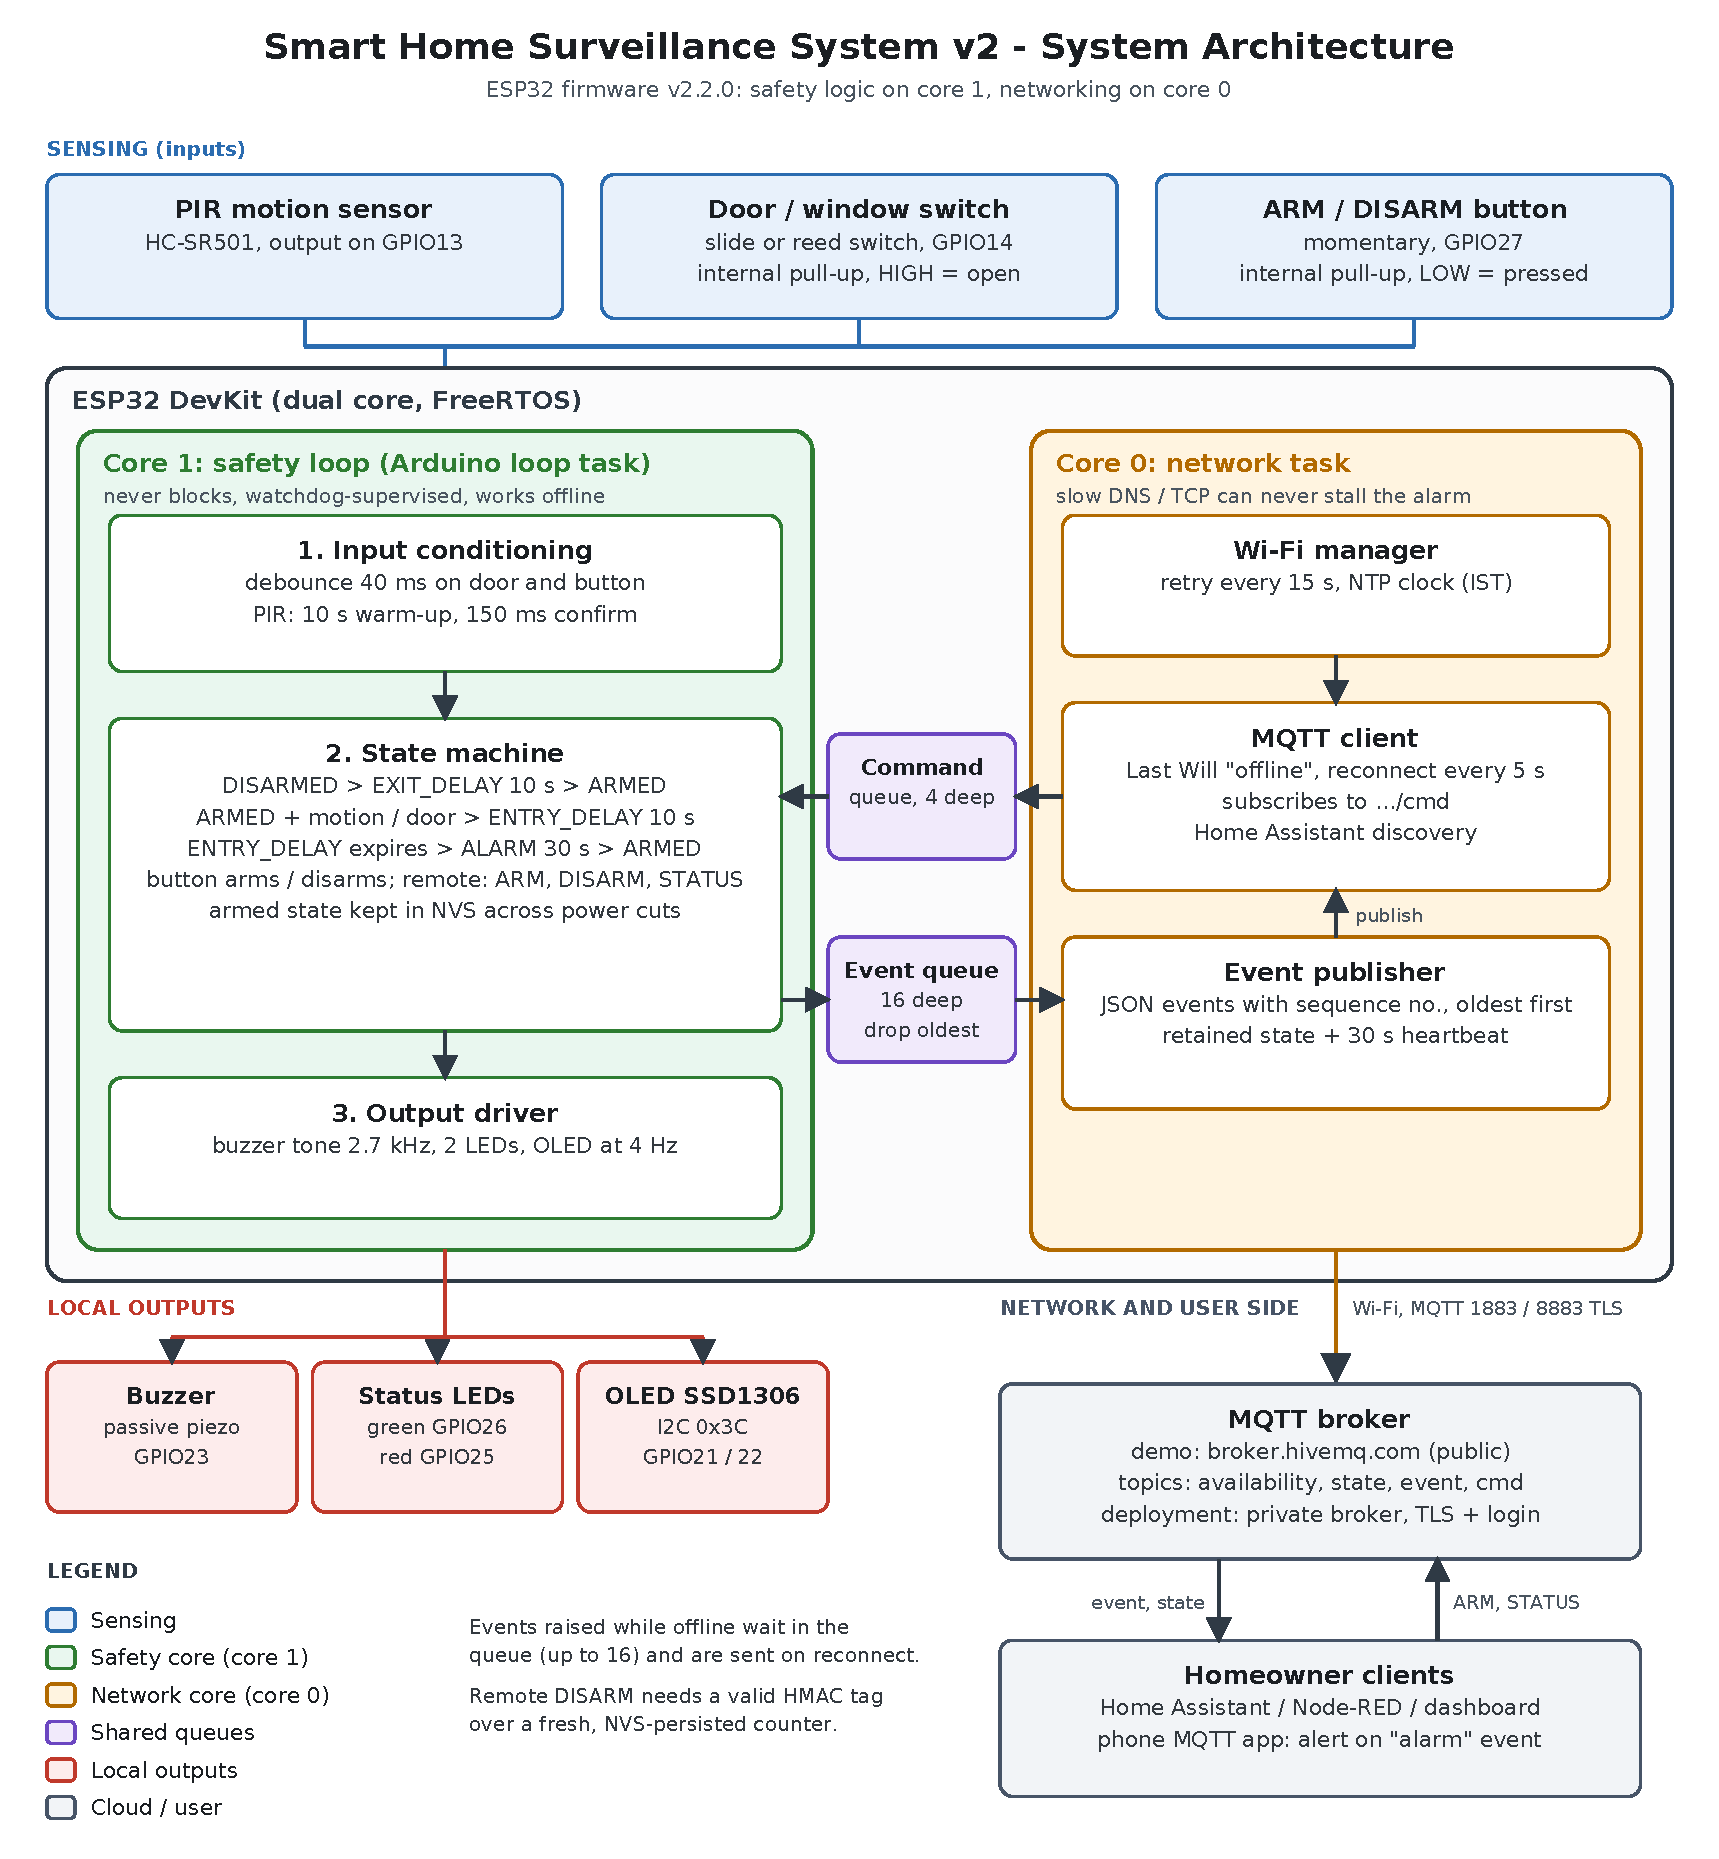
\includegraphics[width=0.96\textwidth,height=0.78\textheight,keepaspectratio]{architecture.pdf}
\caption[System architecture]{System architecture. The safety domain on core~1 (green) and the
network domain on core~0 (blue) communicate only through two bounded queues and one
mutex-guarded status snapshot. Every pin number, timeout and queue depth shown is transcribed
from \code{firmware/smart\_home/smart\_home.ino}.}
\label{fig:arch}
\end{figure}

\section{Hardware platform}

The device is an ESP32-WROOM-32 development board. The relevant properties are that it is
dual-core — two Xtensa LX6 cores — and that its 802.11 radio shares the die with them. A
single-core variant such as the ESP32-C3 cannot host this architecture at all, which is why
Appendix~\ref{app:hardware} insists on the dual-core part for the measurement.

\begin{longtable}{@{}p{0.22\textwidth}p{0.13\textwidth}p{0.57\textwidth}@{}}
\toprule
\textbf{Peripheral} & \textbf{Pin} & \textbf{Role} \\
\midrule
\endhead
PIR motion sensor (HC-SR501)  & GPIO 13 & Primary intrusion detector; 10\,s warm-up and a
150\,ms confirmation window \\
Door or window switch         & GPIO 14 & Reed or slide switch, internal pull-up, HIGH when
open \\
Arm/disarm button             & GPIO 27 & Momentary, internal pull-up, LOW when pressed,
40\,ms debounce \\
Siren (passive piezo)         & GPIO 23 & Driven at 2.7\,kHz \\
Armed indicator               & GPIO 26 & Green \\
Alarm indicator               & GPIO 25 & Red \\
OLED display (SSD1306)        & GPIO 21, 22 & I2C at address \code{0x3C}, refreshed every
250\,ms \\
\bottomrule
\end{longtable}

\section{Core 1: the safety domain}

Core 1 hosts the Arduino \code{loop()} task, which is the safety function. It performs three
stages in sequence on every pass.

\begin{enumerate}[leftmargin=1.8em,itemsep=4pt]
  \item \textbf{Input conditioning.} Sensor lines are sampled and debounced. The PIR is
        suppressed for 10\,s after power-up, because the HC-SR501 produces spurious output
        while stabilising, and a motion indication must persist for 150\,ms before it is
        treated as real.
  \item \textbf{State machine.} The conditioned inputs and any dequeued command advance a
        five-state machine. The armed state is written to non-volatile storage so that a power
        interruption does not disarm the system.
  \item \textbf{Output driver.} The siren, the two indicators and the display are driven from
        the current state.
\end{enumerate}

Two properties of this loop matter more than its contents. It \emph{never blocks}: every
acquisition of a shared resource uses a zero timeout and proceeds without it on failure. And it
is \emph{independent of the network}: with the radio disabled, every function in
Section~\ref{ch:req}'s FR1 to FR6 still works.

\subsection{The state machine}

\begin{longtable}{@{}p{0.17\textwidth}p{0.13\textwidth}p{0.62\textwidth}@{}}
\toprule
\textbf{State} & \textbf{Duration} & \textbf{Meaning and exits} \\
\midrule
\endhead
\code{DISARMED}    & ---     & Sensors are ignored. Exits on a local button press or an
authenticated \code{ARM}/\code{ARM\_AWAY}. \\
\code{EXIT\_DELAY} & 10\,s   & The occupant is leaving. Exits to \code{ARMED} on expiry. \\
\code{ARMED}       & ---     & Sensors are live. Motion or a door opening moves to
\code{ENTRY\_DELAY}. \\
\code{ENTRY\_DELAY}& 10\,s   & Grace period for a legitimate entry. A disarm here returns to
\code{DISARMED}; expiry moves to \code{ALARM}. \\
\code{ALARM}       & 30\,s   & The siren sounds. Returns to \code{ARMED} on expiry. \\
\bottomrule
\end{longtable}

\section{Core 0: the network domain}

Core 0 hosts a single FreeRTOS task created explicitly rather than by the framework:

\begin{lstlisting}[style=cpp,caption={Network task creation, \code{smart\_home.ino}},
                   label={lst:taskcreate}]
xTaskCreatePinnedToCore(networkTask, "net", 8192, nullptr, 1, nullptr, 0);
\end{lstlisting}

The final argument pins the task to core~0. The Arduino \code{loop()} runs on core~1 by
default, so the two domains are on separate cores without any further configuration. The task
performs Wi-Fi management, the MQTT client, and event publication.

\begin{itemize}[leftmargin=1.6em,itemsep=4pt]
  \item \textbf{Wi-Fi manager.} Reconnects every 15\,s on loss, and maintains an NTP-corrected
        clock for event timestamps.
  \item \textbf{MQTT client.} Reconnects every 5\,s, registers a Last Will message so the
        broker announces the device as offline, subscribes to the command topic and publishes
        Home Assistant discovery metadata.
  \item \textbf{Event publisher.} Publishes JSON events carrying a sequence number, oldest
        first, together with a retained state topic and a 30\,s heartbeat.
\end{itemize}

Every one of these operations can block for a long time. DNS resolution, TCP connection
establishment and the TLS handshake are all unbounded in the worst case. That is precisely why
they are on the other core.

\section{What the two domains share}

Exactly three objects cross the boundary, and the discipline applied to each is what the
isolation argument rests on.

\begin{longtable}{@{}p{0.20\textwidth}p{0.11\textwidth}p{0.61\textwidth}@{}}
\toprule
\textbf{Object} & \textbf{Bound} & \textbf{Discipline} \\
\midrule
\endhead
Command queue \code{cmdQ}  & 4 entries  & Core 0 enqueues non-blocking; core 1 drains at most
\code{CMD\_DRAIN\_PER\_PASS} entries per pass. \\
Event queue \code{eventQ}  & 16 entries & Core 1 enqueues non-blocking; the oldest entry is
dropped when full, so the safety loop never waits for a consumer. \\
Status snapshot            & 1 struct   & Guarded by \code{statusMutex}. Core 1 acquires with
timeout \textbf{0}; core 0 acquires with a 10\,ms timeout. Copied every 500\,ms. \\
\bottomrule
\end{longtable}

\subsection{The asymmetric mutex timeout}

The status snapshot is the mechanism most easily overlooked and it is the heart of the design.
Both cores need access to the same state structure: core~1 writes it, core~0 reads it in order
to publish. A conventional mutex would let the network core's acquisition delay the safety
core.

The firmware avoids this by making the timeouts asymmetric:

\begin{lstlisting}[style=cpp,caption={Asymmetric acquisition, \code{smart\_home.ino}},
                   label={lst:mutex}]
/* core 1, the safety loop: never waits */
if (xSemaphoreTake(statusMutex, 0) == pdTRUE) {
    /* copy the snapshot */
    xSemaphoreGive(statusMutex);
}
/* if the lock was unavailable, the loop simply continues; the snapshot
   is refreshed on the next pass 500 ms later */

/* core 0, the network task: may wait up to 10 ms */
if (xSemaphoreTake(statusMutex, pdMS_TO_TICKS(10)) == pdTRUE) {
    /* read the snapshot and publish */
    xSemaphoreGive(statusMutex);
}
\end{lstlisting}

The consequence is that the blocking term in the response-time analysis of
Section~\ref{sec:impl-rt} is \emph{identically zero by construction} rather than merely small.
The safety loop cannot be made to wait, because it never asks to. The cost is that a status
publication may occasionally carry a snapshot up to 500\,ms old, which is an acceptable price
for a telemetry path and an unacceptable one for a safety path — which is why the asymmetry runs
in this direction and not the other.

\section{The command path}

Figure~\ref{fig:cmdflow} shows the full path a remote command takes, and which core performs
each stage.

\begin{figure}[htbp]
\centering
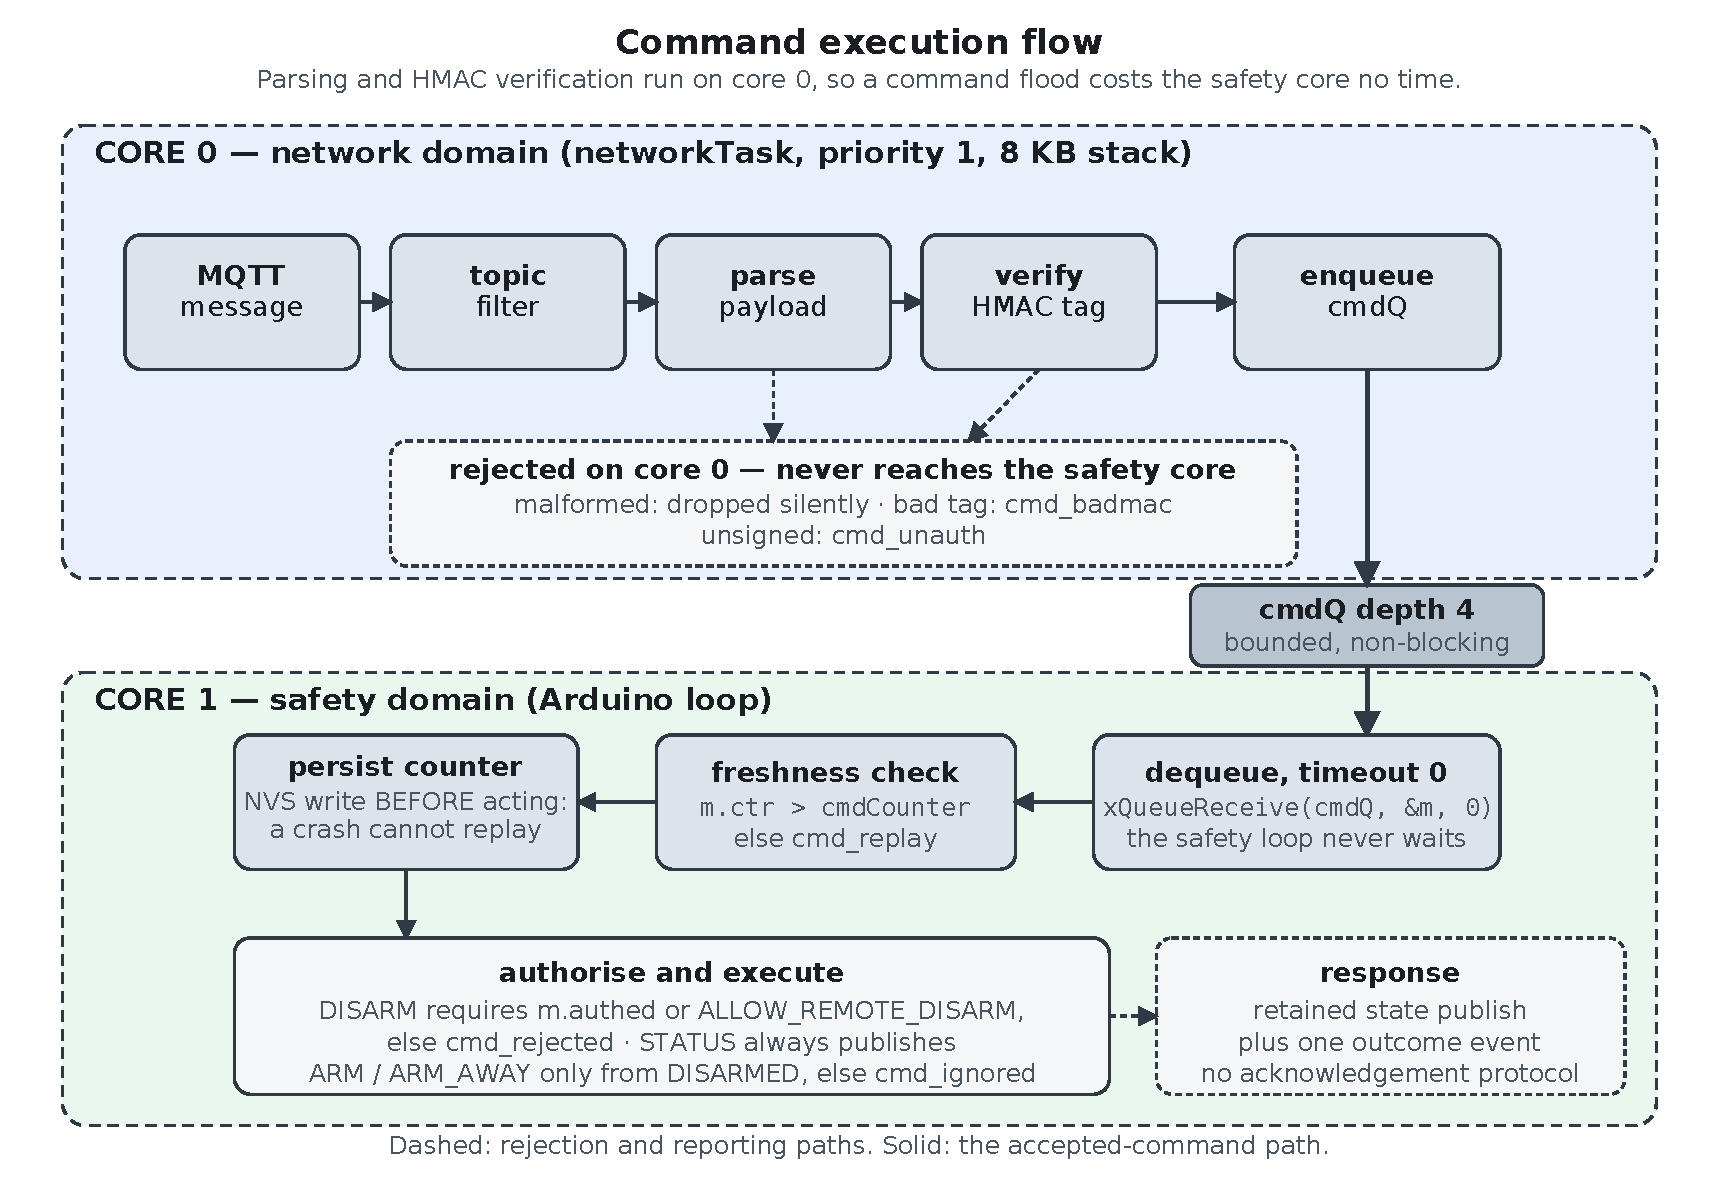
\includegraphics[width=\textwidth]{command_flow.pdf}
\caption[Command execution flow]{Command execution flow. Parsing and verification complete on
core~0; the replay counter is committed to non-volatile storage before the command is acted on.
Rejected commands never reach the safety core.}
\label{fig:cmdflow}
\end{figure}

The ordering is deliberate. All parsing, all cryptographic verification and all rejection happen
on core~0. A malformed, unsigned or incorrectly signed command is discarded there and never
occupies a queue slot. Only a verified command is enqueued, so the safety core's work per
command is bounded and small.

The wire format is deliberately minimal:
\[
\texttt{VERB}:\texttt{CTR}:\mathrm{hex}\bigl(\mathrm{HMAC\text{-}SHA256}(k,\ \texttt{"VERB:CTR"})[0{:}16]\bigr)
\]
A verb, a counter, and a 128-bit truncated tag over both. The tag covers the counter, so an
adversary cannot replay a captured command with a higher counter.

\section{Security architecture}

Three layers are available, and Chapter~\ref{ch:security} reports what each does and does not
contain. Figure~\ref{fig:aclarch} shows the broker-side permissions.

\begin{figure}[htbp]
\centering
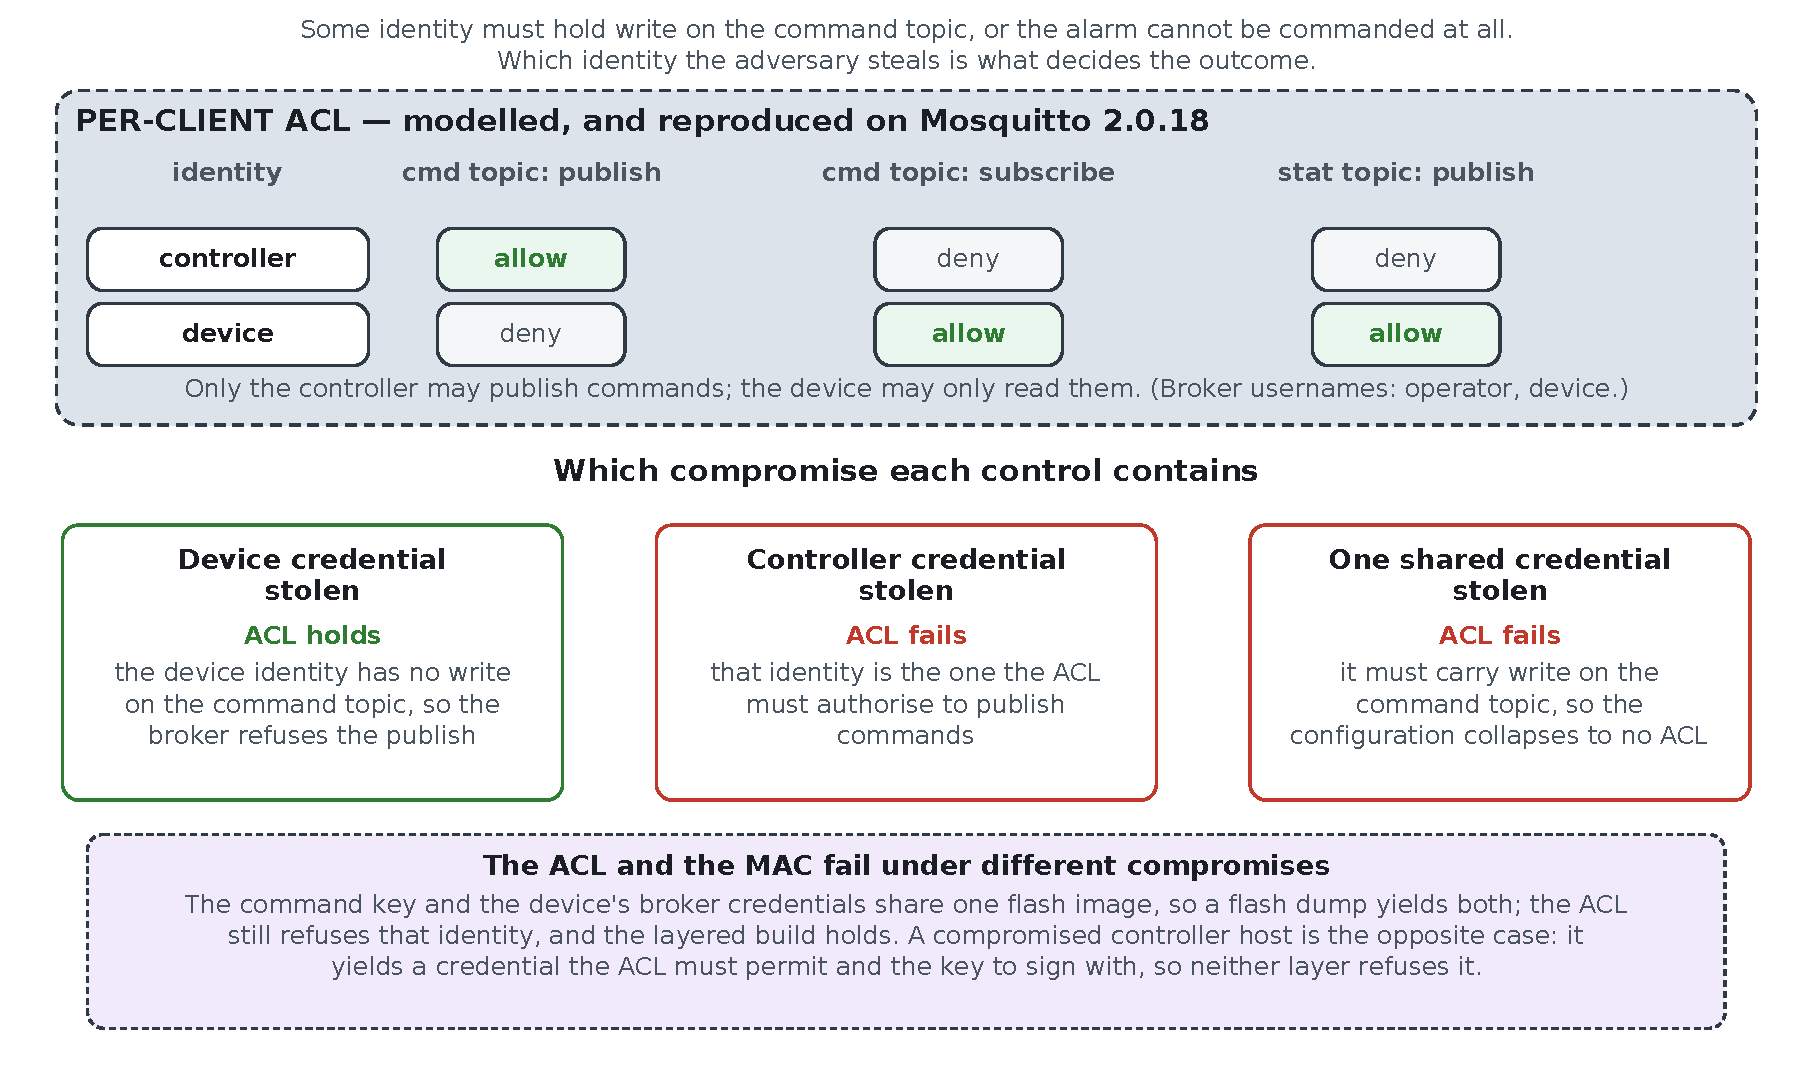
\includegraphics[width=\textwidth]{acl_architecture.pdf}
\caption[Broker access control architecture]{Per-client topic permissions, and which compromise
each control contains. The matrix is both the configuration the ablation models and the
Mosquitto \code{acl\_file} used in the broker experiment.}
\label{fig:aclarch}
\end{figure}

\begin{enumerate}[leftmargin=1.8em,itemsep=5pt]
  \item \textbf{Transport: TLS.} Protects each hop. Does not survive the broker, because the
        broker terminates the connection and re-originates the message.
  \item \textbf{Broker authorisation: per-client credentials and a deny-by-default access
        control list.} The controller identity may publish on the command topic; the device
        identity may only read it. This contains a compromised \emph{device} credential and
        cannot contain a compromised \emph{controller} credential, because the list must permit
        that identity to publish.
  \item \textbf{Application layer: HMAC-SHA256 over a monotonic counter.} Survives any broker
        credential compromise on its own, and falls only when the key itself is compromised.
\end{enumerate}

The counter is persisted to non-volatile storage \emph{before} the command is acted on, not
after. Committing afterwards would leave a window in which a power interruption between action
and commit permits a replay.

\section{Operator and controller interactions}

Three parties exist in the deployed system, and their separation is what the access control list
encodes.

\begin{itemize}[leftmargin=1.6em,itemsep=4pt]
  \item \textbf{The device} subscribes to the command topic and publishes state and events. In
        the broker configuration its username is \code{device}.
  \item \textbf{The controller} — a phone application, Home Assistant or Node-RED — publishes
        commands and reads state. Its username is \code{operator}. It is the identity the access
        control list must authorise to publish, which is why its compromise is scenario~E$'$.
  \item \textbf{The broker} mediates. In the default configuration this is a public test broker;
        the evaluation used a private Mosquitto instance with TLS, per-client credentials and
        the access control list shown in Figure~\ref{fig:aclarch}.
\end{itemize}

\section{What the architecture does not contain}

Stated explicitly, so the diagram is not read as claiming more than it shows.

\begin{itemize}[leftmargin=1.6em,itemsep=4pt]
  \item \textbf{No secure element and no hardware key storage.} The command key is in the flash
        image. This is why a flash dump yields it, and why scenario E exists.
  \item \textbf{No secure boot and no flash encryption.} Both are available on the ESP32 and
        neither is enabled in the artefact studied.
  \item \textbf{No over-the-air update path.} A deployed device would need one; its absence
        removes an attack surface and a capability at the same time.
  \item \textbf{No key rotation or provisioning protocol.} Out of scope, as
        Section~\ref{ch:req} states.
  \item \textbf{No redundant sensing or watchdog escalation beyond the framework default.}
\end{itemize}

\chapter{Technologies, Tools and Development Environment}\label{ch:tools}

Every version in this chapter was read from the tool itself in the environment that produced
the committed results. Where a version could not be verified, that is stated rather than
guessed.

\section{Target platform}

\begin{longtable}{@{}p{0.23\textwidth}p{0.16\textwidth}p{0.55\textwidth}@{}}
\toprule
\textbf{Item} & \textbf{Version} & \textbf{Role and why} \\
\midrule
\endhead
ESP32-WROOM-32 & DevKit v1 & The artefact under study. Chosen because it is the platform the
research question is about: dual-core, with the radio on the same die. \\
Xtensa LX6 cores & 2 cores & Core affinity is the only isolation primitive available; the
whole architecture depends on there being two. \\
arduino-esp32 & 2.0.17 and 3.3.12 & Both evaluated, because the buzzer driver API changed
between them and the firmware must build under each. Resource cost is reported for both
(Table~\ref{tab:rep-build}). \\
FreeRTOS & as shipped with the above & Supplies \code{xTaskCreatePinnedToCore}, queues and
semaphores. No version independent of the framework is pinned. \\
\bottomrule
\end{longtable}

\subsection{Firmware dependencies}

\begin{longtable}{@{}p{0.30\textwidth}p{0.62\textwidth}@{}}
\toprule
\textbf{Library} & \textbf{Purpose in this firmware} \\
\midrule
\endhead
\code{PubSubClient}            & MQTT 3.1.1 client: connection, subscription, publication,
Last Will \\
\code{WiFiClientSecure}        & TLS transport to the broker \\
\code{Adafruit\_SSD1306}, \code{Adafruit\_GFX} & Local OLED status display \\
\code{Preferences}             & Non-volatile storage for the armed state and the replay
counter \\
\code{mbedtls} (via the SDK)   & HMAC-SHA256 for command authentication \\
\bottomrule
\end{longtable}

\section{Verification and experimentation environment}

This is a separate environment from the target, and the distinction is material: every result
reported in Chapter~\ref{ch:results} except the broker experiment was produced here, on a host,
and not on the device.

\begin{longtable}{@{}p{0.21\textwidth}p{0.17\textwidth}p{0.56\textwidth}@{}}
\toprule
\textbf{Tool} & \textbf{Version} & \textbf{Role and where it appears} \\
\midrule
\endhead
GCC / g++ & 13.3.0 & Compiles the firmware logic against host stubs, and the harnesses in
\code{experiments/*.cpp}. Also supplies AddressSanitizer and UndefinedBehaviorSanitizer for
the fuzzing campaign. \\
Python & 3.13.18 & All analysis, figure generation and verification scripts. Statistics are
implemented with the standard library only, so no external package can alter a reported
value. \\
TLA+ / TLC & TLC2 2026.10.24.013619 (rev \code{2ef2af8}) & Exhaustive model checking of
\code{formal/AlarmFSM.tla} and \code{formal/Isolation.tla}, and of the deliberately defective
configuration that must fail. \\
Java & OpenJDK, as installed & Runtime for \code{tla2tools.jar} (4{,}502{,}259 bytes,
committed). \\
Mosquitto & 2.0.18 & The live broker for experiment E6. The only component in the evaluation
that is external software observed rather than simulated. \\
\code{mosquitto\_passwd} & with 2.0.18 & Generates the password file for per-client
authentication. \\
OpenSSL & as installed & Generates the private certificate authority and server certificate
for the broker testbed. \\
matplotlib & 3.11.2 & Figures 3 and 5. Configured through \code{experiments/figstyle.py} with
\code{pdf.fonttype~42}, so TrueType fonts are embedded rather than Type~3. \\
cairosvg & current at build & Converts the generated SVG diagrams to PDF and PNG. \\
Pillow & current at build & Measures text in the real font for the figure-fit check. \\
pdflatex & \TeX\ Live 2024 & Builds the manuscript and this report. \\
Pandoc & 3.1.3 & Produces the editable DOCX of this report. \\
Git & as installed & Version control; the commit hash on the title page identifies the exact
state. \\
GitHub Actions & --- & Continuous integration: re-runs the formal verification and a reduced
adversarial campaign on every push. \\
\bottomrule
\end{longtable}

\subsection{Why the firmware is tested against host stubs}

The firmware logic is compiled for the host against a set of stub headers in
\code{tests/host/stubs/}, which provide the Arduino, FreeRTOS, \code{WiFi}, \code{PubSubClient},
\code{Preferences}, \code{Wire} and display interfaces.

The reason is throughput. A campaign of 9,600 adversarial trials and 3,000,000 fuzzing
iterations is not feasible on the device at any useful speed, and the sanitizers that make the
fuzzing meaningful do not exist for the Xtensa target. Compiling for the host makes both
possible.

The cost is equally clear and is stated wherever a result from this environment is reported:
\textbf{the host harness advances a logical clock}. There is no radio, no true parallel
execution and no contention for shared silicon. Latency variance in this environment is
identically zero, which is why no timing conclusion is drawn from it anywhere in this report.

The firmware logic itself is \emph{not} modified for testing. The same \code{smart\_home.ino} is
compiled; only the headers it includes differ.

\section{Resource cost on the target}

Measured at build time by the Arduino toolchain, for the two framework versions. This is the one
measurement in the project taken by real tooling on the real target, and it describes the binary
rather than the running device.

\begin{table}[htbp]
\centering
\caption[Firmware resource cost]{Firmware resource cost, measured at build time.}
\label{tab:rep-build}
\begin{tabular}{@{}lrrrr@{}}
\toprule
Framework version & Flash (B) & of budget & RAM (B) & of budget \\
\midrule
arduino-esp32 2.0.17 & 793{,}433 & 60.5\% & 46{,}372 & 14.2\% \\
arduino-esp32 3.3.12 & 968{,}221 & 73.9\% & 49{,}876 & 15.2\% \\
\bottomrule
\end{tabular}
\end{table}

The increase under the newer framework is substantial — roughly 175\,kB of flash — and is a
property of the framework rather than of this firmware. It is reported because a reader
reproducing the build will see one figure or the other depending on which version they install.

\section{Simulation and modelling tools}

\begin{longtable}{@{}p{0.31\textwidth}p{0.61\textwidth}@{}}
\toprule
\textbf{Tool} & \textbf{Role} \\
\midrule
\endhead
Wokwi (\code{wokwi/diagram.json}) & Circuit definition for browser-based simulation of the
peripherals. Used during development for wiring verification; \textbf{no reported result comes
from it}. \\
\code{experiments/ablation.cpp} & The twelve-configuration harness. Models broker admission and
access control in \code{deliverGuarded}/\code{admit}. \\
\code{experiments/campaign.cpp} & The adversarial campaign harness, E1 and E2. \\
\code{experiments/fuzz\_cmd.cpp} & The command-parser fuzzer, run under both sanitizers. \\
\code{experiments/sensitivity.cpp} & The detector parameter sweep. \\
\bottomrule
\end{longtable}

\section{Code quality and verification infrastructure}

A deliberate choice was made to treat the verification infrastructure as part of the artefact
rather than as scaffolding, because four defects were found \emph{in the harnesses themselves}
during this work — two of which produced results that flattered the intended conclusion.

\begin{longtable}{@{}p{0.32\textwidth}p{0.60\textwidth}@{}}
\toprule
\textbf{Check} & \textbf{What it prevents} \\
\midrule
\endhead
\code{tests/host/run\_tests.sh} & 129 assertions over the firmware logic, including three
negative build-guard tests that require a defective configuration to fail to compile \\
\code{formal/run\_tlc.sh} & Three model-checking configurations; the third \emph{must} report a
violation, so a vacuous invariant cannot recur silently \\
\code{experiments/test\_conformance.py} & 19,529 firmware transitions checked against the
specification's transition relation, with a negative control \\
\code{experiments/test\_harness.py} & Metamorphic and differential properties of the harness:
determinism, seed sensitivity, monotone attack effort, mode separation, and agreement of the
HMAC payload format with an independent implementation \\
\code{experiments/corpus/test\_rule.py} & Eight controls for the static rule, including this
project's own pre-repair guard \\
\code{experiments/validate\_figures.py} & Recomputes every plotted value from the raw per-trial
records, not from the derived summary \\
\code{experiments/check\_figure\_type.py} & Fails the build if any figure label would print
below 6\,pt \\
\code{experiments/check\_figure\_fit.py} & Measures every label in the real font and fails on
clipping \\
\bottomrule
\end{longtable}

The last two exist because a defect was found that visual inspection cannot detect: every
diagram in an earlier revision printed its smallest label at roughly 4\,pt, which is a function
of the canvas width and the figure's scale factor rather than anything visible on screen.

\section{What the environment could not do}

Recorded here so that no reader infers a capability that did not exist.

\begin{itemize}[leftmargin=1.6em,itemsep=4pt]
  \item \textbf{No physical ESP32 hardware} was available in the environment that produced
        these results. There were no serial devices, no USB, no \code{arduino-cli} and no
        wireless interface. Appendix~\ref{app:hardware} records the probe that established
        this.
  \item \textbf{No RF-shielded enclosure}, which is a hard prerequisite for the radio-layer
        condition.
  \item \textbf{No licensed similarity-checking tool.}
  \item \textbf{No institutional access} to Scopus or Journal Citation Reports, which is why no
        journal quartile is asserted anywhere in this work.
\end{itemize}

\chapter{Detailed Implementation}\label{ch:impl}

This chapter explains the implementation at the level of individual functions and the reasoning
behind them. Every excerpt is quoted from the committed source and the file and function are
named, so a reader can open the original. The complete source is supplied separately as
\code{COMPLETE\_SOURCE\_CODE\_AND\_EXPERIMENTS.zip}; the inventory is
Appendix~\ref{app:inventory}.

Three sections carry more weight than the rest and are the ones to read if time is short:
Section~\ref{sec:impl-cmd} on the command path, Section~\ref{sec:impl-guard} on the
configuration guard, and Section~\ref{sec:impl-drain} on the unbounded drain.

\section{Module map}

\begin{longtable}{@{}p{0.31\textwidth}p{0.61\textwidth}@{}}
\toprule
\textbf{File} & \textbf{Responsibility} \\
\midrule
\endhead
\code{smart\_home.ino} & The artefact under study. Pin definitions, timing constants, build
guards, the state machine, both cores' tasks, and the command path. 713 lines of code. \\
\code{authmac.h} & HMAC-SHA256 command authentication: tag computation and constant-time
comparison \\
\code{alertmsg.h} & Event record structure and serialisation \\
\code{wifi_guard.h} & Deauthentication frame counting and the detector threshold \\
\code{sensor_fusion.h} & Optional PIR and radar fusion; off in the evaluated configuration \\
\code{secrets.example.h} & Template for credentials and keys. The demo key it carries is
public by design, and the build refuses to use it with authentication enabled \\
\bottomrule
\end{longtable}

\section{Constants and the build configuration}

All timing and pin constants are \code{constexpr}, in one block, so that a reader auditing the
firmware's temporal behaviour can find every value in one place.

\begin{lstlisting}[style=cpp,caption={Timing constants, \code{smart\_home.ino}}]
constexpr uint32_t EXIT_DELAY_MS      = 10000;  // time to leave after pressing ARM
constexpr uint32_t ENTRY_DELAY_MS     = 10000;  // time to disarm after a trigger
constexpr uint32_t ALARM_DURATION_MS  = 30000;  // siren length, then system re-arms
constexpr uint32_t PIR_WARMUP_MS      = 10000;  // suits the simulator; 60000 on a real HC-SR501
constexpr uint32_t PIR_CONFIRM_MS     = 150;    // PIR must stay HIGH this long
constexpr uint32_t DEBOUNCE_MS        = 40;
constexpr uint32_t OLED_REFRESH_MS    = 250;
constexpr uint32_t STATUS_COPY_MS     = 500;    // loop -> network task snapshot rate
constexpr uint32_t HEARTBEAT_MS       = 30000;
constexpr uint32_t WIFI_RETRY_MS      = 15000;
constexpr uint32_t MQTT_RETRY_MS      = 5000;
\end{lstlisting}

\code{PIR\_WARMUP\_MS} carries a comment rather than a single value because the correct number
differs between the simulator and the physical sensor. Recording that in the source is
preferable to silently choosing one and misleading whoever deploys it.

\section{Data structures}

\begin{lstlisting}[style=cpp,caption={Core data structures, \code{smart\_home.ino}}]
enum class SysState : uint8_t { DISARMED, EXIT_DELAY, ARMED, ENTRY_DELAY, ALARM };
enum class Cmd      : uint8_t { ARM, DISARM, STATUS };

struct CmdMsg {   /* one entry in the command queue */
  Cmd      cmd;
  bool     authed;   /* the MAC verified */
  uint32_t ctr;      /* the counter carried by the command */
};
\end{lstlisting}

\code{CmdMsg} is deliberately small and contains no pointers. It is copied by value into a
FreeRTOS queue, so a command crossing the core boundary involves no shared allocation and no
lifetime question. The \code{authed} flag is set on core~0 after verification; core~1 trusts it
precisely because nothing else can write to that queue.

\section{Core 1: the safety loop}

\subsection{Input conditioning}

\code{readSensors()} samples the three input lines and applies two independent filters. The
button and the door switch are debounced over \code{DEBOUNCE\_MS}; the PIR is suppressed
entirely for \code{PIR\_WARMUP\_MS} after boot and then required to hold its indication for
\code{PIR\_CONFIRM\_MS}.

The two filters are different because the failure modes are different. A mechanical switch
chatters on contact, which debouncing addresses. A pyroelectric sensor produces spurious output
while its reference stabilises after power-up, and then occasional short pulses in normal
operation — a warm-up suppression and a confirmation window address those.

\subsection{The state machine}

\code{stepFsm()} implements the five-state machine of Chapter~\ref{ch:arch}. Its structure is a
switch on the current state, with time-based transitions compared against a stored entry
timestamp rather than counted down, so that a missed loop pass cannot lose time.

The armed state is written to non-volatile storage on every change through
\code{persistState()}, which satisfies FR6: a power interruption while armed leaves the system
armed.

\subsection{Output driving}

\code{driveOutputs()} is the only function that writes to the siren, the indicators or the
display. Concentrating output in one function means that a reader auditing when the siren can
sound has one place to look.

The buzzer driver handles an API change between arduino-esp32 2.x, which is channel-based, and
3.x, which is pin-based. The firmware supports both because both were evaluated.

\section{The command path}\label{sec:impl-cmd}

\subsection{Authentication on core 0}

The wire format is a verb, a counter and a truncated tag over both:
\[
\texttt{VERB}:\texttt{CTR}:\mathrm{hex}\bigl(\mathrm{HMAC\text{-}SHA256}(k,\ \texttt{"VERB:CTR"})[0{:}16]\bigr)
\]

Two design decisions are worth explaining. The tag is truncated to 128 bits
(\code{AUTH\_TAG\_BYTES = 16}) because a 256-bit tag in hexadecimal would double the wire
length for no practical security gain: the forgery probability against a 128-bit tag is
$2^{-128}$, which is far below any threshold that matters here. And the tag covers the
\emph{counter as well as the verb}, which is what prevents an adversary from taking a captured
command and incrementing its counter.

Comparison uses a constant-time routine in \code{authmac.h}. On a device of this kind a timing
side channel on tag comparison is a remote prospect, but constant-time comparison costs
nothing and removes the question.

\subsection{Dispatch on core 1}

\code{handleCommands()} runs on the safety core and is the only consumer of the command queue.

\begin{lstlisting}[style=cpp,caption={Command dispatch, \code{handleCommands()} in
\code{smart\_home.ino}},label={lst:handlecmd}]
static void handleCommands(uint32_t now) {
  CmdMsg m;
  for (int drained = 0;
       drained < CMD_DRAIN_PER_PASS && xQueueReceive(cmdQ, &m, 0) == pdTRUE;
       drained++) {
    // Marker from the network task for a command whose MAC did not verify.
    if (!m.authed && m.ctr == 0xFFFFFFFFu) { emitEvent("cmd_badmac", "remote"); continue; }

    if (m.authed) {
      // Reject a replay: the counter must strictly advance.
      if (m.ctr <= cmdCounter) { emitEvent("cmd_replay", "remote"); continue; }
      persistCounter(m.ctr);
    }
#if AUTH_COMMANDS
    else {
      // Authentication is required but this command was unsigned.
      emitEvent("cmd_unauth", "remote");
      continue;
    }
#endif
    const char* src = m.authed ? "remote_auth" : "remote";
    switch (m.cmd) {
      case Cmd::ARM:
        if (state == SysState::DISARMED) beginArm(src, now);
        else emitEvent("cmd_ignored", src);
        break;
      case Cmd::DISARM:
        if (m.authed || ALLOW_REMOTE_DISARM) {
          if (state != SysState::DISARMED) disarm(src, now);
          else emitEvent("cmd_ignored", src);
        } else {
          emitEvent("cmd_rejected", src);
        }
        break;
      case Cmd::STATUS:
        statusDirty = true;
        break;
    }
  }
}
\end{lstlisting}

Reading this block by block:

\begin{description}[leftmargin=1.6em,itemsep=4pt]
  \item[The loop header] is the bounded drain discussed in Section~\ref{sec:impl-drain}. The
        \code{0} timeout on \code{xQueueReceive} means the safety loop never waits for a
        command.
  \item[The \code{cmd\_badmac} marker] is how core~0 reports a verification failure without
        performing any dispatch itself. The sentinel counter \code{0xFFFFFFFF} distinguishes it
        from a genuine unsigned command.
  \item[The replay check] requires the counter to \emph{strictly} advance, and
        \code{persistCounter()} commits the new value \emph{before} the command is acted on.
        Committing afterwards would leave a window in which a power interruption between
        action and commit permits the same command to be replayed.
  \item[The \code{AUTH\_COMMANDS} branch] is where an unsigned command is refused when
        authentication is required. This is the clause the configuration guard of
        Section~\ref{sec:impl-guard} is supposed to protect.
  \item[The \code{DISARM} case] is the one that matters for security. A validly signed command
        proves the key holder sent it, so disarm is safe irrespective of
        \code{ALLOW\_REMOTE\_DISARM}. The disjunction exists for a deployment that uses TLS and
        a broker login without command signing — and the soundness of \emph{that} configuration
        is exactly what this project found to be unjustified.
  \item[\code{cmd\_ignored} versus \code{cmd\_rejected}] are distinguished deliberately: the
        first means a well-authorised command that does not apply in the current state, the
        second means a command that was not authorised. Conflating them would make the event
        log useless for exactly the analysis this project performed.
\end{description}

\section{The configuration guard}\label{sec:impl-guard}

\subsection{The defect}

The original guard permitted \code{ALLOW\_REMOTE\_DISARM} without \code{AUTH\_COMMANDS}
provided that TLS and a broker login were configured. The reasoning was that a deployment with
transport security and broker authentication has established who may publish.

The reasoning is unsound, and it is unsound for a structural reason rather than through an
oversight in the code. The broker terminates each client's TLS connection and re-originates
every message it forwards, so an arriving command carries no evidence of which client published
it. \code{MQTT\_HAS\_LOGIN} describes \emph{this device's own build}, not any publisher's
authority. One leaked credential — any credential permitted to publish on the command topic —
is therefore sufficient to disarm the alarm, and the guard compiled such a build without
complaint.

\subsection{The repair}

\begin{lstlisting}[style=cpp,caption={The corrected guard, \code{smart\_home.ino}},
                   label={lst:guard}]
#if ALLOW_REMOTE_DISARM && !AUTH_COMMANDS && !defined(ACKNOWLEDGE_UNAUTHENTICATED_DISARM)
#  error "ALLOW_REMOTE_DISARM without AUTH_COMMANDS 1 permits anyone who can publish to the \
command topic to switch the alarm off, and TLS plus a broker login does not prevent it (see \
docs/SECURITY_ANALYSIS.md). Set AUTH_COMMANDS 1, or define \
ACKNOWLEDGE_UNAUTHENTICATED_DISARM to accept that risk deliberately."
#endif
\end{lstlisting}

The repair removes the unsound inference rather than adding a mechanism. The transport test is
gone; what remains is a requirement for either command signing or an explicit acknowledgement
that the risk is being accepted. The latter exists because the research baseline must be able
to build the defective configuration in order to measure it — and it must do so deliberately.

Figure~\ref{fig:guard} shows both versions of the decision.

\begin{figure}[htbp]
\centering
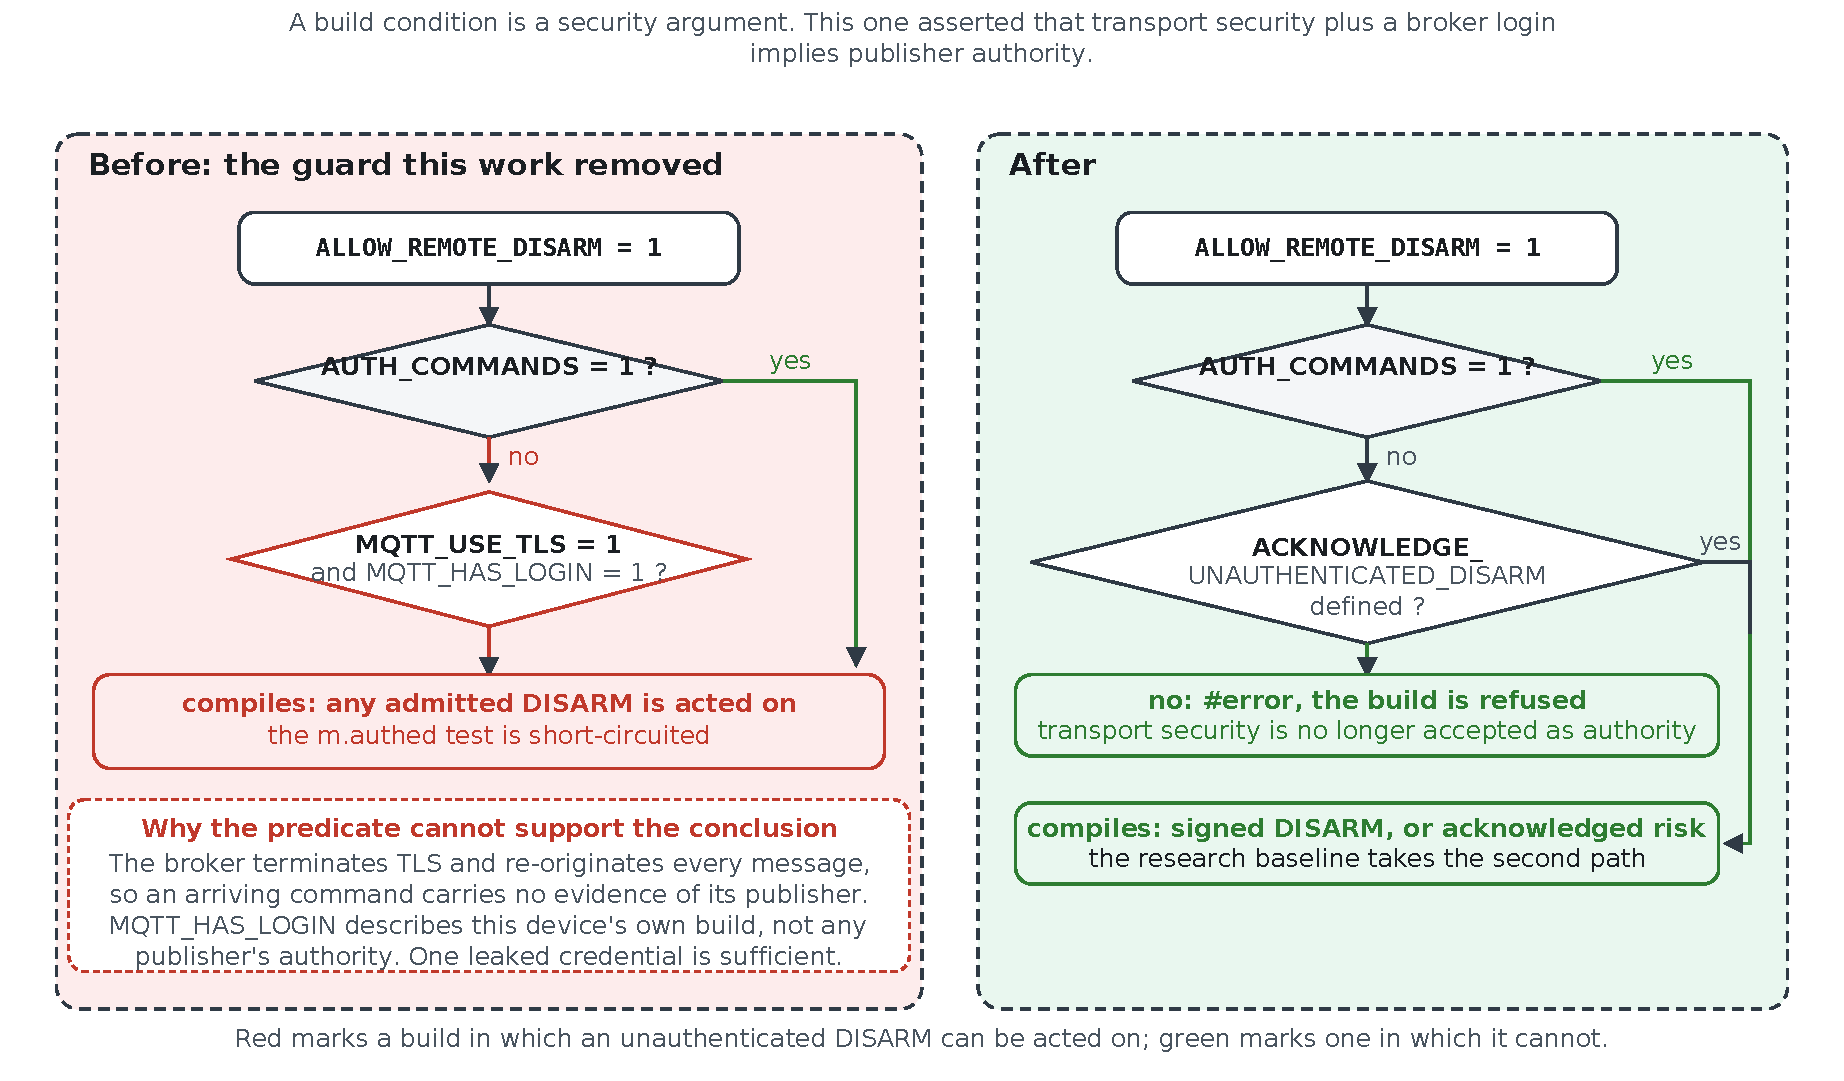
\includegraphics[width=\textwidth]{guard_decision.pdf}
\caption[Compile-guard comparison]{The defective guard and its repair, transcribed from the
preprocessor conditions. Both branches of the original reach the same outcome, which is the
defect: a signed build reaches it legitimately and an unsigned one through the unsound
transport test.}
\label{fig:guard}
\end{figure}

\subsection{A second guard: the published demo key}

A related defect was found and closed at the same time. The repository ships a
\code{secrets.example.h} whose demo command key is public by design. A build enabling
\code{AUTH\_COMMANDS} without replacing it would log every command as authenticated while any
reader of the repository could forge one.

\begin{lstlisting}[style=cpp,caption={Refusing the published key, \code{smart\_home.ino}}]
#if AUTH_COMMANDS && CMD_KEY_IS_DEMO
#  error "AUTH_COMMANDS 1 requires a real SECRET_CMD_KEY in secrets.h. The fallback key is \
published in this repository, so a command signed with it is forgeable by any reader."
#endif
\end{lstlisting}

Authentication that verifies against a published key is not authentication. The build now
refuses rather than producing a binary that reports false assurance.

\section{Response-time analysis and the unbounded drain}\label{sec:impl-rt}

\subsection{The decomposition}

The response time of the safety loop decomposes into the loop's own execution, interference
from the network core, blocking on shared resources, and residual hardware contention. Three of
the four are settled by construction.

\begin{description}[leftmargin=1.8em,itemsep=4pt]
  \item[Blocking is identically zero.] The safety loop acquires the status mutex with timeout
        \code{0} and proceeds without it on failure (Listing~\ref{lst:mutex}). It never waits,
        so no priority inversion and no blocking term exists.
  \item[Queue interference is bounded.] Both queues are bounded, both enqueues are
        non-blocking, and the event queue drops its oldest entry when full rather than making
        the producer wait.
  \item[Scheduling interference is bounded by core affinity.] The network task is pinned to
        core~0 and the safety loop runs on core~1, so the network task cannot be scheduled
        ahead of the safety loop.
  \item[Residual hardware contention cannot be settled analytically.] Contention for the
        memory bus, the caches and the interrupt controller remains, and it depends on the
        silicon and on a closed-source radio driver. This is the single composite term that
        requires measurement, and it is why Appendix~\ref{app:hardware} exists.
\end{description}

\subsection{The defect the analysis exposed}\label{sec:impl-drain}

Performing that decomposition revealed something the author had not been looking for. The
command drain was an unbounded loop:

\begin{lstlisting}[style=cpp,caption={The defective drain, before the repair}]
/* BEFORE -- no static bound on the loop's own execution time */
while (xQueueReceive(cmdQ, &m, 0) == pdTRUE) {
    /* ... dispatch ... */
}
\end{lstlisting}

The safety loop therefore had no static bound on its own execution time. Core~0 can enqueue
while core~1 dequeues, and in the default build — with \code{AUTH\_COMMANDS} disabled —
enqueueing costs only a parse, with no HMAC computation to throttle the producer. The loop
would still terminate in practice, but only through a probabilistic argument about relative
costs. That is not an acceptable basis for the one code path whose timing the entire design
exists to protect.

\begin{lstlisting}[style=cpp,caption={The repaired bound and its assertions,
\code{smart\_home.ino}},label={lst:drain}]
// Capacity of the command queue, and the bound on how many are drained per loop pass.
static constexpr int CMD_Q_LEN = 4;

// The bound equals the queue capacity, so a full queue still drains in a single pass;
// anything arriving during the pass waits for the next one, at most one loop period.
static constexpr int CMD_DRAIN_PER_PASS = CMD_Q_LEN;

static_assert(CMD_DRAIN_PER_PASS == CMD_Q_LEN,
              "the per-pass drain bound must equal the command queue capacity: smaller leaves "
              "work queued for an unbounded number of passes, larger makes the loop's worst "
              "case depend on arrival rate again");
static_assert(CMD_DRAIN_PER_PASS > 0, "a non-positive drain bound would never dequeue");
\end{lstlisting}

The bound equals the queue capacity, which is the only value that works: a smaller bound leaves
work queued for an unbounded number of passes, and a larger one makes the loop's worst case
depend on arrival rate again — reintroducing the original defect. The two static assertions
exist because deriving one constant from the other is not sufficient protection: a later change
could redefine either independently, and the response-time bound holds only while the
relationship between them does. Asserting the relationship is preferable to trusting a comment.

\subsection{Why this defect is the most instructive result in the project}

The unbounded drain had survived:

\begin{itemize}[leftmargin=1.6em,itemsep=3pt]
  \item 129 host tests;
  \item 3,000,000 fuzzing iterations under AddressSanitizer and UndefinedBehaviorSanitizer;
  \item 9,600 adversarial trials, including sustained flooding at up to 20,000 messages per
        second;
  \item exhaustive model checking of both specifications.
\end{itemize}

Every one of those techniques exercises a \emph{running system}, and in every execution the loop
terminated. None of them asks whether the loop's termination is \emph{bounded}, because that is
a question about the program's design rather than about any particular execution. An analytical
method costing an afternoon found what several million executions did not.

\section{The network task}

\code{networkTask()} is a conventional reconnect loop. Its structure is a state check followed
by the appropriate action, with each retry governed by its own interval constant so that a
failing Wi-Fi connection does not cause an MQTT reconnect storm.

Error handling throughout is by \emph{omission rather than exception}: a failed publish is
retried on the next pass, a failed snapshot acquisition is skipped, and a failed NTP
synchronisation leaves timestamps uncorrected. None of these conditions can propagate into the
safety core, because the only channel into it carries verified commands.

\section{Event reporting}

\code{emitEvent()} enqueues a structured event on \code{eventQ}, which the network task drains
and publishes as JSON with a sequence number. Events are published oldest first.

The queue drops its \emph{oldest} entry when full rather than refusing the newest. This is the
correct choice for a safety device: during an incident the most recent events are the
informative ones, and under no circumstances may the safety loop be made to wait for a
telemetry consumer.

The event vocabulary is deliberately specific — \code{cmd\_badmac}, \code{cmd\_unauth},
\code{cmd\_replay}, \code{cmd\_rejected}, \code{cmd\_ignored} — and the ablation measurements in
Chapter~\ref{ch:results} are counted from these names. A coarser vocabulary would have made
those measurements impossible.

\section{Resource cost}\label{sec:impl-cost}

Table~\ref{tab:rep-build} in Chapter~\ref{ch:tools} gives flash and RAM for both framework
versions. The firmware occupies 60.5\% of flash under arduino-esp32 2.0.17 and 73.9\% under
3.3.12, with RAM at roughly 14--15\% in both cases. The headroom is adequate but not generous,
which is one reason no additional mechanism was introduced where the repair of an existing one
would do.

\section{How the implementation was tested}

\begin{longtable}{@{}p{0.29\textwidth}p{0.63\textwidth}@{}}
\toprule
\textbf{Component} & \textbf{How it is tested} \\
\midrule
\endhead
State machine & \code{tests/host/test\_firmware.cpp}: transition assertions for every state
pair, plus 19,529 observed transitions checked against the TLA+ relation \\
Input conditioning & host tests for debounce behaviour and the PIR confirmation window \\
Command authentication & differential test D1 in \code{experiments/test\_harness.py}: the
firmware's HMAC payload format is compared against an independent implementation for three
counter values including \code{0xFFFFFFFF} \\
Replay rejection & ablation arms measuring whether captured material yields an accepted
command \\
Build guards & three negative tests that require a defective configuration to \emph{fail} to
compile \\
Drain bound & two \code{static\_assert}s, so a violation is a compile error rather than a
runtime surprise \\
Queue discipline & the \code{Isolation} TLA+ model, checked exhaustively with no fairness
assumption on the network task \\
Command parser & 3,000,000 fuzzing iterations under both sanitizers \\
\bottomrule
\end{longtable}

The three negative build-guard tests deserve a note. A test that asserts a correct build
compiles tells you very little; a test that asserts a \emph{defective} build fails to compile is
what demonstrates the guard is doing anything at all. The same principle governs the formal
verification in Chapter~\ref{ch:formal} and the corpus rule controls in
Section~\ref{sec:res-corpus}.

\chapter{Experimental Methodology}\label{ch:method}

\section{Evidence categories}

Results in this project fall into five categories. They are labelled separately throughout
because they are not interchangeable, and a reader is entitled to know which kind of claim any
particular number is.

\begin{longtable}{@{}p{0.19\textwidth}p{0.36\textwidth}p{0.38\textwidth}@{}}
\toprule
\textbf{Category} & \textbf{What it is} & \textbf{What it does \emph{not} transfer to} \\
\midrule
\endhead
Formal & Exhaustive model checking of the TLA+ specifications & Holds of the \emph{model}. It
transfers to the implementation only as far as the trace-conformance check establishes. \\
Simulation & The unmodified firmware logic driven by a seeded harness on a host. E1--E5. &
No radio, no true parallelism, no CPU contention. Carries \textbf{no} timing information. \\
Testbed measurement & Observation of a live external system. E6 only: eight scenarios against
a running Mosquitto 2.0.18. & Ran on loopback with a private certificate authority, not in a
deployed wireless network. \\
Analytical & Follows from the construction rather than from running anything: the $2^{-128}$
forgery probability, the zero blocking term, the response-time decomposition. & Analytical
bounds say nothing about the residual hardware term. \\
Corpus study & Static analysis over 135 commit-pinned open-source projects. E7. & The corpus
is biased by construction; the result is an existence claim, never a prevalence estimate. \\
\bottomrule
\end{longtable}

No result in this project is a physical measurement of the running device. The single exception
is the build cost in Table~\ref{tab:rep-build}, measured by a real compiler, which describes the
binary rather than the device executing it.

\section{Hypotheses}

Two hypotheses were stated before the experiments were designed.

\begin{description}[leftmargin=2.4em,itemsep=5pt]
  \item[H1 (logical isolation).] No control- or data-flow dependency exists by which network
        activity can block, delay or corrupt the safety path.
        \emph{Status: tested, and supported} — by exhaustive model checking of the
        \code{Isolation} specification and by 19,529 trace-conformance checks.
  \item[H2 (timing isolation).] $F_{\Lambda} \stackrel{d}{=} F_{0}$ for radio-layer load
        $\Lambda$ across the operating range.
        \emph{Status: \textbf{requires hardware; not tested here}.} The protocol that would
        test it is Appendix~\ref{app:hardware}.
\end{description}

H2 is the hypothesis that motivated the project, and it is the one that remains open. Nothing in
Chapter~\ref{ch:results} should be read as evidence for or against it.

\section{Determinism and reproduction}

Every simulated experiment is seeded, and every seed is recorded with the result. The campaign
uses seed 1000, the ablation seed 2000, and the fuzzer seed 7. Re-running any harness from a
clean checkout regenerates byte-identical records.

Three further measures were taken because reproducibility claims are easy to make and hard to
honour:

\begin{itemize}[leftmargin=1.6em,itemsep=4pt]
  \item \textbf{A process per trial.} The campaign harness forks for each trial, so no state
        can leak between trials through a static variable or an allocator.
  \item \textbf{Standard library only for statistics.} Fisher's exact test and the Wilson
        interval are implemented in the repository. No external statistical package can alter a
        reported value, and the Wilson implementation is duplicated independently in two scripts
        that are checked for agreement.
  \item \textbf{Figures validated against raw records.}
        \code{experiments/validate\_figures.py} recomputes every plotted value from
        \code{ablation.jsonl} rather than from the derived summary, so a figure agreeing with a
        stale aggregate cannot pass.
\end{itemize}

\section{Metrics}

\begin{longtable}{@{}p{0.26\textwidth}p{0.66\textwidth}@{}}
\toprule
\textbf{Metric} & \textbf{Definition} \\
\midrule
\endhead
Safety latency & Simulated milliseconds from confirmed sensor assertion to entry-delay entry.
\emph{Simulated, and therefore constant by construction.} \\
Command availability & Trials in which a legitimate command issued during the flood took
effect \\
Integrity failure & Trials in which an adversary's message caused a state change \\
Replay defeat & Trials in which the adversary obtained an accepted command using only captured
or forged material \\
Invariant violation & Trials violating any safety invariant \\
Accepted fuzz input & Inputs changing state or advancing the counter without a valid tag \\
False-positive rate & Benign runs in which the detector reported at least once \\
Detection latency & Simulated milliseconds from attack onset to first detector report \\
\bottomrule
\end{longtable}

\section{The experiments}

\subsection{E1 and E2: the adversarial campaign}

\textbf{Objective.} Determine whether a remote adversary can change the alarm's state or
prevent a legitimate operator command from taking effect, with and without command
authentication.

\textbf{Design.} 3,000 trials per build across six attack rates from 0 to 20,000 messages per
second. The independent variables are the build configuration (baseline or hardened) and the
attack rate; the dependent variables are integrity failure, command availability and invariant
violation. The rate-0 arms are the controls.

\textbf{Harness.} \code{experiments/campaign.cpp}, one \code{fork()} per trial, seed 1000.

\subsection{E3: the command-path ablation}

\textbf{Objective.} Determine which command-path defence preserves the safety function,
operator availability and replay resistance — treating the three as separate properties rather
than assuming they rise and fall together.

\textbf{Design.} Twelve configurations, 300 trials each, 3,600 trials in total, all on identical
seeds. The configurations are not variations on a theme: six are command-path designs and six
are credential-compromise scenarios, indexed by which secret the adversary holds.

\begin{longtable}{@{}p{0.27\textwidth}p{0.63\textwidth}@{}}
\toprule
\textbf{Mode} & \textbf{What it models} \\
\midrule
\endhead
\code{none}                    & No command defence at all \\
\code{ratelimit}               & Token-bucket rate limiting \\
\code{token}                   & A static shared token \\
\code{transport}               & TLS with credentials held securely \\
\code{transport\_leaked}       & TLS with one credential leaked \\
\code{hmac}                    & HMAC-SHA256 over a monotonic counter \\
\code{acl\_shared\_leaked}     & Access control list, one shared credential leaked \\
\code{acl\_operator\_leaked}   & Access control list, controller credential leaked \\
\code{acl\_device\_leaked}     & Access control list, device credential leaked \\
\code{hmac\_keyleaked}         & HMAC with the command key compromised \\
\code{acl\_hmac\_devicedump}   & All three layers, device credential + key (flash dump) \\
\code{acl\_hmac\_controllerdump} & All three layers, controller credential + key \\
\bottomrule
\end{longtable}

\textbf{Harness.} \code{experiments/ablation.cpp}, seed 2000. Broker admission and access
control are modelled in \code{deliverGuarded}/\code{admit}; the device-side checks are the
firmware's own \code{handleCommands}.

\textbf{Availability measurement.} Operator availability is measured over \emph{five} attempts
per trial at 200\,ms intervals, not one. This matters, and the reason is given in
Section~\ref{sec:method-defects}.

\subsection{E4: host-build fuzzing}

\textbf{Objective.} Determine whether the command parser mishandles malformed input.

\textbf{Design.} 3,000,000 iterations across six input classes, seed 7, under both
AddressSanitizer and UndefinedBehaviorSanitizer.

\textbf{Scope, stated plainly.} The fuzzer exercises the parser \emph{compiled for the host},
not the binary running on the device. That is what makes the sanitizers usable and it is equally
the limit of the result: it says nothing about faults depending on the Xtensa toolchain's code
generation, on the real memory map, or on the radio driver's own parsing. This is host fuzzing,
not firmware rehosting, and the two are not interchangeable \cite{pemu2025}.

\subsection{E5: detector parameter sensitivity}

\textbf{Objective.} Determine whether the deauthentication detector's shipped threshold and
window are appropriate.

\textbf{Design.} A 180-cell grid over threshold and window values, with benign and attack
traffic classes. The dependent variables are the false-positive rate and the detection latency.

This experiment produced a correction rather than a confirmation, which is why it is reported
rather than dropped.

\subsection{E6: access control against a live broker}

\textbf{Objective.} Determine whether the access-control results modelled in E3 hold against
real broker software.

\textbf{Design.} Eight scenarios against a live Mosquitto 2.0.18 instance with TLS 1.2, a
private certificate authority, a \code{mosquitto\_passwd} file and a deny-by-default
\code{acl\_file}. Two access-control variants are tested — per-client and single-shared-credential
— each with its own legitimate control.

\textbf{The critical methodological decision.} Every verdict is decided by whether a subscriber
holding the device identity \emph{actually received} the message, never by PUBACK. MQTT 3.1.1
has no return code meaning ``refused by policy'', so a broker that discards a publication for
violating the access control list still acknowledges a QoS~1 publish. The summary deliberately
prints the PUBACK column in order to show that it is uninformative.

\textbf{Limitation.} The broker ran on loopback with a private certificate authority, not in a
deployed wireless network.

\subsection{E7: the open-source corpus study}

\textbf{Objective.} Determine whether the configuration defect found in this system appears in
comparable open-source projects.

\textbf{Design.} 135 projects selected by 22 fixed GitHub queries with a minimum of 3 stars and
a maximum size of 80\,MB, excluding archived repositories and forks. Every project is pinned to
a commit hash recorded in \code{commit\_shas.tsv}. Two static rules are applied: a precise guard
pattern (Rule~1) and a looser no-application-authentication heuristic (Rule~2).

\textbf{Controls.} Eight, including this project's \emph{own} pre-repair guard as a positive
control and its repaired guard as a negative control. The reason is given in
Section~\ref{sec:method-defects}.

\textbf{Bias, stated up front.} The corpus is biased by construction. Query selection, the star
threshold and the size cap all shape it. Whatever the result, it cannot support a prevalence
claim about the wider ecosystem.

\subsection{E8 and E9: conformance and model checking}

\textbf{E8, trace conformance.} The transition relation is parsed out of
\code{formal/AlarmFSM.tla} — rather than restated — and 19,529 firmware transitions observed
across three ablation modes are checked against it. A negative control asserts that a forbidden
\code{Disarmed} $\rightarrow$ \code{Alarm} transition \emph{is} rejected.

\textbf{E9, model checking.} Three TLC configurations: \code{AlarmFSM}, \code{Isolation}, and a
deliberately defective \code{AlarmFSM\_unsafe} which the runner requires to \emph{fail}.
Chapter~\ref{ch:formal} explains why the third exists.

\section{The experimental setup as a whole}

Figure~\ref{fig:setup} distinguishes what has been run from what has only been specified.

\begin{figure}[htbp]
\centering
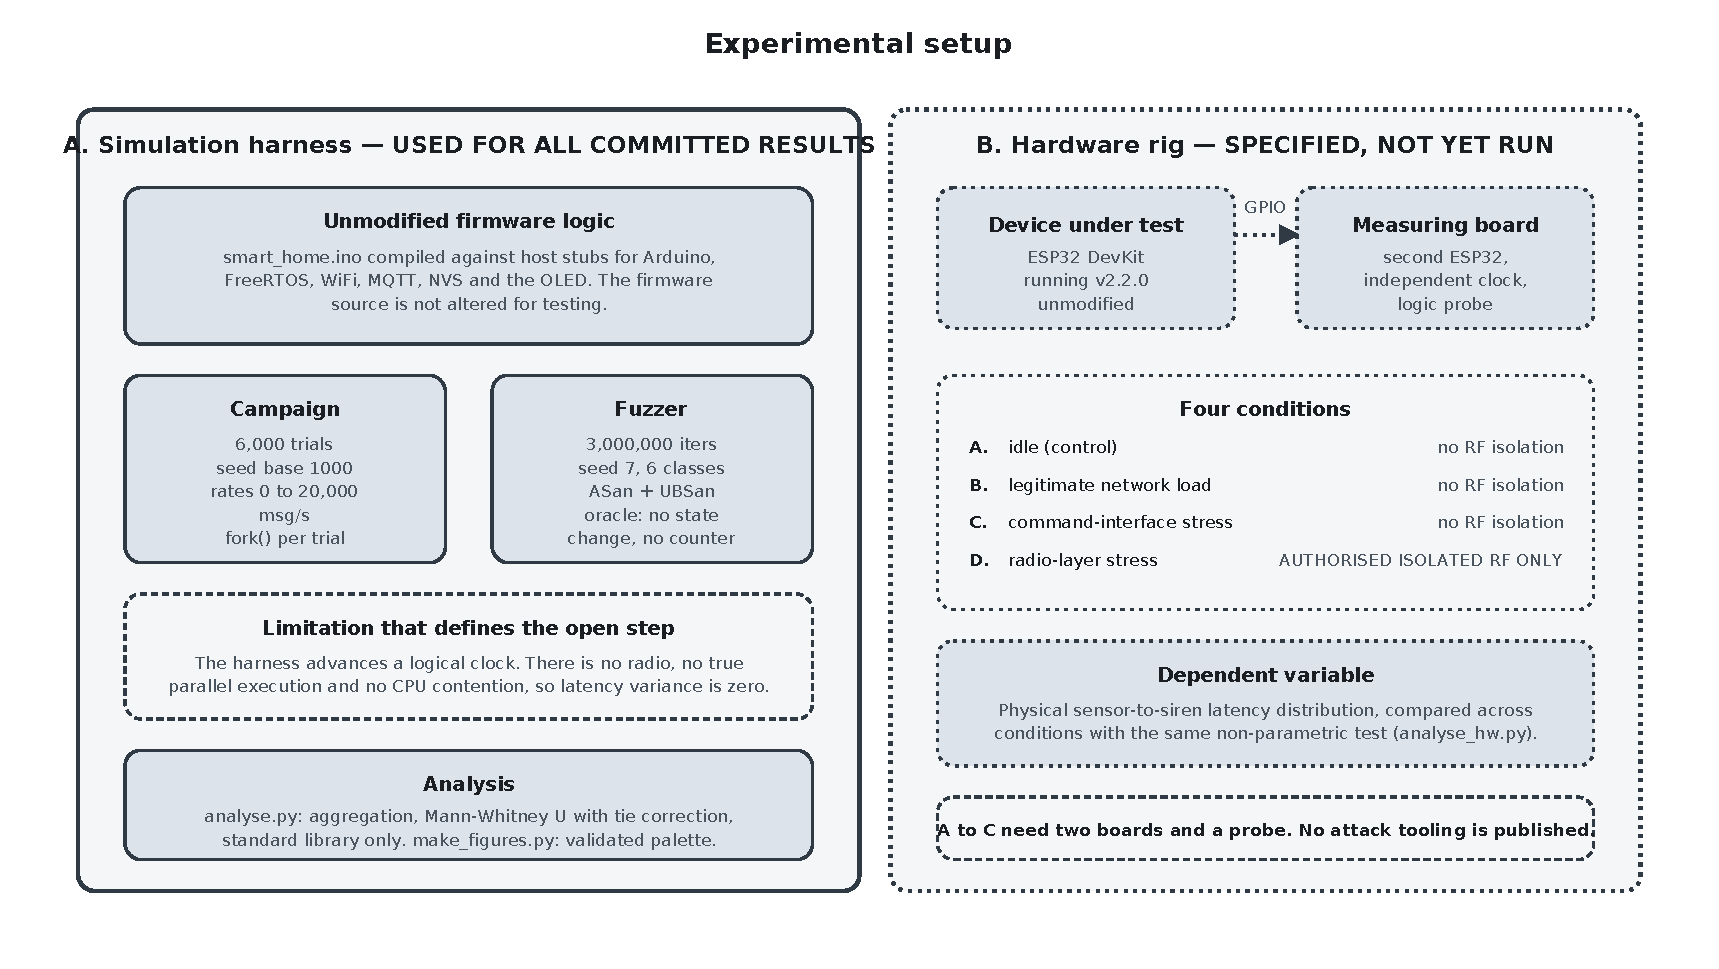
\includegraphics[width=\textwidth]{experimental_setup.pdf}
\caption[Experimental setup]{Experimental setup. Panel~A is everything that has been run: the
host simulation harness (E1--E5) and the real-broker testbed (E6), which is a live Mosquitto
instance and not a simulation. Panel~B is the hardware rig: specified, built as a protocol, and
\textbf{not run}. No number anywhere in this report comes from panel~B.}
\label{fig:setup}
\end{figure}

\section{Defects found in the measurement infrastructure}\label{sec:method-defects}

Four defects were found in the harnesses themselves during this work. Two of them produced
results that flattered the intended conclusion, which is precisely why they are reported here
rather than quietly corrected. A reader assessing the credibility of
Chapter~\ref{ch:results}'s numbers is entitled to know how the instrument was tested.

\begin{enumerate}[leftmargin=1.8em,itemsep=6pt]
  \item \textbf{Operator availability was unattributable.} The original measurement recorded
        whether a legitimate command took effect, but the adversary in the harness could also
        publish \code{ARM} — so an observed state change could not be attributed to the
        operator. Fixed by suppressing adversary \code{ARM} publications for the whole
        measurement prologue.
  \item \textbf{The first fix was itself wrong.} The quiet settling period introduced by that
        fix allowed the token bucket to refill before the measurement, so the rate limiter
        appeared more available than it is. Fixed by holding the suppression across the entire
        prologue rather than part of it.
  \item \textbf{A single-attempt measurement measured the wrong thing.} Availability recorded as
        one boolean per trial was in fact measuring the token bucket's \emph{phase} at the
        instant of the attempt, producing residues of 0.5, 0.9 and 0.995 rather than a rate.
        Fixed by measuring five attempts per trial at 200\,ms intervals, which is why the
        availability denominator is 1,250 and not 300.
  \item \textbf{A button hold shorter than the debounce window.} The harness held the simulated
        button for 40\,ms against a 40\,ms debounce threshold, so local arming was intermittent
        for reasons unrelated to the experiment. Fixed to 80\,ms.
\end{enumerate}

The campaign was re-run from scratch after these corrections, and every number in
Chapter~\ref{ch:results} comes from the corrected harness.

A fifth defect, in the corpus rule rather than the harness, is reported in
Section~\ref{sec:res-corpus}: the rule initially returned zero against this project's own
pre-repair guard, because the identifier it looked for appears there \emph{negated}. Until that
was found, the zero result was meaningless. The eight controls exist as a direct consequence.

\chapter{Results and Statistical Analysis}\label{ch:results}

Every number in this chapter was recomputed from the raw per-trial records during the
preparation of this report, not copied from an earlier document. The recomputation script is
\code{experiments/validate\_figures.py}, which reads \code{ablation.jsonl} rather than the
derived summary.

\section{Statistical treatment}

Three decisions govern every test reported below.

\textbf{Interval estimates.} Proportions are reported with 95\% Wilson score intervals rather
than the normal approximation, because several arms sit at or near $p=0$ or $p=1$ where the
normal interval is degenerate and can extend outside $[0,1]$. Intervals are clamped at the unit
bounds.

\textbf{Hypothesis tests: the design is matched pairs.} Every arm runs on the same 300 seeds with
the same seed-to-attack-rate mapping, so each seed yields a matched pair and only discordant pairs
carry information. The primary test is the exact one-sided McNemar test. An earlier version of
this report used Fisher's exact test, which assumes two independent samples --- an assumption this
design does not satisfy, and which overstated the evidence by roughly fifty orders of magnitude in
one comparison. Fisher figures are retained only as a labelled sensitivity analysis. $\chi^2$ is
avoided because several tables contain zero cells.

\textbf{Clustered observations.} The availability metric takes five operator attempts per trial,
and those five share that trial's token-bucket phase: 231 of 250 rate-limiter trials admitted
either all five or none. The intra-cluster correlation is 0.669, a design effect of 3.68, so 1,250
attempts carry the information of about 340 independent ones. The attempt-level proportion is
reported because it is what an operator experiences; the test is at the trial level, which is the
independent unit.

\textbf{Where no test is reported.} No hypothesis test is applied to a quantity whose variance
is identically zero by construction. The simulation harness advances a logical clock, so the
safety latency is the same constant — 151\,ms, being the sensor confirmation window plus the
loop period — in every trial. A test on two constant-valued samples is trivially satisfied and
carries no information. The pre-registered test for the hardware measurement is in
Appendix~\ref{app:hardware} and was committed before any data existed.

Because every arm is a fixed, pre-declared configuration rather than a selected subset, no
multiplicity correction is applied. This is noted so a reader can judge it rather than infer it.

\section{Trial accounting}

\begin{longtable}{@{}p{0.07\textwidth}p{0.34\textwidth}p{0.20\textwidth}p{0.29\textwidth}@{}}
\toprule
\textbf{ID} & \textbf{Experiment} & \textbf{Scale} & \textbf{Artefact} \\
\midrule
\endhead
E1 & Campaign, baseline build        & 3{,}000 trials        & \code{summary.json} \\
E2 & Campaign, hardened build        & 3{,}000 trials        & \code{summary.json} \\
E3 & Command-path ablation           & 3{,}600 trials        & \code{ablation.jsonl} \\
E4 & Host-build fuzzing              & 3{,}000{,}000 iter.   & \code{fuzz.json} \\
E5 & Detector sensitivity            & 180 grid cells        & \code{sensitivity.jsonl} \\
E6 & Live-broker access control      & 8 scenarios           & \code{broker\_acl.jsonl} \\
E7 & Open-source corpus              & 135 projects          & \code{corpus.json} \\
E8 & Trace conformance               & 19{,}529 transitions  & \code{test\_conformance.py} \\
E9 & Model checking                  & 25 and 660 states     & \code{formal/} \\
\midrule
\multicolumn{2}{@{}l}{\textbf{Total adversarial trials}} & \textbf{9{,}600} &
3{,}000 + 3{,}000 + 3{,}600 \\
\bottomrule
\end{longtable}

\section{E1 and E2: the adversarial campaign}

Across 6,000 trials \textbf{no adversary disarmed the device and no safety invariant was
violated.}

Without command authentication the adversary changed the system state in all 2,500 flooded
trials; with authentication, in none. The availability result is the more informative of the
two: with authentication a legitimate command took effect in all 3,000 trials regardless of
attack rate, while in the baseline, flooding starved it in every flooded trial.

\textbf{What this does not show.} It shows nothing about timing. The safety latency is a
constant in this environment, so the campaign establishes that the \emph{logic} holds under
adversarial load and nothing about whether the \emph{silicon} does.

\section{E3: the command-path ablation}\label{sec:res-ablation}

\subsection{The six command-path designs}

Figure~\ref{fig:ablation} shows three properties across the six designs.

\begin{figure}[htbp]
\centering
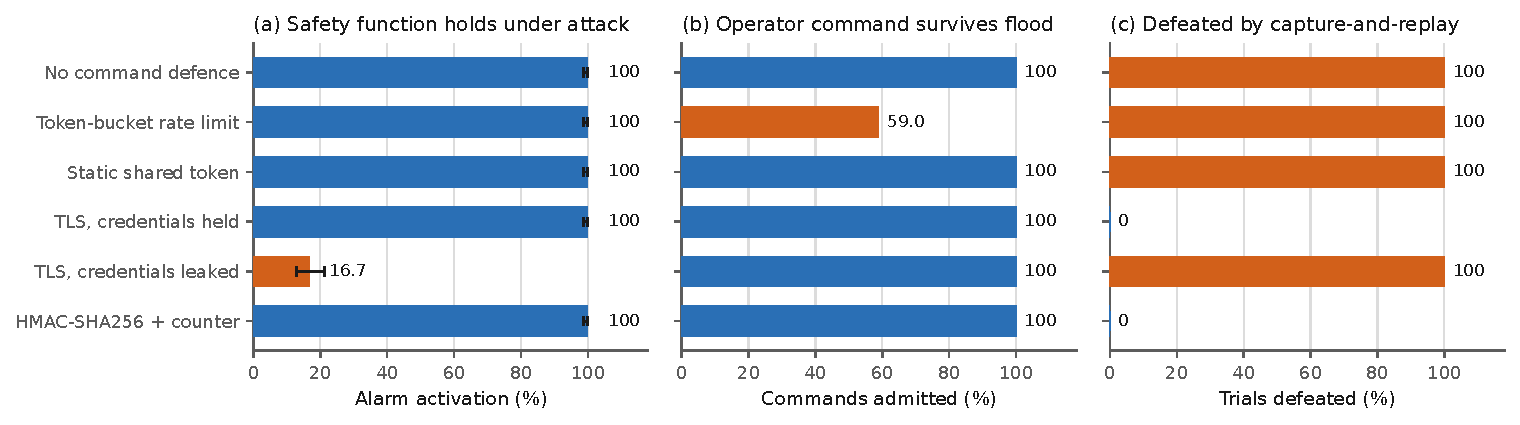
\includegraphics[width=\textwidth]{ablation_results.pdf}
\caption[Command-path ablation results]{Command-path ablation. 300 trials per bar in panels (a)
and (c); 1,250 operator attempts per bar in panel (b). Whiskers in (a) are 95\% Wilson score
intervals. Panel (c) inverts the reading: there a high value is the failure, so the colour rule
inverts with it, and blue continues to mean ``this design holds the property''.}
\label{fig:ablation}
\end{figure}

\begin{longtable}{@{}p{0.27\textwidth}rrrr@{}}
\toprule
\textbf{Design} & \textbf{Alarm} & \textbf{95\% Wilson} & \textbf{Avail.} & \textbf{Replay} \\
\midrule
\endhead
No command defence        & 300/300 & [98.7, 100.0] & 100.0\% & 100\% \\
Token-bucket rate limit   & 300/300 & [98.7, 100.0] & \textbf{59.0\%} & 100\% \\
Static shared token       & 300/300 & [98.7, 100.0] & 100.0\% & 100\% \\
TLS, credentials held     & 300/300 & [98.7, 100.0] & 100.0\% & 0\% \\
TLS, credentials leaked   & \textbf{50/300} & \textbf{[12.9, 21.3]} & 100.0\% & 100\% \\
HMAC-SHA256 + counter     & 300/300 & [98.7, 100.0] & 100.0\% & 0\% \\
\bottomrule
\end{longtable}

\subsection{Three findings}

\textbf{The three properties fail independently.} This is the central result of the ablation and
it is not what one would assume. The rate limiter preserves the safety function and replay
resistance is unchanged at 100\% defeated, yet it costs \textbf{41\% of legitimate operator
commands}. The static token does the reverse: every operator command is admitted and replay
resistance is nil. Only the counter-bound message authentication code holds all three. A designer who treats
``security'' as one property will choose badly here.

Paired by seed at the trial level, 112 pairs are discordant and all favour the authenticated
design: McNemar exact, one-sided, $p = 1.9 \times 10^{-34}$. (Fisher, ignoring both the pairing
and the clustering, would give $3.5 \times 10^{-184}$.)

The aggregate is also the wrong summary of the limiter's own behaviour, and the per-rate figures
are what a reader needs: 82 of 250 operator attempts admitted at 10\,commands/s, \textbf{0 of 250
at 100\,commands/s}, 155 of 250 at 1,000, and all 250 at both 5,000 and 20,000. The cost is not
monotonic in attack intensity and the extremes are the benign cases, because an arrival finding
the bucket below the admission threshold is rejected \emph{without consuming a token}: an extreme
flood pins the bucket just under the threshold and leaves enough refill for the next legitimate
arrival. A defender who tunes the limiter against the worst flood they can generate measures no
availability cost at all, and meets the complete lockout in the field two orders of magnitude
lower.

\textbf{Transport security alone is contingent on credential secrecy.} With credentials held,
TLS gives 100\% alarm activation and no replay. With a single credential leaked, alarm
activation falls to 16.7\%, 95\% Wilson [12.9, 21.3], and the adversary disarms the device in
246 of 300 trials. Of the 300 matched pairs, 250 are discordant and every one lost the alarm when
the credential leaked, with none gaining it: McNemar exact, one-sided,
$p = 5.5 \times 10^{-76}$. (Fisher would give $9.8 \times 10^{-119}$.)

\textbf{The alarm still firing is not the same as the system being secure.} In the
\code{none}, \code{ratelimit} and \code{token} arms the alarm fires in all 300 trials, and all
three are completely defeated by capture-and-replay. Panel (a) read alone would suggest that no
command defence is as safe as a message authentication code. Panel (c) is what prevents that
reading, and this is why the figure has three panels rather than one.

\section{Broker authorisation against message authentication}\label{sec:res-credential}

\subsection{The nine-cell matrix}

Figure~\ref{fig:credential} indexes outcomes by \emph{which secret the adversary holds} rather
than by mechanism, because that is the comparison the design question requires.

\begin{figure}[htbp]
\centering
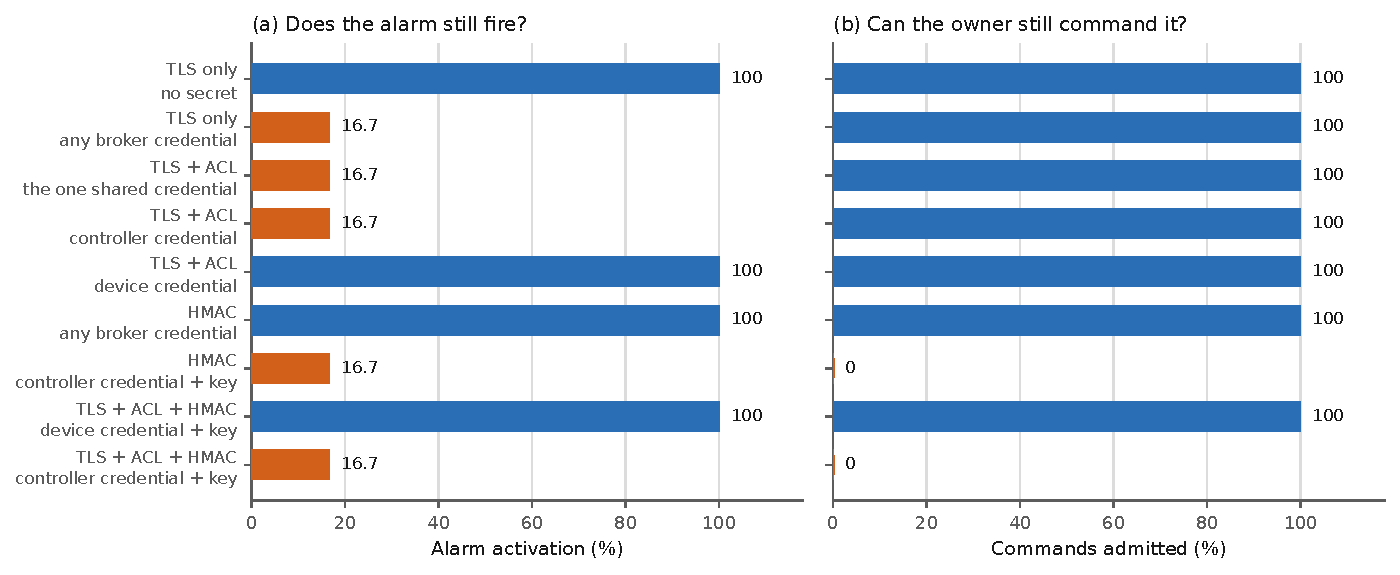
\includegraphics[width=\textwidth]{credential_matrix.pdf}
\caption[Security compromise comparison]{Alarm activation and operator availability for nine
combinations of control and compromised secret. The bottom row is the layered build under a
compromised controller host: it fails, and is drawn at the same weight as every other row.}
\label{fig:credential}
\end{figure}

\begin{longtable}{@{}p{0.19\textwidth}p{0.26\textwidth}rrr@{}}
\toprule
\textbf{Control} & \textbf{Compromise} & \textbf{Alarm} & \textbf{Operator admitted} &
\textbf{Disarms} \\
\midrule
\endhead
TLS only        & none                       & 300/300 & 1250/1250 & 0 \\
TLS only        & any broker credential      & 50/300  & 1250/1250 & 246 \\
TLS + ACL       & the one shared credential  & 50/300  & 1250/1250 & 246 \\
TLS + ACL       & controller credential      & 50/300  & 1250/1250 & 246 \\
TLS + ACL       & device credential          & 300/300 & 1250/1250 & 0 \\
HMAC + counter  & any broker credential      & 300/300 & 1250/1250 & 0 \\
HMAC + counter  & controller cred.\ + key    & 50/300  & \textbf{0/1250} & 234 \\
TLS+ACL+HMAC    & device cred.\ + key        & 300/300 & 1250/1250 & 0 \\
TLS+ACL+HMAC    & controller cred.\ + key    & 50/300  & \textbf{0/1250} & 234 \\
\bottomrule
\end{longtable}

\subsection{Neither control dominates}

The matrix shows that broker authorisation and application-layer authentication fail under
\emph{different} compromises, and that neither contains the other.

The access control list contains a compromised \emph{device} credential, which the message
authentication code does not — because the command key lives in the same flash image as the
device's broker credential, so a flash dump yields both. Conversely the message authentication
code contains a compromised \emph{controller} credential, which the access control list cannot
— because the list must permit that identity to publish commands.

\subsection{An unanticipated negative result: owner lockout}

Two rows show \textbf{0 of 1,250} operator commands admitted. This was not predicted.

Under key compromise the adversary signs commands with a counter far above the operator's. The
device persists that counter, as it must in order to resist replay. Every subsequent legitimate
command then carries a lower counter and is correctly rejected as a replay. The mechanism that
defeats capture-and-replay has become a lockout against the legitimate owner.

\textbf{The mechanism is not new; the measurement is.} A literature check carried out for this
report found the mechanism stated as background in work on ZigBee replay attacks: Wara and
Yu~\cite{wara2020} note that an attacker can set a device's frame counter above its normal value
so that subsequent lower-counter frames are discarded. They state it in passing, without a
citation and without an experiment, and their own measurements go the other way --- they test
whether raising a captured frame's counter lets a \emph{replay} succeed, not whether it blocks
legitimate traffic.

What this work adds is therefore not the observation but the quantification and the attribution:
the lockout is complete rather than partial (0 of 1,250), it arises from a design decision made
for a defensible reason, and it shows that replay resistance and owner availability are coupled
under key compromise rather than independent. An earlier draft of this report claimed the
mechanism had not been reported at all. That claim was wrong and has been withdrawn.

\subsection{An overclaim found by measuring the missing arm}\label{sec:res-overclaim}

An earlier draft of this work stated that the layered configuration ``survives every case''.
That statement was false, and it was found to be false by running the arm the draft had not run.

The layered configuration survives every single-secret compromise \emph{and} a device flash
dump. It falls to a compromised controller host. Since the flash dump requires physical access
and the controller-host compromise does not, the configuration survives the expensive scenario
and fails the cheap one. Figure~\ref{fig:security} draws both.

\begin{figure}[htbp]
\centering
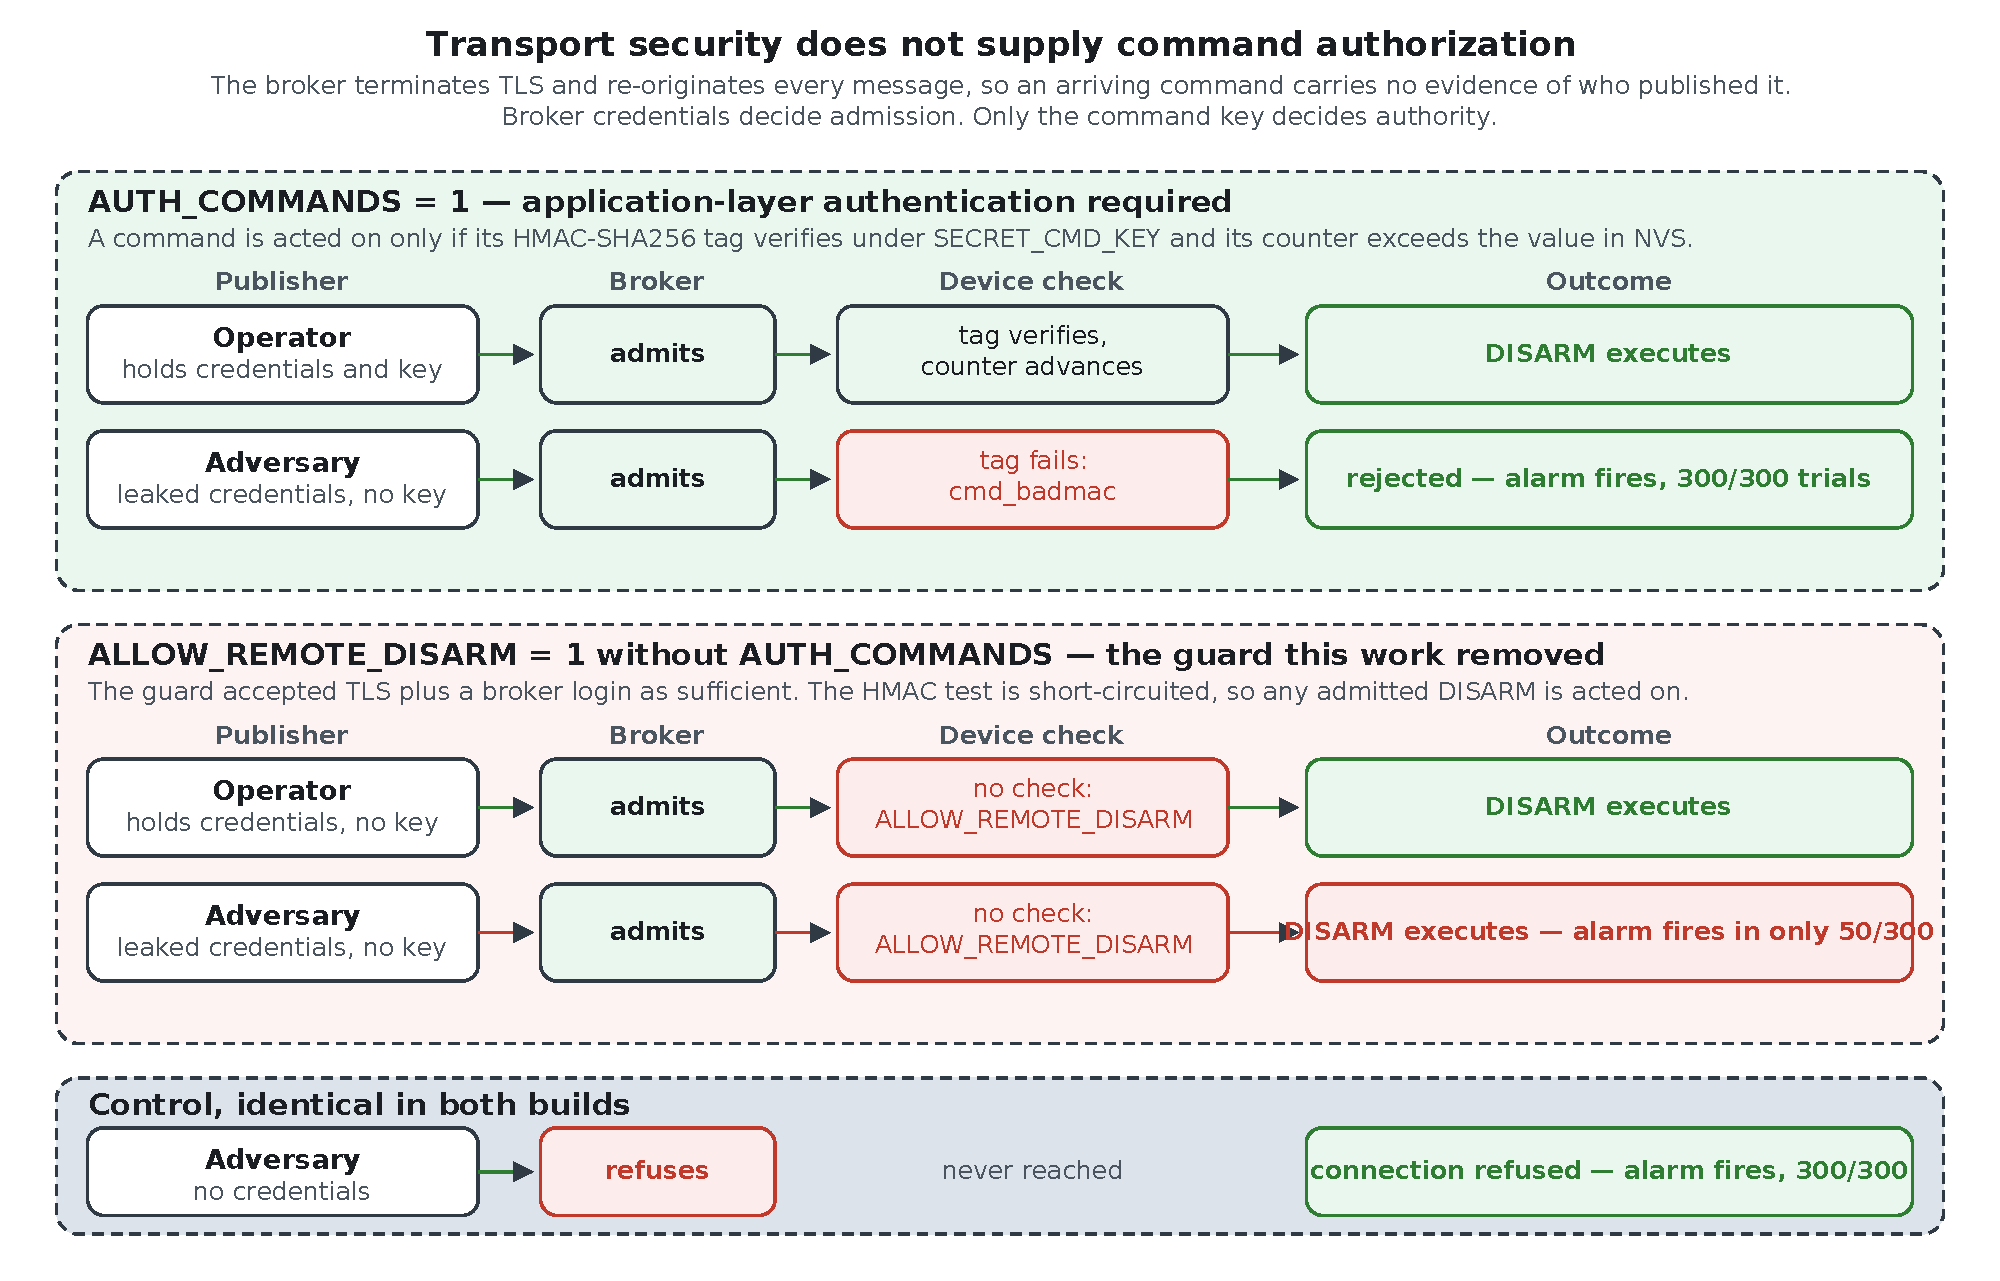
\includegraphics[width=\textwidth,height=0.74\textheight,keepaspectratio]{security_paths.pdf}
\caption[Transport security versus command authorisation]{Where broker credentials decide
admission and where the command key decides authority. The third row of the upper panel is the
compromised controller host, holding both a permitted credential and the key: neither layer
refuses it, and the alarm fires in only 50 of 300 trials.}
\label{fig:security}
\end{figure}

\section{E6: results against a live broker}\label{sec:res-broker}

All eight scenarios were run against Mosquitto 2.0.18 over TLS 1.2 with a private certificate
authority. The verdicts reproduce: re-running the experiment on a freshly installed broker in a
clean environment during the preparation of this report returned verdicts identical to the
committed run, with only the broker's own log timestamps and random client identifiers
differing.

\begin{longtable}{@{}llccc@{}}
\toprule
& \textbf{Adversary identity} & \textbf{Connected} & \textbf{Delivered} &
\textbf{Would execute} \\
\midrule
\endhead
\multicolumn{5}{@{}l}{\textit{Per-client access control list}} \\
control & controller (legitimate)      & yes & yes & yes \\
A       & no credentials               & \textbf{no} & no  & no \\
C       & controller credential        & yes & yes & \textbf{yes} \\
D       & device credential            & yes & \textbf{no}  & no \\
E       & device credential + key      & yes & \textbf{no}  & no \\
E$'$    & controller credential + key  & yes & yes & \textbf{yes} \\
\midrule
\multicolumn{5}{@{}l}{\textit{Single shared credential}} \\
control & controller, shared ACL       & yes & yes & yes \\
B       & shared credential            & yes & yes & \textbf{yes} \\
\bottomrule
\end{longtable}

\textbf{E and E$'$ are the decisive pair.} The \emph{same valid signature}, carried by the
device identity, is not delivered; carried by the controller identity, it is. What stops
scenario E is therefore the access control list and not the signature. This is the result that
could not be established by modelling alone, and it is the reason the experiment was worth
running against real broker software.

\section{E5: detector parameter sensitivity}

The sweep produced a correction rather than a confirmation. At the detector's original shipped
configuration — threshold 8 frames within a 2,000\,ms window — the detector fired in
\textbf{1,597 of 2,000} benign ten-minute runs (79.85\%). That is not a detector; it is an
alarm that reports almost continuously under normal conditions.

The firmware now ships \code{DEAUTH\_THRESHOLD = 12}. The sweep is reported because the
original value was wrong by a wide margin and the sweep is what revealed it.

\section{E4: fuzzing}

3,000,000 iterations across six input classes under both sanitizers produced \textbf{no crash,
no sanitizer report and no accepted input}: no input changed state or advanced the counter
without a valid tag.

\textbf{What this is evidence of, and what it is not.} It is evidence of memory safety and
parser robustness. It is \emph{not} independent evidence of authentication soundness: against a
128-bit tag, zero forgeries in three million attempts is the expected outcome whether the
implementation is sound or not, since the probability of a chance forgery is $2^{-128}$.

\section{E7: the corpus study, and a negative result}\label{sec:res-corpus}

\subsection{Rule 1 found nothing}

The precise guard rule returned \textbf{zero hits across 135 projects}.

That is reported as a zero. \textbf{No claim is made that the pattern is widespread}, and the
finding remains a single-system case study.

The zero is also explained rather than left bare. Only 30 of the 135 projects both subscribe to
MQTT and contain any application-authentication identifier at all, and reading those shows that
most matches sit in vendored third-party code rather than in the project's own command path.
The corpus is biased by construction — 22 fixed queries, a minimum of 3 stars, a size cap of
80\,MB, archived repositories and forks excluded — and those criteria are recorded with the
rejection counts in \code{corpus.json}.

\subsection{The rule was wrong at first}

This matters for the credibility of the zero. The rule initially returned zero against
\emph{this project's own pre-repair guard}, because it treated any mention of the
authentication identifier as evidence that authentication was required — and in the defective
guard that identifier appears \emph{negated}. Until this was found, the zero result was
meaningless.

Eight controls now exist as a direct consequence, including the project's own pre-repair guard
as a positive control and its repaired guard as a negative control. All eight pass.

\subsection{Rule 2 and the nine confirmed projects}

The looser heuristic flagged 18 of 135. Reading all 18 by hand gave 9 confirmed and 9 false
positives.

This is reported as an \textbf{existence claim and not a rate}. The rule over-counts monitoring
projects by roughly half and under-counts non-GPIO actuation by an unknown amount: three of the
nine confirmed cases actuate through Modbus, RF or serial frames and were caught only by an
incidental GPIO write. The 18/135 figure is therefore not a prevalence estimate and must not be
read as one.

\section{E8 and E9: conformance and model checking}

\textbf{Trace conformance.} 19,529 firmware transitions across three ablation modes — 7,044,
5,282 and 7,206 — checked against the transition relation parsed from \code{AlarmFSM.tla}.
\textbf{Zero disallowed transitions.} The negative control confirms that a forbidden
\code{Disarmed} $\rightarrow$ \code{Alarm} transition \emph{is} rejected, which is what makes
the 19,529 meaningful: a checker that accepts everything would also report zero violations.

\textbf{Model checking.} \code{AlarmFSM}: 166 states generated, 25 distinct.
\code{Isolation}: 2,686 generated, 660 distinct. Both exhaustive. The third configuration and
its purpose are the subject of Chapter~\ref{ch:formal}.

\section{Summary of statistical values}

Every value below was recomputed from the raw records during the preparation of this report.

\begin{longtable}{@{}p{0.47\textwidth}p{0.22\textwidth}p{0.21\textwidth}@{}}
\toprule
\textbf{Claim} & \textbf{Recomputed} & \textbf{Status} \\
\midrule
\endhead
Leaked-credential alarm activation 16.7\%        & 50/300 = 16.67\%        & exact \\
95\% Wilson interval [12.9\%, 21.3\%]            & [12.9, 21.3]            & exact \\
Rate limiter admits 59.0\% of operator commands  & 737/1250 = 59.0\%       & exact \\
McNemar exact (paired), availability             & $1.93\times10^{-34}$    & exact, primary \\
McNemar exact (paired), transport arms           & $5.53\times10^{-76}$    & exact, primary \\
Intra-cluster correlation, 5 attempts per trial  & 0.669 (design eff.\ 3.68) & exact \\
Fisher exact, unpaired sensitivity only          & $3.53\times10^{-184}$, $9.83\times10^{-119}$ & superseded \\
Adversary disarms in 246 of 300 trials           & 246                     & exact \\
Owner lockout 0 of 1,250                         & 0/1250                  & exact \\
Detector default fired in 1597/2000 benign runs   & 1597/2000 = 79.85\%     & exact \\
TLC distinct states, 25 and 660                  & 25 and 660              & exact \\
Trace transitions, 19,529                        & 7044+5282+7206          & exact \\
\bottomrule
\end{longtable}

\chapter{Formal Verification}\label{ch:formal}

Two TLA+ specifications were written for this project and are checked exhaustively by TLC on
every push. This chapter states what they establish, and — with equal emphasis — what they do
not, because the second specification is named \code{Isolation} and that name invites a stronger
reading than the model supports.

The chapter also records a defect in the first specification. For part of this project the
specification passed every check while being incapable of failing. That is reported here rather
than quietly repaired, because it is the most instructive methodological result in the work.

\section{Why formal methods were applied at all}

The firmware's safety claim is universal: \emph{no} sequence of adversarial messages causes an
unauthorised disarm. Testing cannot establish a universal claim over an unbounded input space;
it can only fail to refute it. The adversarial campaign of Chapter~\ref{ch:results} ran 9,600
trials and found no violation, which is evidence but not proof. Exhaustive model checking over
a bounded abstraction is the complementary instrument: it enumerates every reachable state of
the abstraction and therefore \emph{proves} the invariant within that abstraction's bounds.

The two instruments fail in different directions, which is why both are used. The model may
abstract away the very detail that breaks in reality; the experiment covers reality but only
the paths it happened to take.

\section{Specification 1: the alarm state machine}

\subsection{What is modelled}

\code{formal/AlarmFSM.tla} models the five-state arm/disarm machine and the authenticated
command path, over three variables:

\begin{itemize}[leftmargin=1.6em,itemsep=3pt]
  \item \code{state} --- one of \code{Disarmed}, \code{ExitDelay}, \code{Armed},
        \code{EntryDelay}, \code{Alarm}
  \item \code{ctr} --- the highest accepted authenticated command counter
  \item \code{badDisarm} --- set \code{TRUE} if an unauthenticated remote disarm ever takes
        effect
\end{itemize}

\textbf{Time is abstract.} A delay expires as a nondeterministic step rather than by counting
milliseconds. This is the correct level of abstraction for reasoning about \emph{which
transitions are reachable and who may cause them}, and it is the wrong level for reasoning about
\emph{how long} anything takes. No timing conclusion is drawn from this model anywhere in this
report.

\subsection{Properties checked}

\begin{longtable}{@{}p{0.27\textwidth}p{0.11\textwidth}p{0.50\textwidth}@{}}
\toprule
\textbf{Property} & \textbf{Kind} & \textbf{Statement} \\
\midrule
\endhead
\code{TypeOK}              & invariant & All three variables stay in their declared domains \\
\code{NoUnauthRemoteDisarm}& invariant & \code{badDisarm = FALSE}: the system never leaves an
armed state because of an unauthenticated remote command \\
\code{NoAlarmWhenDisarmed} & invariant & The siren is never on while disarmed \\
\code{CounterMonotonic}    & temporal  & $[][ctr' \geq ctr]$: the replay counter never
decreases \\
\code{EntryLeadsToResolve} & liveness  & An entry delay always ends in \code{Alarm} or
\code{Disarmed}; the system cannot get stuck mid-entry \\
\code{AlarmReArms}         & liveness  & The alarm always ends, in re-arm or disarm \\
\bottomrule
\end{longtable}

The liveness properties require fairness on the three timed transitions
(\code{ExitExpire}, \code{EntryExpire}, \code{AlarmExpire}), supplied by weak fairness in
\code{Spec}. No fairness is assumed for any adversary action.

\subsection{Result}

With \code{MaxCtr = 4} and \code{AllowUnauthDisarm = FALSE}: \textbf{166 states generated, 25
distinct, 0 left on queue, no error found.} The run is exhaustive over the bounded state space,
and both temporal branches were checked over the complete space.

\section{The vacuity defect, and the repair}\label{sec:formal-vacuity}

\subsection{What was wrong}

In the original specification the unauthenticated-command action was written as an
unconditional refusal:

\begin{lstlisting}[style=tla,caption={The defective action, as originally written (reconstructed
from the repair commit).},label={lst:vacuous}]
\* An UNauthenticated remote command is refused, exactly as the firmware does.
RemoteUnauthDisarm ==
  /\ state \in ArmedLike
  /\ UNCHANGED <<state, ctr, badDisarm>>
\end{lstlisting}

The comment asserts the conclusion. \code{badDisarm} was initialised \code{FALSE} and left
\code{UNCHANGED} by \emph{every} action in the specification, so no reachable behaviour could set
it. The invariant \code{NoUnauthRemoteDisarm} was therefore \textbf{unfalsifiable by
construction}: not proved, but incapable of failing.

TLC reported success. The success meant nothing.

\subsection{Why this mattered more than an ordinary bug}

The firmware contained a real defect of exactly the kind this invariant was written to catch: a
compile-time guard that admitted remote disarm without application-layer authentication. The
ablation experiment found it. The model checker, which existed specifically to find it, could
not have found it under any circumstances.

The specification had embedded the same unverified assumption that the firmware got wrong. A
passing formal check had been taken as evidence for a property that the check was structurally
unable to test. This is the project's central methodological finding, generalised in
Chapter~\ref{ch:conclusion}.

\subsection{The repair}

The build switch is now a model parameter rather than a hard-coded refusal:

\begin{lstlisting}[style=tla,caption={The repaired action: the configuration is a parameter, so
the violating behaviour exists and is reachable under one valuation.},label={lst:repaired}]
RemoteUnauthDisarm ==
  /\ state \in ArmedLike
  /\ IF AllowUnauthDisarm
       THEN /\ state' = "Disarmed"
            /\ badDisarm' = TRUE
            /\ UNCHANGED ctr
       ELSE UNCHANGED <<state, ctr, badDisarm>>
\end{lstlisting}

\subsection{The third configuration: a check that must fail}

The repair alone is not sufficient, because a future edit could reintroduce the vacuity and the
suite would again report success. A third configuration therefore exists whose \emph{required
outcome is a violation}.

\code{AlarmFSM\_unsafe.cfg} sets \code{AllowUnauthDisarm = TRUE}, modelling the
\code{ALLOW\_REMOTE\_DISARM} build with no application-layer authentication.
\code{formal/run\_tlc.sh} inverts the exit condition for this run and additionally requires the
specific string \code{Invariant NoUnauthRemoteDisarm is violated} in TLC's output:

\begin{lstlisting}[style=sh,caption={The inverted check. A \emph{passing} TLC run is treated as a
build failure.},label={lst:invertedcheck}]
if java -cp "$JAR" tlc2.TLC -config AlarmFSM_unsafe.cfg AlarmFSM.tla > /tmp/tlc_unsafe.out 2>&1
then
  echo "FAIL AlarmFSM_unsafe: TLC found no violation, so the invariant is vacuous again"
  fail=1
elif grep -q "Invariant NoUnauthRemoteDisarm is violated" /tmp/tlc_unsafe.out; then
  echo "PASS AlarmFSM_unsafe: TLC reports the expected NoUnauthRemoteDisarm violation"
\end{lstlisting}

Requiring the specific invariant name, rather than merely a non-zero exit, matters: a syntax
error, a missing constant or a parse failure also produce a non-zero exit, and would otherwise be
silently accepted as the expected violation.

TLC reports the expected violation on every run. The invariant is now known to be falsifiable,
which is what licenses reading its success in the safe configuration as evidence.

\section{Specification 2: the isolation model}\label{sec:formal-isolation}

\subsection{What is modelled}

\code{formal/Isolation.tla} models the two-task structure over seven variables:
\code{safetySteps}, \code{produced}, \code{queued}, \code{delivered}, \code{dropped},
\code{netState} and \code{netOwnsState}.

The network task is modelled \textbf{adversarially and with no fairness whatsoever}. It may move
between \code{idle}, \code{busy}, \code{stalled} and \code{down}; it may stall for an unbounded
time, as in a slow DNS, TCP or TLS call; it may fail to publish; and it may crash and restart.
Only the safety task is given weak fairness. The question the model answers is whether the
safety task still progresses when the network task is permitted to behave as badly as it likes
forever.

\subsection{Properties checked}

\begin{longtable}{@{}p{0.26\textwidth}p{0.11\textwidth}p{0.51\textwidth}@{}}
\toprule
\textbf{Property} & \textbf{Kind} & \textbf{Statement} \\
\midrule
\endhead
\code{TypeOK}               & invariant & All seven variables stay in their domains \\
\code{SafetyCanAlwaysStep}  & invariant &
$(\mathit{safetySteps} < \mathit{MaxEvents}) \Rightarrow \mathrm{ENABLED}\ \mathit{SafetyStep}$
--- in every reachable state the safety task is enabled \\
\code{NoNetworkWrite}       & invariant & \code{netOwnsState = FALSE}: the network task never
writes the alarm state \\
\code{QueueBounded}         & invariant & $\mathit{queued} \leq \mathit{QCap}$: the writer drops
instead of blocking \\
\code{NoSilentLoss}         & invariant &
$\mathit{produced} = \mathit{delivered} + \mathit{queued} + \mathit{dropped}$ \\
\code{SafetyProgress}       & liveness  &
$\Diamond(\mathit{safetySteps} = \mathit{MaxEvents})$: the safety task is never starved \\
\bottomrule
\end{longtable}

\code{SafetyCanAlwaysStep} is the architectural claim stated formally. Its force comes from what
the guard of \code{SafetyStep} mentions: \code{safetySteps} and \code{produced} only, and nothing
owned by the network side. Because the enabling condition is independent of \code{netState}, no
network behaviour can disable it. \code{NoSilentLoss} is the drop-oldest policy stated as an
accounting identity: an event is delivered, still queued, or counted as dropped, and never
disappears.

\subsection{Result}

With \code{QCap = 16} and \code{MaxEvents = 8}: \textbf{2,686 states generated, 660 distinct, 0
left on queue, no error found}, with the temporal property checked over the complete 660-state
space.

\subsection{What this model does and does not establish}

This distinction is the most important sentence in the chapter, and it is maintained verbatim
throughout this report and the manuscript.

\textbf{What it establishes.} \emph{Logical} isolation. The safety task's enabling condition is
independent of every network-side variable, so there exists no reachable state --- under
unbounded stalling, flooding, publication failure or crash --- in which the network side has
disabled the safety side. In the firmware this corresponds to the asymmetric mutex timeout: the
safety loop calls \code{xSemaphoreTake(statusMutex, 0)}, so its blocking term is identically
zero, by construction and not by measurement.

\textbf{What it does not establish.} \emph{Physical timing invariance.} The model has no notion
of microseconds, cache lines, bus arbitration, interrupt latency, radio duty cycle, or the
thermal and clock behaviour of a real die. Two cores on one package contend for shared silicon
in ways a seven-variable state machine cannot represent. Logical isolation does not imply that
the safety loop's measured wall-clock period is invariant to network load on real hardware, and
nothing in this project has measured whether it is.

The firmware is designed so that the \emph{blocking} component of that period is zero. Whether
the \emph{total} period is invariant is an empirical question about silicon, requiring hardware
conditions A--D. Those were not executed; Appendix~\ref{app:hardware} records why, and the
pre-registered analysis plan that was committed before any data existed.

\section{Trace conformance: connecting the model to the code}

A specification can be correct about a machine the firmware does not implement. Trace
conformance is the bridge.

\code{experiments/test\_conformance.py} parses the transition relation directly from
\code{AlarmFSM.tla} --- rather than re-encoding it in Python, where it could drift --- and checks
every recorded firmware state transition against it.

\textbf{19,529 transitions} across three ablation modes: 7,044, 5,282 and 7,206.
\textbf{Zero disallowed transitions.}

The figure is meaningful only because of the negative control. The same checker is given a
deliberately forbidden transition, \code{Disarmed} $\rightarrow$ \code{Alarm}, and is required to
reject it. It does. Without that control, a checker that accepted everything would also report
zero violations across 19,529 transitions, and the result would be indistinguishable from the
one reported here. This is the same reasoning as the inverted TLC configuration in
Section~\ref{sec:formal-vacuity}, applied to a different instrument.

\section{Summary}

\begin{longtable}{@{}p{0.23\textwidth}p{0.20\textwidth}p{0.45\textwidth}@{}}
\toprule
\textbf{Configuration} & \textbf{Result} & \textbf{Required outcome} \\
\midrule
\endhead
\code{AlarmFSM.cfg}        & 25 distinct states, no error  & pass \\
\code{Isolation.cfg}       & 660 distinct states, no error & pass \\
\code{AlarmFSM\_unsafe.cfg}& \code{NoUnauthRemoteDisarm} violated &
\textbf{violation required}; a pass is a build failure \\
\code{test\_conformance.py}& 19,529 transitions, 0 violations & pass, with the negative control
rejected \\
\bottomrule
\end{longtable}

All four are re-run by continuous integration on every push, so neither the vacuity defect nor a
silently accepting conformance checker can recur without the build failing.

\chapter{Security Evaluation}\label{ch:security}

This chapter evaluates the system against the threat model of Chapter~\ref{ch:req} and
reports two results that the project did not set out to find: that the layered configuration
fails under one specific compromise, and that the mechanism defending against replay can lock out
the legitimate owner. Both are reported as findings about this design rather than as
limitations of the evaluation.

\section{The threat model, restated with outcomes}

Each scenario is defined by \emph{what the adversary holds}, not by what mechanism is deployed.
The access column is material: it separates a scenario requiring physical possession of the
device from one that can be mounted from anywhere on the network.

\begin{longtable}{@{}p{0.05\textwidth}p{0.26\textwidth}p{0.13\textwidth}p{0.42\textwidth}@{}}
\toprule
\textbf{ID} & \textbf{Adversary holds} & \textbf{Access} & \textbf{Outcome against the layered
build} \\
\midrule
\endhead
A & nothing                     & remote   & Refused at the broker; the connection is not
established \\
B & the one shared credential   & remote   & \textbf{Defeats} a shared-credential deployment;
refused by per-client authorisation \\
C & controller broker credential& remote   & Delivered; refused by the message authentication
code \\
D & device broker credential    & remote   & Refused by the access control list; the device
identity may not publish commands \\
E & device credential + command key & \textbf{physical} & \textbf{Survived}: refused by the
access control list despite a valid signature \\
E$'$ & controller credential + command key & \textbf{remote} & \textbf{Defeats the layered
build}: neither layer refuses it \\
\bottomrule
\end{longtable}

\subsection{Why E and E$'$ are the decisive pair}\label{sec:sec-eprime}

Scenarios E and E$'$ carry \emph{the same cryptographically valid signature}. They differ only in
the broker identity that transmits it.

Under E the signature arrives from the device identity. The access control list grants that
identity \code{read} on \code{home/alarm/+/cmd} and \code{write} on \code{home/alarm/+/stat};
it does not grant \code{write} on the command topic. The broker refuses the publication, so the
valid signature never reaches the device.

Under E$'$ the same signature arrives from the controller identity, which must hold
\code{write} on the command topic for the system to function at all. The broker delivers it, and
the message authentication code verifies --- correctly, because the signature is valid. The
command executes.

\textbf{What stops scenario E is therefore the access control list and not the signature.} This
cannot be established by reasoning about the cryptography, and it is the result that justified
running experiment E6 against real broker software rather than modelling broker behaviour. Both
scenarios were executed against Mosquitto 2.0.18 over TLS 1.2 with a private certificate
authority; the verdicts in Section~\ref{sec:res-broker} are the broker's own.

\subsection{An asymmetry in cost}

E requires physical possession of the device and a flash dump. E$'$ requires compromise of the
controller host --- a general-purpose machine, typically a Raspberry Pi or a server, reachable
over the network and administered by software with its own vulnerability history.

The layered configuration therefore \textbf{survives the expensive attack and falls to the cheap
one.} That is the opposite of the ordering a defender would choose, and it is stated plainly
because an earlier draft of this work did not state it.

\section{Flash extraction and what is actually protected}\label{sec:sec-flashdump}

\subsection{The threat}

The ESP32's SPI flash can be read over the serial interface with standard vendor tooling unless
flash encryption and secure boot are enabled. This firmware does not enable them. Anyone with
physical possession of the device can therefore recover the entire image, which contains both the
device's broker credential and \code{SECRET\_CMD\_KEY}.

\subsection{Why the device survives it anyway}

This is a genuine positive result and is worth stating precisely, because it is easy to
overstate.

The device survives a flash dump \emph{not} because the key is protected --- it is not --- but
because \textbf{the identity whose secrets were extracted is not authorised to issue commands.}
The access control list is deny-by-default and grants the device identity publication rights only
on the status topic. An adversary holding everything in the device's flash can sign a
valid \code{DISARM} command and still cannot get it accepted, because the broker refuses to
carry it.

This is a defence-in-depth result in the strict sense: a complete failure of secret
confidentiality at one layer is contained by authorisation at another.

\subsection{What it does not mean}

It does not mean key extraction is harmless. It means key extraction \emph{from the device} is
contained. Key extraction from the controller host is scenario E$'$, which is not contained. The
protection comes from \emph{which} identity holds the key, not from the key being hard to obtain.

Three consequences follow and are recorded in Chapter~\ref{ch:limitations}: a deployment that
issues one credential to both parties collapses E$'$ and E into the same scenario and loses the
protection entirely; a deployment whose access control list grants the device identity write
access on the command topic, for convenience during commissioning, loses it as well; and flash
encryption with secure boot would address the extraction itself rather than only containing it.

\section{The compile-time guard}\label{sec:sec-guard}

\subsection{The original defect}

The firmware originally admitted remote disarm when the build had transport security and a
broker login, on the reasoning that a client which has authenticated to the broker over TLS is
trustworthy. That reasoning is wrong for a specific and documented reason: in MQTT 3.1.1 the
broker \emph{re-originates} messages. The subscriber receives a message from the broker, not from
the publisher, and the protocol carries no publisher identity to the subscriber. Transport
authentication tells the broker who connected; it tells the device nothing about who authored a
command.

Broker credentials are bearer tokens. One leaked credential makes the adversary a legitimate
client, and the ablation measured the consequence: alarm activation falls from 300/300 to 50/300,
with the adversary disarming the device in 246 of 300 trials
(Section~\ref{sec:res-ablation}).

\subsection{The repair, and why it is a build-time error}

The defective configuration is now rejected at compile time:

\begin{lstlisting}[style=cpp,caption={The build guard. The configuration cannot be built
accidentally.},label={lst:sec-guard}]
#ifndef ALLOW_REMOTE_DISARM
#  define ALLOW_REMOTE_DISARM 0
#endif
#if ALLOW_REMOTE_DISARM && !AUTH_COMMANDS && !defined(ACKNOWLEDGE_UNAUTHENTICATED_DISARM)
#  error "ALLOW_REMOTE_DISARM without AUTH_COMMANDS 1 permits anyone who can publish to the \
command topic to switch the alarm off, and TLS plus a broker login does not prevent it (see \
docs/SECURITY_ANALYSIS.md). Set AUTH_COMMANDS 1, or define \
ACKNOWLEDGE_UNAUTHENTICATED_DISARM to accept that risk deliberately."
#endif
\end{lstlisting}

Three design decisions in that guard are deliberate.

\textbf{It is an error, not a warning.} A warning in an Arduino build is lost in several hundred
lines of framework output.

\textbf{The escape hatch is named for what it concedes.} The macro is
\code{ACKNOWLEDGE\_UNAUTHENTICATED\_DISARM}, not \code{FORCE} or \code{OVERRIDE}. A builder who
defines it has written the concession into their build command.

\textbf{The escape hatch exists.} The defective configuration must remain buildable, because it
is the research baseline. Deleting it would make the measured comparison irreproducible. This is
the one place in the firmware where a known-insecure configuration is retained on purpose, and
the reason is recorded next to it.

\subsection{A second guard: the published key}

A related defect was found and guarded during the same review. Authentication that verifies
against a published key is not authentication. The repository's \code{SECRET\_CMD\_KEY} default
is a public demonstration string, so a build enabling \code{AUTH\_COMMANDS} without overriding it
would log every command as authenticated while any reader of the repository could forge one. That
configuration is now also rejected at build time.

Three negative build tests in \code{tests/host/run\_tests.sh} require each defective
configuration to \emph{fail to compile}. A build that succeeds is a test failure.

\section{Availability as a security property}

The ablation treats operator availability as a measured security property rather than a
usability concern, and two arms show why.

\textbf{The rate limiter.} A token bucket on the command path preserves the safety function and
leaves replay resistance unchanged, and costs \textbf{41\% of legitimate operator commands}
(737 of 1,250 admitted, Fisher exact $p = 3.5 \times 10^{-184}$). An alarm that refuses two in
five owner commands is not a secure alarm; it is a denial of service the defender installed.

\textbf{Owner lockout under key compromise.} Two configurations admit \textbf{0 of 1,250}
operator commands. The adversary signs commands with a counter far above the operator's; the
device persists that counter, as replay resistance requires; every subsequent legitimate command
then carries a lower counter and is correctly rejected as a replay.

The mechanism behaved exactly as specified. The specification was incomplete: it did not
consider that an adversary who can advance the counter can also exhaust the operator's ability
to use it. This was not predicted by this project, though the mechanism itself is not new: Wara
and Yu~\cite{wara2020} state it as background in the ZigBee setting, without a citation and
without an experiment. What is contributed here is the measurement --- a complete rather than
partial lockout, 0 of 1,250 --- and the resulting observation that replay resistance and owner
availability are coupled under key compromise. It is reported as a negative result about a design
decision made in this project, and a candidate repair --- a counter-resynchronisation path
authenticated by the local button, which is physically present and outside the adversary's reach
--- is identified in Chapter~\ref{ch:limitations} as future work. It has not been implemented or
evaluated.

\section{Properties established, and by which instrument}

\begin{longtable}{@{}p{0.31\textwidth}p{0.19\textwidth}p{0.42\textwidth}@{}}
\toprule
\textbf{Property} & \textbf{Evidence} & \textbf{Scope of the claim} \\
\midrule
\endhead
No unauthorised disarm with command authentication & 6,000 trials + exhaustive model checking
& Within the harness's adversary model and the model's bounds \\
Replay resistance                  & 3,600 trials, 0 successes & Against capture-and-replay of
observed ciphertext \\
Memory safety of the parser        & 3,000,000 fuzz iterations under both sanitizers & Host
build; not the Xtensa target \\
Flash dump contained               & live broker, scenario E & Contingent on per-client
authorisation and on the device identity lacking command write access \\
Logical isolation of the safety task & exhaustive model checking, 660 states & Logical only;
\textbf{no physical timing claim} \\
Specification conformance          & 19,529 transitions, 0 violations & Three ablation modes,
with a negative control \\
\bottomrule
\end{longtable}

\section{Properties explicitly not established}

\begin{itemize}[leftmargin=1.6em,itemsep=4pt]
  \item \textbf{Physical timing invariance.} Not measured. Hardware conditions A--D were not
        executed (Appendix~\ref{app:hardware}). Every isolation claim in this work is logical.
  \item \textbf{On-device memory safety.} The fuzzing campaign ran against a host build with
        AddressSanitizer and UndefinedBehaviorSanitizer, neither of which exists for the Xtensa
        target. Memory safety of the compiled Xtensa binary is not established.
  \item \textbf{Resistance to radio-layer attack.} No RF-shielded enclosure was available, so no
        deauthentication or jamming experiment was performed against real hardware.
  \item \textbf{Resistance to side-channel or fault-injection attack.} Out of scope; no
        equipment.
  \item \textbf{Prevalence of the guard defect in deployed systems.} The corpus study returned
        zero hits for the precise rule and nine confirmed cases for the looser one. That is an
        existence claim over a biased 135-project sample, not a prevalence estimate
        (Section~\ref{sec:res-corpus}).
  \item \textbf{Security of the controller host.} Treated as trusted infrastructure throughout.
        Scenario E$'$ is precisely what happens when that assumption fails, and the layered build
        does not survive it.
\end{itemize}

\chapter{Figures, Diagrams and Visual Documentation}\label{ch:figures}

Every figure in this report and in the manuscript is generated by a script from the repository
and regenerates byte-identically. None was drawn by hand in a graphics editor. This chapter
records how they are produced, the quality criteria they must satisfy, and the defects that the
checking scripts were written to catch --- including one that visual inspection cannot detect.

\section{Generation pipeline}

Figures come from two generators.

\textbf{Data figures} (Figures 3 and 5) are produced by
\code{experiments/make\_ablation\_figures.py} using matplotlib 3.11.2, configured through
\code{experiments/figstyle.py}. The style module fixes the palette, the typeface and
\code{pdf.fonttype~42}, so TrueType fonts are embedded rather than rendered as Type~3, which
several publishers reject.

\textbf{Diagrams} are produced by \code{docs/figures/make\_diagrams.py}, which emits SVG
directly rather than through a drawing library. The SVG is then converted to PDF and PNG with
cairosvg. Writing the SVG directly is what makes the printed-size check of
Section~\ref{sec:fig-typesize} possible: every text element's font size and the canvas width are
both known quantities in the source.

\textbf{Reproducibility.} Re-running both generators in a clean environment reproduces every SVG
byte-identically. The PDFs differ only in their embedded creation timestamps; the rendered
content is identical.

\section{The eight manuscript figures}

\begin{longtable}{@{}p{0.04\textwidth}p{0.33\textwidth}p{0.21\textwidth}p{0.32\textwidth}@{}}
\toprule
\textbf{No.} & \textbf{Title} & \textbf{Where in this report} & \textbf{What it is for} \\
\midrule
\endhead
1 & System architecture & Figure~\ref{fig:arch} & The two-core partition and the three shared
objects \\
2 & Command execution flow & Figure~\ref{fig:cmdflow} & Where each check happens on the path from
publisher to actuator \\
3 & Command-path ablation results & Figure~\ref{fig:ablation} & Three properties across six
designs; the independence result \\
4 & Broker access control architecture & Figure~\ref{fig:aclarch} & Per-client authorisation, and
why the device identity cannot publish commands \\
5 & Security compromise comparison & Figure~\ref{fig:credential} & Nine cells indexed by which
secret the adversary holds \\
6 & Experimental setup & Figure~\ref{fig:setup} & The simulation environment, with panel B marked
as not yet measured \\
7 & Compile-guard comparison & Figure~\ref{fig:guard} & The defective and repaired build
decisions side by side \\
8 & Transport security versus command authorisation & Figure~\ref{fig:security} & Scenarios E and
E$'$ drawn together \\
\bottomrule
\end{longtable}

A further seven diagrams --- the UML command sequence, the deployment view, the methodology
overview, the alarm state machine, the event sequence, the circuit wiring and the hardware
measurement rig --- exist as repository documentation and are not part of the manuscript. They are
listed with their generators in Appendix~\ref{app:figures}.

\section{Quality criteria, and how each is enforced}

\begin{longtable}{@{}p{0.23\textwidth}p{0.26\textwidth}p{0.41\textwidth}@{}}
\toprule
\textbf{Criterion} & \textbf{Enforced by} & \textbf{Failure mode it prevents} \\
\midrule
\endhead
Vector format             & generator output         & Raster artefacts at print resolution \\
Fonts embedded, no Type~3 & \code{pdf.fonttype~42}, \code{pdffonts} audit & Publisher rejection;
substituted glyphs \\
$\geq$ 6\,pt printed text & \code{check\_figure\_type.py} & Labels illegible in print \\
No clipped labels         & \code{check\_figure\_fit.py}  & Text overflowing its box \\
Values match raw records  & \code{validate\_figures.py}   & A figure drifting from the data \\
No baked-in cross-references & \code{validate\_figures.py} \S5 & A renumbered table leaving the
artwork wrong \\
Consistent colour semantics & review, documented in the caption & A colour meaning two different
things \\
\bottomrule
\end{longtable}

\subsection{The printed-size defect}\label{sec:fig-typesize}

Every diagram in an earlier revision printed its smallest label at roughly 4\,pt. This was
invisible to inspection on screen, where the SVG renders at whatever size the viewer chooses, and
it is not a property of the figure alone: it is a function of the canvas width and the scale
fraction at which the figure is included.

The printed point size of a label is
\[
  \mathit{pt}_{\text{printed}}
  = \mathit{font\_units} \times
    \frac{\mathit{textwidth}_{\text{pt}} \times \mathit{width\_fraction}}
         {\mathit{canvas\_width}_{\text{units}}}
\]
with $\mathit{textwidth}_{\text{pt}} = 595.276 - 2 \times 72.27 = 450.74$\,pt for the A4 one-column
layout. A 17.5-unit label on a 1,900-unit canvas included at \code{\textbackslash textwidth}
therefore prints at 4.2\,pt.

\code{experiments/check\_figure\_type.py} reads the \code{\textbackslash includegraphics} lines
from the manuscript, locates the matching SVG, computes the printed size of every text element
and exits non-zero below a 6\,pt floor. The repair was to reduce every canvas width --- for
example \code{security\_paths} from its original width to 1,160 units --- rather than to enlarge
the type, because shrinking the canvas raises every label at once and preserves the layout.

\subsection{The label-fit defect}

A separate script, \code{experiments/check\_figure\_fit.py}, measures each label in the actual
DejaVu Sans faces using Pillow, computes its extent from its anchor, and compares it against the
tightest enclosing rectangle and against the canvas. Forty-five overflowing labels were found and
corrected on its first run. Measuring in the real font matters: an estimate from character counts
misses the cases where it is wrong.

\subsection{The baked-in cross-reference defect}

Figure 4 carried the text ``Measured in Table 3'' inside its artwork. The credential table is
Table 8. The reference was wrong, and more importantly it could not be corrected by \LaTeX{},
because it was a drawn string rather than a \code{\textbackslash ref}.

The text was removed, and \code{validate\_figures.py} now fails the build if any diagram source
contains a hard-coded \code{Table N} or \code{Figure N}. No figure may refer to another float by
number.

\subsection{Colour semantics}

Two figures used red to mean both ``a step blocked the attack'' and ``the attack succeeded'',
which inverts the reading between panels of the same document. The repair confined outcome colour
to a single column in Figure 5 and recoloured the compile-time \code{\#error} path green in
Figure 7 --- a build that refuses to compile is the desired outcome, not a failure.

Figure~\ref{fig:ablation} panel (c) is the one deliberate inversion. There a high value is the
failure, so the colour rule inverts with it and blue continues to mean ``this design holds the
property''. The inversion is stated in the caption, because a reader should not have to infer it.

\section{Verification of figure values against raw records}

\code{experiments/validate\_figures.py} recomputes every plotted value from the raw per-trial
records in \code{experiments/results/\allowbreak ablation.jsonl}, and not from the
derived summary file. Reading the summary would only confirm that the summary and the figure
agree, which is the weaker of the two possible checks and would not detect an error introduced
when the summary was produced.

The script runs 59 assertions across six sections and is part of the test suite. All pass at the
current head.

\section{Tables}

Tables follow the same rule as figures: every count, proportion, interval and $p$-value in this
report was recomputed from the raw artefacts during its preparation. The summary table at the end
of Chapter~\ref{ch:results} records each value against its recomputed figure so that a reader can
see the check rather than take it on trust.

Table formatting uses \code{booktabs} rules only --- no vertical rules and no double horizontal
rules --- and \code{longtable} wherever a table may cross a page boundary, which avoids the
alternative of shrinking type below the legibility floor to force a fit.

\section{Figure collection for submission}

A separate distributable collection is built by \code{tools/build\_figure\_collection.py}: a
7.2\,MB archive of 54 files, containing PDF, SVG and 600\,DPI PNG renderings of each figure
measured at \code{\textbackslash textwidth}, with a manifest and SHA-256 checksums.
\code{tools/build\_figure\_preview.py} produces a 16-page preview document so that a reviewer can
inspect all fifteen figures without extracting the archive. Both are scripts rather than manual
steps, so the collection cannot fall out of step with the figures it contains.

\chapter{Limitations and Threats to Validity}\label{ch:limitations}

This chapter is written to be read before the conclusions rather than after them. Each limitation
states what was not established, why, and what would be required to establish it. Nothing here is
hedging language around a result claimed elsewhere; where a limitation contradicts a stronger
reading of a result, the limitation is correct.

\section{The central limitation: no hardware measurement}

\textbf{No physical ESP32 was available in the environment that produced these results.} The
probe that established this is recorded in Appendix~\ref{app:hardware}: there were no serial
devices, no USB subsystem, no \code{arduino-cli}, no Python \code{serial} module, and the only
network interfaces present were \code{eth0}, \code{ifb0} and \code{lo}.

Four consequences follow, and they are the four most significant limitations of this work.

\textbf{No timing claim of any kind is supported.} The host harness advances a logical clock. The
safety latency is the same constant --- 151\,ms --- in every trial, by construction. Latency
variance in this environment is identically zero, which is not a finding about the firmware but a
property of the simulator.

\textbf{Logical isolation does not imply physical timing invariance.} This distinction is
maintained throughout the report and is restated here as a limitation rather than a nuance. The
model establishes that the safety task's enabling condition is independent of every network-side
variable, so no network behaviour can \emph{block} it. The firmware's asymmetric mutex timeout
makes the blocking component of the loop period zero by construction. Whether the \emph{total}
loop period is invariant to network load on real silicon is an empirical question about cache
contention, bus arbitration, interrupt latency, radio duty cycle and thermal behaviour, and it has
not been answered. Panel B of Figure~\ref{fig:setup} is labelled as not yet measured for this
reason and that label must not be removed until data exists.

\textbf{On-device memory safety is not established.} The three million fuzzing iterations ran
against a host build under AddressSanitizer and UndefinedBehaviorSanitizer. Neither sanitizer
exists for the Xtensa target. Compiler and architecture differences --- alignment requirements,
integer width, stack layout --- mean a host-clean parser is evidence for, but not proof of, an
Xtensa-clean parser.

\textbf{No radio-layer experiment was performed.} The deauthentication detector's parameters were
swept in simulation only. An RF-shielded enclosure is a hard prerequisite for a real
deauthentication experiment, both for validity and for legality, and none was available.

The pre-registered analysis plan for conditions A--D --- the Mann--Whitney U test, the sample
sizes, the acceptance criteria --- was committed \emph{before any data existed} and is reproduced
in Appendix~\ref{app:hardware}. Its purpose is that the test cannot be chosen after seeing the
measurements. The runbook in \code{docs/HARDWARE\_A\_TO\_C\_RUNBOOK.md} specifies the procedure in
enough detail to be executed by someone else.

\section{Threats to internal validity}

\subsection{The harness is not the firmware}

The firmware logic is compiled against stub headers in \code{tests/host/stubs/}. The logic itself
is unmodified --- the same \code{smart\_home.ino} is compiled, and only the headers it includes
differ --- but the environment around it is a model. There is no radio, no true parallel
execution, no contention for shared silicon and no real clock.

\subsection{Four defects were found in the measurement infrastructure itself}

This is reported as a threat to validity because two of the four produced results that flattered
the intended conclusion, and because it bears on how much confidence the remaining results
deserve.

\begin{enumerate}[leftmargin=1.8em,itemsep=4pt]
  \item \textbf{Unattributable availability.} The harness recorded that a command failed without
        recording why, so a refusal by policy and a refusal by rate limit were indistinguishable.
  \item \textbf{A token-bucket refill introduced by the first repair.} The repair to the above
        changed the arrival pattern, altering the quantity being measured.
  \item \textbf{A single-attempt measurement that measured bucket phase.} One attempt per trial
        measured where in the refill cycle the attempt landed rather than the admission rate.
        This is why the availability denominator is 1,250 rather than 300: multiple attempts per
        trial are required for the measurement to mean what it claims.
  \item \textbf{A 40\,ms button hold against a 40\,ms debounce.} A boundary condition that made
        the legitimate local path unreliable in the harness and had nothing to do with the
        firmware.
\end{enumerate}

A fifth defect, in the corpus rule, is described in Section~\ref{sec:res-corpus}: the rule
returned zero against this project's \emph{own} pre-repair guard, because it treated any mention
of the authentication identifier as evidence that authentication was required, and in the
defective guard that identifier appears negated.

Each repair is accompanied by a control that would fail if the defect recurred. That is the only
reason the remaining results are reported with confidence: not because the harness is assumed
correct, but because specific, named ways in which it was wrong are now tested against.

\subsection{The vacuous invariant}

For part of this project the formal specification passed every check while being structurally
incapable of failing (Section~\ref{sec:formal-vacuity}). A passing formal check was taken as
evidence for a property the check could not test. The repair, and the inverted configuration that
must report a violation, are described in Chapter~\ref{ch:formal}. The episode is a limitation of
the original method, not of the tool.

\subsection{No multiplicity correction}

Twelve ablation configurations are compared and two Fisher tests are reported. No correction for
multiple comparisons is applied, on the grounds that every arm is a fixed, pre-declared
configuration rather than a selected subset. This is stated so that a reader can judge the
decision rather than infer it. Both reported $p$-values are smaller than
$10^{-100}$ and would survive any correction, but that is a property of these particular results
and not a general defence of the choice.

\section{Threats to external validity}

\subsection{A single system}

This is a case study of one firmware artefact on one microcontroller with one broker. The defects
found are defects in this system. The \emph{categories} of defect --- an unverified configuration
assumption, a vacuous specification, an unbounded drain --- are argued to generalise; the specific
instances are not claimed to.

\subsection{The corpus is biased by construction}

The 135-project corpus was assembled from 22 fixed GitHub queries with a minimum of three stars
and an 80\,MB size cap, excluding archived repositories and forks. The criteria and rejection
counts are recorded in \code{corpus.json}.

GitHub projects with stars are not deployed products. The sample over-represents educational and
hobby code and under-represents commercial firmware, which is largely not public. \textbf{The
18-of-135 figure is not a prevalence estimate and must not be read as one}: rule 2
over-counts monitoring projects by roughly half, as the manual reading of all 18 showed, and
under-counts non-GPIO actuation by an unknown amount --- three of the nine confirmed cases actuate
through Modbus, RF or serial frames and were caught only by an incidental GPIO write.

Rule 1 returned \textbf{zero} hits. That is reported as a zero, and \textbf{no claim is made that
the guard pattern is widespread}.

\subsection{One broker, one version, one configuration}

Experiment E6 ran against Mosquitto 2.0.18 over TLS 1.2 with a private certificate authority.
Scenario E's containment depends on the access control list being deny-by-default and on the
device identity lacking write access on the command topic. A different broker, a different
version, or a permissive list would change the result. Other broker implementations ---
EMQX, HiveMQ, VerneMQ, AWS IoT Core --- were not tested, and their authorisation models differ.

\subsection{One framework, two versions}

Resource cost was measured under arduino-esp32 2.0.17 and 3.3.12, which differ by roughly 175\,kB
of flash. Behaviour under the ESP-IDF directly, or under other framework versions, was not
evaluated.

\section{Threats to construct validity}

\textbf{Alarm activation is not security.} In the \code{none}, \code{ratelimit} and \code{token}
arms the alarm fires in all 300 trials, and all three are completely defeated by
capture-and-replay. A single-metric evaluation would have concluded that no command defence
performs as well as a message authentication code. Three metrics are reported for this reason.

\textbf{Zero forgeries is not evidence of soundness.} Three million fuzz iterations producing no
accepted input is the expected outcome against a 128-bit tag whether the implementation is sound
or not, since a chance forgery has probability $2^{-128}$. The campaign is evidence of memory
safety and parser robustness, and is not independent evidence of authentication soundness.

\textbf{Simulated latency measures the simulator.} Stated above and repeated here because it is
the most likely misreading of Chapter~\ref{ch:results}.

\section{Scope exclusions}

\begin{itemize}[leftmargin=1.6em,itemsep=4pt]
  \item \textbf{Side-channel and fault-injection attack.} Out of scope; no equipment. Power
        analysis against the HMAC computation is a known attack class against embedded
        cryptography and was not evaluated.
  \item \textbf{Flash encryption and secure boot.} Not enabled. Section~\ref{sec:sec-flashdump}
        contains the flash-dump threat through authorisation rather than preventing extraction.
  \item \textbf{Over-the-air update security.} No update mechanism is implemented, so its
        security is neither claimed nor evaluated.
  \item \textbf{The controller host.} Treated as trusted infrastructure throughout. Scenario
        E$'$ is what happens when that assumption fails, and the layered build does not survive
        it.
  \item \textbf{Long-term operation.} No soak test. Flash wear from counter commits, clock drift,
        and memory fragmentation over months of operation were not evaluated.
  \item \textbf{Usability.} No human-factors study. The 41\% command-refusal rate under the token
        bucket is reported as a measured proportion; no claim is made about how users would
        respond to it.
\end{itemize}

\section{Known unresolved design problems}

Two problems were identified by this work and are \emph{not} fixed in the artefact. They are
recorded here rather than in future work, because a reader of the code should know they are open.

\textbf{Owner lockout under key compromise.} Two configurations admit 0 of 1,250 operator
commands, because the adversary advances the persisted replay counter beyond the operator's reach.
A candidate repair is a counter-resynchronisation path authenticated by the local button, which is
physically present and outside a remote adversary's reach. It has not been implemented or
evaluated, and the obvious alternatives --- a resynchronisation command over MQTT, or a counter
window --- weaken the replay resistance that the counter exists to provide.

\textbf{Scenario E$'$.} The layered configuration falls to a compromised controller host and
survives a device flash dump, which is the opposite of the cost ordering a defender would choose.
Mitigation requires an authority that does not reside on the controller --- a hardware security
module, a second factor for disarm, or a physically present confirmation --- and none is
implemented.

\section{Items requiring confirmation by the author or supervisor}

Recorded here so that no reader mistakes an unverified item for a verified one.

\begin{itemize}[leftmargin=1.6em,itemsep=4pt]
  \item The declaration, certificate and acknowledgement pages are unsigned drafts. The
        certificate page is explicitly marked as a template and carries no approval.
  \item \textbf{No supervisor approval has been obtained}, and no dissertation-overlap ruling has
        been made.
  \item \textbf{No institutional similarity screening report exists.} No similarity percentage is
        claimed anywhere in this report, official or otherwise.
  \item The competing-interest, funding and authorship-contribution declarations require explicit
        author confirmation before submission.
  \item No journal quartile is asserted anywhere in this work, because the ranking source could
        not be reached without circumventing bot protection, which was not attempted.
  \item Five references lack DOIs and require confirmation.
\end{itemize}

\chapter{Conclusion and Future Work}\label{ch:conclusion}

\section{What the work set out to do, and what it found}

This project began as the construction of a secure ESP32 intrusion alarm. It became a study of
why the techniques normally relied upon to establish that such a system is secure did not
establish it.

Four defects were found \emph{in this project's own artefacts}. Each had survived the instrument
that existed to catch it:

\begin{itemize}[leftmargin=1.6em,itemsep=4pt]
  \item A compile-time guard accepted transport security plus a broker login as evidence of
        publisher authority. It survived code review and emitted no diagnostic. The ablation
        found it, and measured its cost: alarm activation of 16.7\% against 100\% for the
        control, with the adversary disarming the device in 246 of 300 trials.
  \item A formal invariant stating that unauthenticated remote disarm never takes effect was
        \emph{unfalsifiable by construction}. It passed continuous integration on every push.
        It was incapable of failing.
  \item The safety loop had no static bound on its own execution time. The defect had passed
        9,600 adversarial trials, 3,000,000 fuzzing iterations, exhaustive model checking and 129
        host tests. The response-time decomposition found it, because the decomposition required
        a bound that did not exist.
  \item Four further defects were found in the measurement infrastructure itself, two of which
        produced results that flattered the intended conclusion.
\end{itemize}

The pattern common to all of them is a single sentence, and it is the work's central claim:

\begin{quote}
A security property asserted in build configuration, and a timing property asserted in design,
are both unverified claims. Each can be falsified by a method that costs far less than the system
it checks.
\end{quote}

The guard asserted authorisation in a preprocessor expression. The specification asserted a
refusal in a comment. The loop asserted a bound nowhere at all. In each case the assertion was
accepted because it appeared in a location where assertions are not normally examined.

\section{Objectives against outcomes}

\begin{longtable}{@{}p{0.05\textwidth}p{0.49\textwidth}p{0.39\textwidth}@{}}
\toprule
\textbf{} & \textbf{Objective} & \textbf{Outcome} \\
\midrule
\endhead
O1 & Adequacy of core pinning with bounded queue discipline, and what can be settled without
hardware & \textbf{Partially met.} Logical isolation proved exhaustively (660 states). Physical
timing invariance not measured, and the boundary between the two is now stated precisely
wherever the claim appears. \\
O2 & Formally, whether a remote adversary can affect the safety function's control or data flow
& \textbf{Met.} \code{SafetyCanAlwaysStep} holds in every reachable state under an
unfair, unboundedly stalling, crashing network task. \\
O3 & Which command-path defence preserves the safety function, availability and replay
resistance & \textbf{Met.} The three properties fail independently. Only the counter-bound
message authentication code holds all three; the rate limiter costs 41\% of operator commands.
\\
O4 & Where broker authorisation and application-layer authentication fail, and whether either
dominates & \textbf{Met, with a negative result.} Neither dominates. The access control list
contains a device compromise the signature cannot; the signature contains a controller
compromise the list cannot. The layered build falls to E$'$. \\
O5 & A response-time bound, separating analytical from hardware terms & \textbf{Partially met.}
Three of four interference terms removed by construction; the fourth requires hardware. The
derivation exposed the unbounded drain. \\
O6 & Whether the configuration defect generalises to comparable open-source projects &
\textbf{Attempted; null result.} Rule 1: zero hits across 135 projects. Rule 2: nine confirmed
cases, reported as an existence claim and not a prevalence estimate. \\
O7 & A falsifiable measurement protocol for the unresolved timing claim, published whether or not
it can be executed & \textbf{Met.} Pre-registered before any data existed, with the test,
sample sizes and acceptance criteria fixed in advance (Appendix~\ref{app:hardware}). \\
\bottomrule
\end{longtable}

Six of seven objectives are met or partially met. The two partial outcomes share one cause: the
absence of physical hardware, which is the work's principal limitation
(Chapter~\ref{ch:limitations}).

\section{What this work establishes}

\begin{enumerate}[leftmargin=2.0em,itemsep=4pt]
  \item \textbf{Security properties of a command path fail independently, and must be measured
        separately.} Alarm activation, operator availability and replay resistance were each
        preserved by a design that destroyed one of the others. A single-metric evaluation of
        these six designs would have reached the wrong conclusion, and the figure reporting them
        needs three panels for exactly that reason.
  \item \textbf{Transport authentication is not publisher authorisation in MQTT 3.1.1.} The
        broker re-originates messages; the protocol carries no publisher identity to the
        subscriber. The cost of the unsound inference was measured rather than argued.
  \item \textbf{Broker authorisation and application-layer authentication are complementary and
        neither subsumes the other.} Established against real broker software, because scenarios
        E and E$'$ carry the same valid signature and differ only in the transmitting identity
        --- a distinction no amount of reasoning about the cryptography would have settled.
  \item \textbf{A formal property must be shown to be falsifiable before its success is
        evidence.} The repair is not a better invariant; it is a configuration whose
        \emph{required} outcome is a violation, with the specific invariant name required in the
        output. The same reasoning produced the negative control for trace conformance.
  \item \textbf{Response-time analysis is a defect-finding instrument and not only a
        certification instrument.} Four other methods had passed the firmware; deriving the bound
        found the defect, because the derivation required a quantity the code did not have.
  \item \textbf{Measurement infrastructure requires the same scrutiny as the artefact.} Four
        defects were found in the harnesses, two of them flattering. Every repair is now
        accompanied by a control that would fail if the defect recurred.
\end{enumerate}

\section{What this work does not establish}

Restated compactly, because the conclusions should not be readable without it.

No timing measurement of any kind was taken. Physical timing invariance is unmeasured and
unclaimed; logical isolation does not imply it. On-device memory safety is not established, the
fuzzing having run on a host build under sanitizers that do not exist for the Xtensa target. No
radio-layer experiment was performed. The corpus study makes no prevalence claim. The flash-dump
containment depends on the access control list and on the device identity lacking command write
access, and not on the key being protected --- it is not. The layered configuration falls to a
compromised controller host. Two design problems identified by this work remain open and
unfixed: owner lockout under key compromise, and scenario E$'$.

\section{Future work}

\subsection{Immediate: execute the pre-registered hardware protocol}

Conditions A--D, as specified in Appendix~\ref{app:hardware} and
\code{docs/HARDWARE\_A\_TO\_C\_RUNBOOK.md}. The analysis plan is already fixed, so the measurement
can confirm or falsify the timing claim without the test being chosen after the data is seen. This
is the single highest-value next step, because it is the only one that resolves a claim the work
currently has to leave open. Conditions A--C require an ESP32 DevKit, a logic analyser or a second
microcontroller as a timing reference, and a controlled network; condition D additionally requires
an RF-shielded enclosure.

\subsection{Repair the two open design problems}

\textbf{Owner lockout.} A counter-resynchronisation path authenticated by the local button, which
is physically present and outside a remote adversary's reach. The obvious alternatives --- a
resynchronisation command over MQTT, or a tolerance window on the counter --- weaken the replay
resistance the counter exists to provide, so the design question is not trivial and the proposed
repair needs evaluation against the same twelve-arm ablation before it can be claimed to work.

\textbf{Scenario E$'$.} Mitigation requires an authority that does not reside on the controller
host: a hardware security module, a second factor for disarm, or a physically present
confirmation for state-changing commands. Each shifts the cost of the attack rather than
eliminating it, and the trade-off against operator availability --- already shown to be a real
cost --- would have to be measured.

\subsection{Extend the evaluation}

Flash encryption and secure boot, which would address key extraction rather than containing it.
Other broker implementations with different authorisation models --- EMQX, HiveMQ, AWS IoT Core
--- since scenario E's containment is contingent on Mosquitto's deny-by-default list. On-device
fuzzing, which requires an instrumentation approach that does not depend on host sanitizers. A
soak test for flash wear from counter commits, clock drift and fragmentation over months.

\subsection{Generalise the method rather than the finding}

The corpus study attempted to generalise the \emph{defect} and returned a null result. A more
promising direction is to generalise the \emph{instrument}: a static check for the class of
unverified configuration assumption found here, validated against a labelled set of positive and
negative controls rather than against a star-filtered GitHub sample. The eight controls built for
this project's rule, including its own pre-repair guard, are the starting point for such a
labelled set.

\section{Closing remark}

The most useful outcome of this project is not the firmware. It is the record of four methods
that each reported success while a defect they were meant to catch was present, and of the
specific, testable changes that make each method capable of failing. A test that cannot fail is
not evidence, and that applies to a build guard, a model-checked invariant, a fuzzing campaign and
a measurement harness alike.


% =====================================================================================
% REFERENCES AND APPENDICES
% =====================================================================================
% Bibliography copied verbatim from paper/manuscript.tex so that the report and the
% manuscript cite identical records. Regenerate with tools/build_report_data.py if the
% manuscript's bibliography changes.
\chapter*{References}
\addcontentsline{toc}{chapter}{References}
\markboth{References}{}

\begin{thebibliography}{99}
\small

\bibitem{behnke2020} I.~Behnke, L.~Pirl, L.~Thamsen, R.~Danicki, A.~Polze, and O.~Kao,
``Interrupting real-time IoT tasks: How bad can it be to connect your critical embedded system to
the Internet?,'' in \emph{Proc.\ IEEE 39th Int.\ Performance Computing and Communications Conf.\
(IPCCC)}, 2020. doi:10.1109/IPCCC50635.2020.9391536.

\bibitem{behnke2022} I.~Behnke, P.~Wiesner, R.~Danicki, and L.~Thamsen, ``A priority-aware
multiqueue NIC design for real-time IoT devices,'' in \emph{Proc.\ 37th ACM/SIGAPP Symp.\ on
Applied Computing (SAC)}, 2022. doi:10.1145/3477314.3507165.

\bibitem{behnke2023} I.~Behnke, C.~Blumschein, R.~Danicki, P.~Wiesner, L.~Thamsen, and O.~Kao,
``Towards a real-time IoT: Approaches for incoming packet processing in cyber-physical systems,''
\emph{Journal of Systems Architecture}, vol.~140, art.~102891, 2023.
doi:10.1016/j.sysarc.2023.102891.

\bibitem{fischer2020} F.~Fischer \emph{et al.}, ``Analysis of industrial device architectures for
real-time operations under denial of service attacks,'' arXiv:2007.08885, 2020.

\bibitem{timingiso2025} L.~Meszl\'enyi, J.~Kahle, D.~P\"ullen, S.~Kowalewski, S.~Katzenbeisser,
and A.~Kampmann, ``Towards timing isolation for mixed-criticality communication in
software-defined vehicles,'' arXiv:2508.13652, 2025.

\bibitem{mcti2024} D.~Hoornaert, G.~Ghaemi, A.~Bastoni, R.~Mancuso, M.~Caccamo, and G.~Corradi,
``Mcti: Mixed-criticality task-based isolation,'' \emph{Real-Time Systems}, vol.~60, no.~2,
pp.~328--365, 2024. doi:10.1007/s11241-024-09425-5.

\bibitem{mcreview2026} A.~Burns and R.~I.~Davis, ``Mixed criticality systems: A review,'' 14th
edn., Dept.\ of Computer Science, University of York, Feb.\ 2026.

\bibitem{deauther2026} S.~Kremser and K.~Graffi, ``Evaluating the ESP32-S3 for Wi-Fi penetration
testing through the development of Deauther32 and HackHeld32,'' \emph{Sensors}, vol.~26, no.~11,
art.~3287, 2026. doi:10.3390/s26113287.

\bibitem{espwn2023} R.~Cayre, D.~Cauquil, and A.~Francillon, ``ESPwn32: Hacking with ESP32
system-on-chips,'' in \emph{Proc.\ 17th IEEE Workshop on Offensive Technologies (WOOT)}, 2023.

\bibitem{carbajal2026} A.~Carbajal and A.~Jodeiri Akbarfam, ``A software-defined testbed for
quantifying deauthentication resilience in modern Wi-Fi networks,'' arXiv:2602.23513, 2026.

\bibitem{esp32c3re2025} I.~Mudraje, K.~Vogelgesang, J.~Devreker, L.~Gerhorst, P.~Raffeck,
P.~W\"agemann, and T.~Herfet, ``Reverse engineering the ESP32-C3 Wi-Fi drivers for static
worst-case analysis of intermittently-powered systems,'' arXiv:2501.17684, 2025.
doi:10.1145/3722572.3727926.

\bibitem{mqtttls2026} M.~A.~Azhar, M.~Azwar, and O.~Asroni, ``Performance and security analysis
of MQTT over TLS on ESP32-based IoT systems,'' \emph{J.\ Applied Informatics and Computing},
2026.

\bibitem{ondevice2026} V.~Ieropoulos \emph{et al.}, ``Empowering IoT security: On-device
intrusion detection in resource constrained devices,'' arXiv:2605.13159, 2026.

\bibitem{krichen2023} M.~Krichen, ``A survey on formal verification and validation techniques for
Internet of Things,'' \emph{Applied Sciences}, vol.~13, no.~14, art.~8122, 2023.
doi:10.3390/app13148122.

\bibitem{lamport2002} L.~Lamport, \emph{Specifying Systems: The TLA+ Language and Tools for
Hardware and Software Engineers}. Addison-Wesley, 2002.

\bibitem{fuzzsurvey2022} J.~Yun, F.~Rustamov, J.~Kim, and Y.~Shin, ``Fuzzing of embedded
systems: A survey,'' \emph{ACM Computing Surveys}, vol.~55, no.~7, 2022.
doi:10.1145/3538644.

\bibitem{pemu2025} M.~Bley, T.~Scharnowski, S.~W\"orner, M.~Schloegel, and T.~Holz,
``Protocol-aware firmware rehosting for effective fuzzing of embedded network stacks,'' in
\emph{Proc.\ 2025 ACM SIGSAC Conf.\ on Computer and Communications Security (CCS)}, 2025.
doi:10.1145/3719027.3765125.

\bibitem{sysfuss2026} D.~Tharindu, A.~Jayasena, and P.~Mishra, ``SysFuSS: System-level firmware
fuzzing with selective symbolic execution,'' arXiv:2602.02243, 2026.

\bibitem{pirates2024} W.~Alsabbagh, S.~Amogbonjaye, C.~Kim, and P.~Langend\"orfer, ``Pirates of
the MQTT: Raiding IIoT systems with a rogue client,'' in \emph{2024 8th Cyber Security in
Networking Conference (CSNet)}, IEEE, 2024, doi:10.1109/CSNET64211.2024.10851733.

\bibitem{zeghida2024} H.~Zeghida, M.~Boulaiche, and R.~Chikh, ``Security of MQTT protocol: A
brief overview,'' in \emph{Proc. TACC 2024}, CEUR Workshop Proceedings, 2024.

\bibitem{amirkhanova2026} G.~Amirkhanova, S.~Ismailov, A.~Amirkhanov, S.~Adilzhanova,
M.~Zhasuzakova, and S.~Chen, ``A lightweight, end-to-end encrypted data pipeline for IIoT: An
AES-GCM implementation for ESP32, MQTT, and Raspberry Pi,'' \emph{Information}, vol.~17, no.~1,
art.~33, 2026, doi:10.3390/info17010033.

\bibitem{mqttl2026} C.~Yu, M.~Qi, H.~Luo, J.~Tian, and J.~Lu, ``MQTT-L: A lightweight
end-to-end secure protocol with renewable hash chains for IoT environments,'' \emph{Journal of
King Saud University Computer and Information Sciences}, vol.~38, no.~6, art.~539, 2026,
doi:10.1007/s44443-026-00972-4.

\end{thebibliography}

\appendix
% =====================================================================================
% APPENDICES A - K
% The bodies of A, B, G and H are written by tools/build_report_data.py directly from the
% repository, so their counts and file lists cannot drift from the artefacts they describe.
% =====================================================================================

\chapter{Repository Structure}\label{app:tree}

The repository at commit \repohead{} (\repohashfull). Directory listing to two levels; generated
output, build artefacts and the model-checker's trace files are omitted.

\begin{longtable}{p{0.40\textwidth} r p{0.42\textwidth}}
\toprule
\textbf{Directory} & \textbf{Files} & \textbf{Contents} \\
\midrule
\endhead
\texttt{(root)} & 8 & Licence, citation metadata, top-level README, reproduction guide, changelog \\
\texttt{.github/workflows} & 1 & Continuous integration \\
\texttt{FINAL\_SUBMISSION\_PACKAGE} & 2 &  \\
\texttt{FINAL\_SUBMISSION\_PACKAGE/figures} & 2 &  \\
\texttt{FINAL\_SUBMISSION\_PACKAGE/manuscript} & 2 &  \\
\texttt{FINAL\_SUBMISSION\_PACKAGE/manuscript/submission\_files} & 2 &  \\
\texttt{FINAL\_SUBMISSION\_PACKAGE/manuscript/submission\_files/similarity} & 2 &  \\
\texttt{FINAL\_SUBMISSION\_PACKAGE/reports} & 13 &  \\
\texttt{FINAL\_SUBMISSION\_PACKAGE/supplementary\_material} & 1 &  \\
\texttt{docs} & 36 & Analysis documents and the figure sources \\
\texttt{docs/figures} & 1 & The diagram generator \\
\texttt{docs/images} & 39 & Generated SVG, PDF and PNG figures \\
\texttt{docs/media} & 2 &  \\
\texttt{experiments} & 17 & Harnesses, analysis scripts, figure generators, verification checks \\
\texttt{experiments/broker} & 3 & Real Mosquitto testbed: setup, ACL variants, scenario runner \\
\texttt{experiments/corpus} & 8 & Corpus builder, static rule, controls, commit pins, findings \\
\texttt{experiments/hardware} & 4 & Probe firmware, collection and pre-registered analysis (not yet run) \\
\texttt{experiments/hardware/latency\_probe} & 1 &  \\
\texttt{experiments/results} & 15 & Committed raw and aggregate experimental records \\
\texttt{firmware/espnow\_receiver} & 3 & Companion receiver sketch (not part of the evaluation) \\
\texttt{firmware/smart\_home} & 6 & The artefact under study: v2.2.0 sketch and its headers \\
\texttt{formal} & 7 & TLA+ specifications, three TLC configurations, runner, tla2tools.jar \\
\texttt{paper} & 7 & Manuscript source and build products \\
\texttt{paper/submission} & 2 & Highlights, declaration document, similarity-screening file \\
\texttt{paper/submission/similarity} & 2 &  \\
\texttt{tests/host} & 2 & Host test suite and the stub headers it compiles against \\
\texttt{tests/host/stubs} & 9 &  \\
\texttt{tests/host/stubs/freertos} & 4 &  \\
\texttt{tools} & 5 & Command signer, evaluator, figure-package builders \\
\texttt{wokwi} & 2 & Simulator circuit definition \\
\bottomrule
\end{longtable}


\chapter{Source Code Inventory}\label{app:inventory}

Every source file in the repository with its language, total lines and non-comment,
non-blank lines. \textbf{\srcfiles{} files, \srccode{} lines of code.} The firmware itself is a
minority of the total; the verification and experimental infrastructure is the larger part, which
is a deliberate consequence of treating that infrastructure as part of the artefact
(Chapter~\ref{ch:tools}).

The complete source is distributed as
\code{FINAL\_SUBMISSION\_PACKAGE/source\_code/COMPLETE\_SOURCE\_CODE\_AND\_EXPERIMENTS.zip}, which
preserves the directory structure and contains no credentials, keys or environment-specific
files. The repository's only key material is the published demonstration string in
\code{secrets.example.h}, which the build explicitly refuses to accept as a real key.

\begin{longtable}{p{0.50\textwidth} l r r}
\toprule
\textbf{File} & \textbf{Language} & \textbf{Lines} & \textbf{Code} \\
\midrule
\endhead
\texttt{\footnotesize docs/figures/make\_diagrams.py} & Python & 1213 & 971 \\
\texttt{\footnotesize experiments/ablation.cpp} & C++ & 632 & 384 \\
\texttt{\footnotesize experiments/analyse.py} & Python & 172 & 141 \\
\texttt{\footnotesize experiments/analyse\_ablation.py} & Python & 377 & 333 \\
\texttt{\footnotesize experiments/broker/run.sh} & Shell & 32 & 14 \\
\texttt{\footnotesize experiments/broker/setup.sh} & Shell & 93 & 51 \\
\texttt{\footnotesize experiments/broker/validate\_acl.py} & Python & 287 & 239 \\
\texttt{\footnotesize experiments/campaign.cpp} & C++ & 289 & 209 \\
\texttt{\footnotesize experiments/check\_figure\_fit.py} & Python & 135 & 103 \\
\texttt{\footnotesize experiments/check\_figure\_type.py} & Python & 71 & 56 \\
\texttt{\footnotesize experiments/corpus/analyse\_guards.py} & Python & 218 & 176 \\
\texttt{\footnotesize experiments/corpus/build\_corpus.py} & Python & 136 & 119 \\
\texttt{\footnotesize experiments/corpus/fetch\_corpus.sh} & Shell & 42 & 28 \\
\texttt{\footnotesize experiments/corpus/test\_rule.py} & Python & 99 & 79 \\
\texttt{\footnotesize experiments/figstyle.py} & Python & 68 & 51 \\
\texttt{\footnotesize experiments/fuzz\_cmd.cpp} & C++ & 173 & 129 \\
\texttt{\footnotesize experiments/hardware/analyse\_hw.py} & Python & 110 & 92 \\
\texttt{\footnotesize experiments/hardware/collect.py} & Python & 65 & 55 \\
\texttt{\footnotesize experiments/hardware/latency\_probe/latency\_probe.ino} & Arduino/C++ & 53 & 31 \\
\texttt{\footnotesize experiments/make\_ablation\_figures.py} & Python & 182 & 138 \\
\texttt{\footnotesize experiments/make\_figures.py} & Python & 91 & 74 \\
\texttt{\footnotesize experiments/run.sh} & Shell & 32 & 21 \\
\texttt{\footnotesize experiments/run\_ablation.sh} & Shell & 50 & 35 \\
\texttt{\footnotesize experiments/sensitivity.cpp} & C++ & 145 & 86 \\
\texttt{\footnotesize experiments/test\_conformance.py} & Python & 165 & 132 \\
\texttt{\footnotesize experiments/test\_harness.py} & Python & 174 & 141 \\
\texttt{\footnotesize experiments/validate\_figures.py} & Python & 153 & 126 \\
\texttt{\footnotesize firmware/espnow\_receiver/alertmsg.h} & C/C++ header & 78 & 57 \\
\texttt{\footnotesize firmware/espnow\_receiver/authmac.h} & C/C++ header & 132 & 109 \\
\texttt{\footnotesize firmware/espnow\_receiver/espnow\_receiver.ino} & Arduino/C++ & 80 & 55 \\
\texttt{\footnotesize firmware/smart\_home/alertmsg.h} & C/C++ header & 78 & 57 \\
\texttt{\footnotesize firmware/smart\_home/authmac.h} & C/C++ header & 132 & 109 \\
\texttt{\footnotesize firmware/smart\_home/secrets.example.h} & C/C++ header & 43 & 15 \\
\texttt{\footnotesize firmware/smart\_home/sensor\_fusion.h} & C/C++ header & 58 & 37 \\
\texttt{\footnotesize firmware/smart\_home/smart\_home.ino} & Arduino/C++ & 1166 & 836 \\
\texttt{\footnotesize firmware/smart\_home/wifi\_guard.h} & C/C++ header & 61 & 41 \\
\texttt{\footnotesize formal/AlarmFSM.cfg} & TLC config & 14 & 10 \\
\texttt{\footnotesize formal/AlarmFSM.tla} & TLA+ & 146 & 124 \\
\texttt{\footnotesize formal/AlarmFSM\_unsafe.cfg} & TLC config & 12 & 7 \\
\texttt{\footnotesize formal/Isolation.cfg} & TLC config & 14 & 10 \\
\texttt{\footnotesize formal/Isolation.tla} & TLA+ & 143 & 124 \\
\texttt{\footnotesize formal/run\_tlc.sh} & Shell & 48 & 34 \\
\texttt{\footnotesize tests/host/run\_tests.sh} & Shell & 78 & 63 \\
\texttt{\footnotesize tests/host/stubs/Adafruit\_GFX.h} & C/C++ header & 4 & 4 \\
\texttt{\footnotesize tests/host/stubs/Adafruit\_SSD1306.h} & C/C++ header & 16 & 16 \\
\texttt{\footnotesize tests/host/stubs/Arduino.h} & C/C++ header & 61 & 61 \\
\texttt{\footnotesize tests/host/stubs/Preferences.h} & C/C++ header & 16 & 15 \\
\texttt{\footnotesize tests/host/stubs/PubSubClient.h} & C/C++ header & 33 & 33 \\
\texttt{\footnotesize tests/host/stubs/WiFi.h} & C/C++ header & 18 & 18 \\
\texttt{\footnotesize tests/host/stubs/WiFiClientSecure.h} & C/C++ header & 4 & 4 \\
\texttt{\footnotesize tests/host/stubs/Wire.h} & C/C++ header & 4 & 4 \\
\texttt{\footnotesize tests/host/stubs/esp\_system.h} & C/C++ header & 7 & 7 \\
\texttt{\footnotesize tests/host/stubs/freertos/FreeRTOS.h} & C/C++ header & 29 & 29 \\
\texttt{\footnotesize tests/host/stubs/freertos/queue.h} & C/C++ header & 1 & 1 \\
\texttt{\footnotesize tests/host/stubs/freertos/semphr.h} & C/C++ header & 1 & 1 \\
\texttt{\footnotesize tests/host/stubs/freertos/task.h} & C/C++ header & 1 & 1 \\
\texttt{\footnotesize tests/host/test\_firmware.cpp} & C++ & 510 & 412 \\
\texttt{\footnotesize tools/build\_figure\_collection.py} & Python & 191 & 155 \\
\texttt{\footnotesize tools/build\_figure\_preview.py} & Python & 142 & 125 \\
\texttt{\footnotesize tools/build\_report\_data.py} & Python & 377 & 315 \\
\texttt{\footnotesize tools/build\_source\_archive.py} & Python & 195 & 153 \\
\texttt{\footnotesize tools/eval\_commands.py} & Python & 125 & 91 \\
\texttt{\footnotesize tools/measure.py} & Python & 122 & 99 \\
\texttt{\footnotesize tools/sign\_command.py} & Python & 61 & 47 \\
\midrule
\textbf{64 files} & & \textbf{9458} & \textbf{7293} \\
\bottomrule
\end{longtable}


\chapter{Firmware Configuration Reference}\label{app:config}

\section{Build-time switches}

\begin{longtable}{@{}p{0.34\textwidth}p{0.10\textwidth}p{0.47\textwidth}@{}}
\toprule
\textbf{Macro} & \textbf{Default} & \textbf{Effect} \\
\midrule
\endhead
\code{AUTH\_COMMANDS}      & 0 & Requires an HMAC-SHA256 tag and a strictly increasing counter on
every remote command. \textbf{A deployment should set this to 1.} \\
\code{ALLOW\_REMOTE\_DISARM}& 0 & Permits remote disarm. Combined with
\code{AUTH\_COMMANDS~0} it is rejected at compile time unless the acknowledgement macro below is
defined. \\
\code{ACKNOWLEDGE\_UNAUTHENTICATED\_DISARM} & undefined & The deliberate escape hatch. Named for
what the builder is accepting. Exists only so the research baseline stays reproducible. \\
\code{MQTT\_USE\_TLS}      & --- & TLS transport to the broker. \\
\code{SECRET\_CMD\_KEY}    & demo & A public demonstration string. A build enabling
\code{AUTH\_COMMANDS} without overriding it is rejected at compile time, because authentication
against a published key is not authentication. \\
\bottomrule
\end{longtable}

\section{Compile-time constants}

\begin{longtable}{@{}p{0.30\textwidth}p{0.12\textwidth}p{0.49\textwidth}@{}}
\toprule
\textbf{Constant} & \textbf{Value} & \textbf{Why this value} \\
\midrule
\endhead
\code{CMD\_Q\_LEN}            & 4        & Command queue depth. Two \code{static\_assert}s tie it
to the drain bound. \\
\code{CMD\_DRAIN\_PER\_PASS}  & 4        & Equal to \code{CMD\_Q\_LEN}, which is what makes the
loop's execution time statically bounded (Section~\ref{sec:impl-drain}). \\
Event queue depth             & 16       & Drop-oldest. The queue never blocks the safety task.
\\
\code{AUTH\_TAG\_BYTES}       & 16       & 128-bit truncated HMAC-SHA256 tag. \\
\code{DEAUTH\_THRESHOLD}      & 12       & Raised from 8 after the sensitivity sweep showed the
original value firing in 79.9\% of benign runs. \\
Detection window              & 2000\,ms & Held fixed while the threshold was swept. \\
Exit / entry delay            & 10\,s    & \\
Alarm duration                & 30\,s    & \\
\bottomrule
\end{longtable}

\section{Command wire format}

\begin{lstlisting}[style=sh,caption={The authenticated command format. The counter is committed to
non-volatile storage \emph{before} the command is acted upon.}]
VERB:CTR:hex(HMAC-SHA256(key, "VERB:CTR")[0:16])
\end{lstlisting}

Committing the counter before acting is deliberate: a reset between acting and committing would
otherwise leave the counter below a value already used, reopening the replay window.

\chapter{Formal Specification Listings}\label{app:formal}

The complete text of \code{formal/AlarmFSM.tla} and \code{formal/Isolation.tla} is in the
repository and in the source archive. This appendix records the configurations and their required
outcomes; Chapter~\ref{ch:formal} discusses them.

\begin{longtable}{@{}p{0.23\textwidth}p{0.26\textwidth}p{0.20\textwidth}p{0.22\textwidth}@{}}
\toprule
\textbf{Configuration} & \textbf{Constants} & \textbf{Result} & \textbf{Required} \\
\midrule
\endhead
\code{AlarmFSM.cfg} & \code{MaxCtr~=~4}, \code{AllowUnauthDisarm~=~FALSE} & 166 generated, 25
distinct, no error & pass \\
\code{Isolation.cfg} & \code{QCap~=~16}, \code{MaxEvents~=~8} & 2,686 generated, 660 distinct, no
error & pass \\
\code{AlarmFSM\_unsafe.cfg} & \code{MaxCtr~=~4}, \code{AllowUnauthDisarm~=~TRUE} &
\code{NoUnauthRemoteDisarm} violated & \textbf{violation}; a pass fails the build \\
\bottomrule
\end{longtable}

All three are re-run by \code{formal/run\_tlc.sh} on every push. The third requires the specific
string \code{Invariant NoUnauthRemoteDisarm is violated} in TLC's output, not merely a non-zero
exit, so that a syntax error or a missing constant cannot be mistaken for the expected violation.

\chapter{Test Suite Reference}\label{app:tests}

\begin{longtable}{@{}p{0.33\textwidth}p{0.17\textwidth}p{0.42\textwidth}@{}}
\toprule
\textbf{Suite} & \textbf{Scale} & \textbf{What it would catch} \\
\midrule
\endhead
\code{tests/host/run\_tests.sh} & 129 assertions & Firmware logic defects. Includes three
\emph{negative build} tests that require a defective configuration to fail to compile; a
successful build is a test failure. \\
\code{formal/run\_tlc.sh} & 3 configurations & A vacuous invariant recurring silently. \\
\code{experiments/test\_conformance.py} & 19,529 transitions & The firmware diverging from the
specification. Includes a negative control that must be rejected. \\
\code{experiments/test\_harness.py} & metamorphic and differential properties & Harness defects:
determinism, seed sensitivity, monotone attack effort, mode separation, and agreement of the HMAC
payload format with an independent implementation. \\
\code{experiments/corpus/test\_rule.py} & 8 controls & A static rule whose polarity is wrong.
Includes this project's own pre-repair guard as a positive control and its repaired guard as a
negative control. \\
\code{experiments/validate\_figures.py} & 59 assertions & A figure drifting from the raw records,
or a baked-in cross-reference. \\
\code{experiments/check\_figure\_type.py} & all figures & A label printing below 6\,pt. \\
\code{experiments/check\_figure\_fit.py} & all labels & A clipped label, measured in the real
font. \\
\bottomrule
\end{longtable}

All suites pass at commit \repohead{}.

\chapter{Build and Deployment Instructions}\label{app:build}

\section{Prerequisites}

\code{arduino-cli} with the \code{esp32:esp32} core; the \code{Adafruit SSD1306},
\code{Adafruit GFX} and \code{PubSubClient} libraries; GCC 13 or later for the host tests; Python
3.11 or later; Java for \code{tla2tools.jar}; Mosquitto 2.0.x and OpenSSL for the broker
experiment; and \TeX{} Live for the documents.

\section{Firmware}

\begin{lstlisting}[style=sh]
cp firmware/smart_home/secrets.example.h firmware/smart_home/secrets.h
# Edit secrets.h: set Wi-Fi credentials and REPLACE the demonstration keys.
# The build refuses AUTH_COMMANDS=1 with the published demonstration key.

arduino-cli compile --fqbn esp32:esp32:esp32 firmware/smart_home \
  --build-property "compiler.cpp.extra_flags=-DAUTH_COMMANDS=1"
arduino-cli upload  --fqbn esp32:esp32:esp32 -p /dev/ttyUSB0 firmware/smart_home
\end{lstlisting}

\section{Verification and experiments}

\begin{lstlisting}[style=sh]
bash tests/host/run_tests.sh          # 129 assertions, incl. negative build tests
bash formal/run_tlc.sh                # 3 configurations; the third must report a violation
bash experiments/run.sh               # E1, E2: the adversarial campaign
bash experiments/run_ablation.sh      # E3: 12 configurations, 3,600 trials
bash experiments/broker/setup.sh      # E6: CA, certificates, password and ACL files
bash experiments/broker/run.sh        # E6: 8 scenarios against Mosquitto
python3 experiments/validate_figures.py
\end{lstlisting}

\section{Documents}

\begin{lstlisting}[style=sh]
cd paper  && pdflatex manuscript.tex   # three passes
cd report && pdflatex report.tex       # three passes, for the ToC, LoF and LoT
\end{lstlisting}

\section{Deployment guidance}

A deployment should set \code{AUTH\_COMMANDS~1} with a key that is not the published default,
use per-client broker credentials with a deny-by-default access control list that does
\emph{not} grant the device identity write access on the command topic, and enable flash
encryption and secure boot --- which this firmware does not. The two open design problems of
Section~\ref{ch:limitations} apply to any such deployment and are not fixed.

\chapter{Experiment Catalogue}\label{app:experiments}

Every experiment with its evidence class, artefact and scale. The evidence class is the
distinction maintained throughout this report: a formal result and a simulated result support
different claims, and the hardware conditions support none because they produced no data.

\begin{longtable}{l p{0.30\textwidth} p{0.15\textwidth} p{0.17\textwidth} p{0.20\textwidth}}
\toprule
\textbf{ID} & \textbf{Experiment} & \textbf{Evidence class} & \textbf{Artefact} & \textbf{Scale} \\
\midrule
\endhead
\texttt{E1} & Adversarial campaign, baseline build & Simulation & \texttt{\footnotesize summary.json} & 3{,}000 trials \\
\texttt{E2} & Adversarial campaign, hardened build & Simulation & \texttt{\footnotesize summary.json} & 3{,}000 trials \\
\texttt{E3} & Command-path ablation & Simulation & \texttt{\footnotesize ablation.jsonl} & 3{,}600 trials, 12 configurations \\
\texttt{E4} & Host-build fuzzing under ASan/UBSan & Simulation & \texttt{\footnotesize fuzz.json} & 3{,}000{,}000 iterations \\
\texttt{E5} & Detector parameter sensitivity sweep & Simulation & \texttt{\footnotesize sensitivity.jsonl} & 180 grid cells \\
\texttt{E6} & Access control against a live broker & Testbed measurement & \texttt{\footnotesize broker\_acl.jsonl} & 8 scenarios \\
\texttt{E7} & Open-source corpus study & Corpus study & \texttt{\footnotesize corpus/corpus.json} & 135 projects \\
\texttt{E8} & Trace conformance against the TLA+ relation & Formal + simulation & \texttt{\footnotesize test\_conformance.py} & 19{,}529 transitions \\
\texttt{E9} & Model checking, three configurations & Formal & \texttt{\footnotesize formal/} & 25 and 660 distinct states \\
\texttt{---} & Hardware conditions A--D & \emph{not executed} & \texttt{\footnotesize ---} & \emph{no data exists} \\
\bottomrule
\end{longtable}


\chapter{Figure Index}\label{app:figures}

Every figure with its title, file and the script that generates it. No figure was drawn by hand.

\begin{longtable}{l p{0.30\textwidth} p{0.26\textwidth} p{0.26\textwidth}}
\toprule
\textbf{No.} & \textbf{Title} & \textbf{File} & \textbf{Generator} \\
\midrule
\endhead
1 & System architecture & \texttt{\footnotesize architecture.pdf} & \texttt{\footnotesize docs/figures/make\_diagrams.py} \\
2 & Command execution flow & \texttt{\footnotesize command\_flow.pdf} & \texttt{\footnotesize docs/figures/make\_diagrams.py} \\
3 & Command-path ablation results & \texttt{\footnotesize ablation\_results.pdf} & \texttt{\footnotesize experiments/make\_ablation\_figures.py} \\
4 & Broker access control architecture & \texttt{\footnotesize acl\_architecture.pdf} & \texttt{\footnotesize docs/figures/make\_diagrams.py} \\
5 & Security compromise comparison & \texttt{\footnotesize credential\_matrix.pdf} & \texttt{\footnotesize experiments/make\_ablation\_figures.py} \\
6 & Experimental setup & \texttt{\footnotesize experimental\_setup.pdf} & \texttt{\footnotesize docs/figures/make\_diagrams.py} \\
7 & Compile-guard comparison & \texttt{\footnotesize guard\_decision.pdf} & \texttt{\footnotesize docs/figures/make\_diagrams.py} \\
8 & Transport security versus command authorisation & \texttt{\footnotesize security\_paths.pdf} & \texttt{\footnotesize docs/figures/make\_diagrams.py} \\
\midrule
\multicolumn{4}{l}{\textit{Repository documentation figures, not part of the manuscript}}\\
\midrule
--- & Command sequence (UML) & \texttt{\footnotesize command\_sequence.pdf} & \texttt{\footnotesize docs/figures/make\_diagrams.py} \\
--- & Deployment view & \texttt{\footnotesize deployment.pdf} & \texttt{\footnotesize docs/figures/make\_diagrams.py} \\
--- & Methodology overview & \texttt{\footnotesize methodology.pdf} & \texttt{\footnotesize docs/figures/make\_diagrams.py} \\
--- & Alarm state machine & \texttt{\footnotesize state\_machine.pdf} & \texttt{\footnotesize docs/figures/make\_diagrams.py} \\
--- & Event sequence & \texttt{\footnotesize event\_sequence.pdf} & \texttt{\footnotesize docs/figures/make\_diagrams.py} \\
--- & Circuit wiring & \texttt{\footnotesize circuit\_wiring.pdf} & \texttt{\footnotesize docs/figures/make\_diagrams.py} \\
--- & Hardware measurement rig (not built) & \texttt{\footnotesize hardware\_rig.pdf} & \texttt{\footnotesize docs/figures/make\_diagrams.py} \\
\bottomrule
\end{longtable}


\chapter{Hardware Validation Protocol}\label{app:hardware}

\textbf{This protocol was not executed. No hardware data exists.} It is published so that the
timing claim left open by this work is falsifiable by someone else, and so that the analysis
cannot be chosen after the data is seen.

\section{The probe that established hardware was unavailable}

Recorded so that the absence is a finding rather than an assertion. In the environment that
produced the committed results there were no \code{/dev/ttyUSB*} or \code{/dev/ttyACM*} devices,
no USB subsystem, no \code{arduino-cli} on the path, no Python \code{serial} module, and the only
network interfaces present were \code{eth0}, \code{ifb0} and \code{lo} --- no wireless interface
of any kind. An RF-shielded enclosure, a hard prerequisite for condition D, was likewise
unavailable.

\section{The rig}

A device under test and a separate probe microcontroller. The device under test raises a GPIO pin
on sensor confirmation and again on siren assertion; the probe watches both and timestamps them
with its own hardware timer, so the measurement does not depend on the device under test's own
clock or on its serial output.

\textbf{The two boards must share a common ground.} Without it they have no shared reference and
the readings are meaningless. This is the most common way this rig is got wrong.

\section{The four conditions}

\begin{longtable}{@{}p{0.09\textwidth}p{0.29\textwidth}p{0.11\textwidth}p{0.42\textwidth}@{}}
\toprule
\textbf{Cond.} & \textbf{Setup} & \textbf{Shielding} & \textbf{What it would establish} \\
\midrule
\endhead
A --- idle & Wi-Fi connected, broker reachable, no other traffic & none & The control
distribution and the probe's own noise floor. Everything else is compared against this. \\
B --- legitimate load & Frequent status publication, large retained payloads & none & Whether
ordinary operation perturbs the safety path. \textbf{A difference here would be the most damaging
result for the design}, because it needs no adversary. \\
C --- command stress & High-rate publication on the device's own command topic & none & The
hardware counterpart of the simulated flood: where the isolation claim is actually tested. \\
D --- radio stress & 802.11 deauthentication and disassociation frames & \textbf{required} &
The central open question: whether the mitigation holds under load on the radio itself rather
than on the IP path. \\
\bottomrule
\end{longtable}

\textbf{The device must not be reflashed between conditions.} The firmware must be byte-identical
across all four, or the comparison is between two systems rather than two load levels.

\section{The pre-registered analysis}

Committed before any data existed, and \textbf{not to be substituted after seeing the data}.

Two-sided Mann--Whitney $U$ test with tie correction, each condition against condition A.
$\alpha = 0.05$, power $0.80$, equal $n$ per group. The planned sample size is
\textbf{$n = 200$ per condition}, which detects a shift of 0.29 standard deviations --- 29\,\textmu s
at an idle spread of 100\,\textmu s, 52\,\textmu s at 180\,\textmu s, 87\,\textmu s at
300\,\textmu s. The effect size is expressed in standard deviations because the idle spread is
unknown until condition A is run.

\begin{longtable}{@{}rrrrrr@{}}
\toprule
$n$ per cond. & $A = P(X>Y)$ & Shift (SD) & sd $=100$\,\textmu s & sd $=180$\,\textmu s &
sd $=300$\,\textmu s \\
\midrule
\endhead
30  & 0.709 & 0.78 & 78 & 140 & 233 \\
50  & 0.662 & 0.59 & 59 & 106 & 177 \\
100 & 0.614 & 0.41 & 41 & 74  & 123 \\
\textbf{200} & \textbf{0.581} & \textbf{0.29} & \textbf{29} & \textbf{52} & \textbf{87} \\
400 & 0.557 & 0.20 & 20 & 37  & 61 \\
\bottomrule
\end{longtable}

A non-parametric test is pre-registered rather than a $t$-test because interrupt-driven latency
distributions are routinely skewed with a long upper tail, and because the 95th percentile and
maximum matter more for a safety function than the mean.

\section{Status of the tooling}

\begin{longtable}{@{}p{0.40\textwidth}p{0.50\textwidth}@{}}
\toprule
\textbf{Component} & \textbf{Status} \\
\midrule
\endhead
\code{experiments/hardware/latency\_probe/} & Probe firmware, written, not flashed \\
\code{experiments/hardware/collect.py} & Serial collection, written, appends across conditions \\
\code{experiments/hardware/analyse\_hw.py} & Summary statistics, the pre-registered
Mann--Whitney $U$, and the box plot. \textbf{Verified end to end on explicitly synthetic input},
labelled as a script self-test. The synthetic file was deliberately not committed, so that no
reader can mistake it for data. \\
\code{results\_hw\_TEMPLATE.csv} & Schema only:
\code{condition,index,latency\_us}. \textbf{Contains no rows.} \\
\code{docs/HARDWARE\_A\_TO\_C\_RUNBOOK.md} & Step-by-step procedure for A--C, executable by
someone else \\
\bottomrule
\end{longtable}

Conditions A--C require an ESP32 DevKit, a logic analyser or a second microcontroller as a timing
reference, and a controlled network. Condition D additionally requires an RF-shielded enclosure
and the appropriate permission; the repository publishes no attack tooling for it.

\chapter{Journal Submission Status}\label{app:journal}

Recorded as status rather than as achievement. The manuscript has \textbf{not} been submitted to
any journal.

\begin{longtable}{@{}p{0.31\textwidth}p{0.17\textwidth}p{0.44\textwidth}@{}}
\toprule
\textbf{Requirement} & \textbf{Status} & \textbf{Evidence or action needed} \\
\midrule
\endhead
Guide for Authors obtained & verified & Retrieved from the publisher's own site \\
Page and reference limits & verified & 31 pages, 22 references, 0 dangling \\
Abstract length & verified & 249 words, within the stated limit \\
Keywords & verified & 7, within the stated limit \\
Structured declarations & verified & Present in the publisher's named sections \\
Highlights & verified & 5 bullets, longest 80 of 85 characters \\
Figure format and font embedding & verified & All 8 fully embedded, 0 Type~3 \\
Journal quartile and metric years & \textbf{unverified} & The ranking source returned an
automated challenge. \textbf{Not circumvented}; no quartile is asserted anywhere in this work. \\
Competing-interest declaration & \textbf{author confirmation required} & Drafted; must not be
declared on the authors' behalf \\
Funding declaration & \textbf{author confirmation required} & Drafted; no funding is invented \\
Authorship contribution statement & \textbf{author confirmation required} & The sole-author
versus supervisor-co-author question is the author's to settle \\
Corresponding author's email and postal address & \textbf{required} & Not present on the title
page \\
Institutional similarity report & \textbf{outstanding} & No licensed tool was available.
\textbf{No similarity percentage is claimed, official or otherwise.} \\
Supervisor approval & \textbf{outstanding} & Not obtained \\
Dissertation-overlap ruling & \textbf{outstanding} & Not made \\
Five missing DOIs & \textbf{outstanding} & \code{mcreview2026}, \code{espwn2023},
\code{mqtttls2026}, \code{zeghida2024}, and an ISBN for \code{lamport2002} \\
\bottomrule
\end{longtable}

\chapter{Reproducibility Record}\label{app:repro}

\section{What was re-verified during the preparation of this report}

\begin{itemize}[leftmargin=1.6em,itemsep=4pt]
  \item \textbf{Every reported count against its raw artefact.} 6,000 campaign trials; 3,600
        ablation trials (9,600 adversarial trials in total); 3,000,000 fuzz iterations; 180
        sensitivity cells; 8 broker scenarios; 135 corpus projects; 19,529 trace transitions.
  \item \textbf{Both Fisher $p$-values recomputed} from the raw records:
        $3.53\times10^{-184}$ and $9.83\times10^{-119}$.
  \item \textbf{The Wilson interval recomputed:} [12.9, 21.3].
  \item \textbf{All three TLC configurations re-run:} 25 and 660 distinct states, and the
        required violation in the third.
  \item \textbf{The broker experiment re-run} against a freshly installed Mosquitto 2.0.18 in a
        clean environment. All eight verdicts identical; only log timestamps and random client
        identifiers differed.
  \item \textbf{Every figure regenerated.} All SVGs byte-identical; the PDFs differ only in
        embedded creation timestamps.
  \item \textbf{The full test suite:} 129 host assertions, 8 corpus controls, the harness
        metamorphic and differential properties, and 59 figure assertions. All pass.
\end{itemize}

\section{Determinism}

Seeds are fixed at 1000, 2000 and 7. The ablation harness forks per trial, so one trial cannot
influence the next through accumulated state. All statistics are implemented with the Python
standard library only, so no external package version can alter a reported value.

\section{What cannot be reproduced}

The hardware conditions, because they were never run. The corpus study depends on the state of
third-party repositories at fetch time and on the GitHub search API, so a re-fetch will not
return the same 135 projects; the fetched corpus and the rejection counts are committed for this
reason, and the eight rule controls are reproducible independently of the corpus.


\end{document}
